% \iffalse meta-comment
%
% Copyright (C) 2005-2014 by Ruini Xue <xueruini@gmail.com>
%
% This file may be distributed and/or modified under the
% conditions of the LaTeX Project Public License, either version 1.3a
% of this license or (at your option) any later version.
% The latest version of this license is in:
%
% http://www.latex-project.org/lppl.txt
%
% and version 1.3a or later is part of all distributions of LaTeX
% version 2004/10/01 or later.
%
% $Id$
%
% \fi
%
% \CheckSum{2499}
% \CharacterTable
%  {Upper-case    \A\B\C\D\E\F\G\H\I\J\K\L\M\N\O\P\Q\R\S\T\U\V\W\X\Y\Z
%   Lower-case    \a\b\c\d\e\f\g\h\i\j\k\l\m\n\o\p\q\r\s\t\u\v\w\x\y\z
%   Digits        \0\1\2\3\4\5\6\7\8\9
%   Exclamation   \!     Double quote  \"     Hash (number) \#
%   Dollar        \$     Percent       \%     Ampersand     \&
%   Acute accent  \'     Left paren    \(     Right paren   \)
%   Asterisk      \*     Plus          \+     Comma         \,
%   Minus         \-     Point         \.     Solidus       \/
%   Colon         \:     Semicolon     \;     Less than     \<
%   Equals        \=     Greater than  \>     Question mark \?
%   Commercial at \@     Left bracket  \[     Backslash     \\
%   Right bracket \]     Circumflex    \^     Underscore    \_
%   Grave accent  \`     Left brace    \{     Vertical bar  \|
%   Right brace   \}     Tilde         \~}
%
% \iffalse
%<*driver>
\ProvidesFile{thuthesis.dtx}[2014/12/09 4.8.1 Tsinghua University Thesis Template]
\documentclass[10pt]{ltxdoc}
\usepackage{dtx-style}
\EnableCrossrefs
\CodelineIndex
\RecordChanges
%\OnlyDescription
\begin{document}
  \DocInput{\jobname.dtx}
\end{document}
%</driver>
% \fi
%
% \GetFileInfo{\jobname.dtx}
%
% \changes{v1.0-}{2005/07/06}{Please refer to ``Bao--Pan'' version.}
% \changes{v1.1}{2005/11/03}{Initial version, migrate from the old ``Bao--Pan''
% version. Make the template a class instead of package.}
% \changes{v1.2}{2005/11/04}{Remove \pkg{fancyref}; Remove \pkg{ucite} and implement
% \cs{onlinecite}; use package \pkg{arial} or \pkg{helvet} selectively.}
% \changes{v1.3}{2005/11/14}{Replace \pkg{subfigure} with \pkg{subfig}, replace \pkg{caption2}
% with \pkg{caption}, add details about using figure are in the example.}
% \changes{v1.4rc1}{2005/11/20}{I do not know why \cs{thu@authorizationaddon} does not work
% now for v1.3, while it's fine in v1.2. Temporarily, I remove the directive
% :(. There might be better solution. Other changes: add \textsf{config} option to
% subfig to be compatible with subfigure. add \pkg{courier} package for tt font.}
% \changes{v1.4}{2005/12/05}{Fix the problem of \textbf{chinese}, which is
% because both CJK and everysel redefine the \cs{selectfont}. So, a not so good
% workaround is merge them up. Add \file{shuji} example. Add \cs{pozhehao} command.}
% \changes{v2.1}{2006/02/27}{Add support to bachelor thesis.}
% \changes{v2.1}{2006/03/01}{Remove \pkg{fancyhdr} and \pkg{geometry}.}
% \changes{v2.1}{2006/03/01}{Redefine footnote marks.}
% \changes{v2.1}{2006/03/01}{Replace \file{thubib.bst} with \file{chinesebst.bst}.}
% \changes{v2.1}{2006/03/02}{Merge the modification of \pkg{ntheorem}.}
% \changes{v2.1}{2006/03/02}{Remove \pkg{footmisc} and refine the document.}
% \changes{v2.1}{2006/03/03}{Work very hard on the document.}
% \changes{v2.1}{2006/03/03}{Add \cs{checklab} code to reduce ``unresolved labels'' warning}
% \changes{v2.2}{2006/03/26}{Adjust margins. How bad it is to simulate MS WORD!.}
% \changes{v2.2}{2006/03/26}{Add bachelor training overview details supporting.}
% \changes{v2.2}{2006/03/26}{CJK support in preamble.}
% \changes{v2.2}{2006/03/26}{Adjust hyperref to avoid boxes around links.}
% \changes{v2.3}{2006/04/07}{Fix a great bug: \cs{PassOptionsToClass} and \cs{LoadClass}
% rather than \cs{PassOptionToPackage} and \cs{LoadPackage}.}
% \changes{v2.3}{2006/04/07}{Reorganize the codes in cover, make the pagestyle more readable.}
% \changes{v2.3}{2006/04/07}{Add gbk2uni into the document.}
% \changes{v2.3}{2006/04/07}{Support \option{openright} and openany.}
% \changes{v2.3}{2006/04/09}{Adjust hypersetup to remove color and box.}
% \changes{v2.3}{2006/04/09}{Adjust margins again.}
% \changes{v2.3}{2006/04/09}{Adjust references formats.}
% \changes{v2.3}{2006/04/09}{Redefine frontmatter and mainmatter to fit our case.}
% \changes{v2.3}{2006/04/09}{Add assumption environment.}
% \changes{v2.3}{2006/04/09}{Change the brace in the cover.}
% \changes{v2.4}{2006/04/14}{Fill more pdf info. with hypersetup.}
% \changes{v2.4}{2006/04/14}{自动隐藏密级为内部时后面的五角星。}
% \changes{v2.4}{2006/04/14}{增加“注释 (Remark)”环境。}
% \changes{v2.4}{2006/04/14}{压缩 item 之间的距离。}
% \changes{v2.4}{2006/04/14}{thubib.bst 文献标题取消自动小写。}
% \changes{v2.4}{2006/04/14}{中文参考文献取消 In: Proceedings。}
% \changes{v2.4}{2006/04/14}{英文文参考文献调整 In: editor, Proceedings。}
% \changes{v2.4}{2006/04/14}{参考文献为学位论文时,加方括号,作者后面为实心点。}
% \changes{v2.4}{2006/04/14}{中文参考文献作者超过三个加等。}
% \changes{v2.4}{2006/04/14}{中文参考文献需要在 bib 中指定 |lang="chinese"|。}
% \changes{v2.4}{2006/04/14}{学位论文不在需要 type 字段。}
% \changes{v2.4}{2006/04/14}{为摘要等条目增加书签。}
% \changes{v2.4}{2006/04/14}{章节的编号用黑体,也就是自动打开 \option{arialtitle} 选项。}
% \changes{v2.4.1}{2006/04/17}{2.4 忘了把关键词的 tabular 改成 thu@tabular。}
% \changes{v2.4.1}{2006/04/17}{参考文献最后一个作者前是逗号而不是 and。}
% \changes{v2.4.2}{2006/04/18}{去掉参考文献第二个作者后面烦人的逗号。}
% \changes{v2.5}{2006/05/19}{对本科论文进行大幅度的重写,因为教务处修改了格式要求。}
% \changes{v2.5}{2006/05/19}{重新整理代码,使其布局更易读。}
% \changes{v2.5.1}{2006/05/24}{根据教务处的新要求调整附录部分。}
% \changes{v2.5.1}{2006/05/25}{参考文献中杂志文章如果没有卷号,那么页码直接跟在
% 年份后面,并用句点分割。在 \file{thubib.bst} 中增加 output.year 函数。}
% \changes{v2.6.1}{2006/06/16}{取消 \file{thubib.bst} 中 inbook 类 volume 后的页码。}
% \changes{v4.5}{2008/01/04}{彻底转向 UTF-8,并支持 xelatex。}
% \changes{v4.6}{2011/04/27}{增加博士后文档部分。}
% \changes{v4.6}{2011/10/22}{使用手册更新。}
% \changes{v4.7}{2012/06/12}{去掉 \pkg{hypernat} 依赖,\pkg{hyperref} 和 \pkg{natbib} 可以很好配合了。}
% \changes{v4.8}{2014/11/25}{好几年累积的一些更新,最重要的是切换到 \pkg{ctex}。}
%
% \DoNotIndex{\begin,\end,\begingroup,\endgroup}
% \DoNotIndex{\ifx,\ifdim,\ifnum,\ifcase,\else,\or,\fi}
% \DoNotIndex{\let,\def,\xdef,\newcommand,\renewcommand}
% \DoNotIndex{\expandafter,\csname,\endcsname,\relax,\protect}
% \DoNotIndex{\Huge,\huge,\LARGE,\Large,\large,\normalsize}
% \DoNotIndex{\small,\footnotesize,\scriptsize,\tiny}
% \DoNotIndex{\normalfont,\bfseries,\slshape,\interlinepenalty}
% \DoNotIndex{\hfil,\par,\hskip,\vskip,\vspace,\quad}
% \DoNotIndex{\centering,\raggedright}
% \DoNotIndex{\c@secnumdepth,\@startsection,\@setfontsize}
% \DoNotIndex{\ ,\@plus,\@minus,\p@,\z@,\@m,\@M,\@ne,\m@ne}
% \DoNotIndex{\@@par,\DeclareOperation,\RequirePackage,\LoadClass}
% \DoNotIndex{\AtBeginDocument,\AtEndDocument}
%
% \IndexPrologue{\section*{索引}%
%    \addcontentsline{toc}{section}{索~~~~引}}
% \GlossaryPrologue{\section*{修改记录}%
%    \addcontentsline{toc}{section}{修改记录}}
%
% \renewcommand{\abstractname}{摘~~要}
% \renewcommand{\contentsname}{目~~录}
%
%
% \title{\thuthesis:清华大学学位论文模板\thanks{Tsinghua University \LaTeX{} Thesis Template.}}
% \author{{\fangsong 薛瑞尼\thanks{LittleLeo@newsmth}}\\[5pt]{\fangsong 清华大学
% 计算机系高性能所\thanks{目前于电子科技大学工作。}}\\[5pt] \texttt{xueruini@gmail.com}}
% \date{v\fileversion\ (\filedate)}
% \maketitle\thispagestyle{empty}
%
%
% \begin{abstract}\noindent
%   此宏包旨在建立一个简单易用的清华大学学位论文模板,包括本科综合论文训练、硕士
%   论文、博士论文以及博士后出站报告。
% \end{abstract}
%
% \vskip2cm
% \def\abstractname{免责声明}
% \begin{abstract}
% \noindent
% \begin{enumerate}
% \item 本模板的发布遵守 \LaTeX{} Project Public License,使用前请认真阅读协议内
%   容。
% \item 本模板为作者根据清华大学教务处颁发的《综合论文训练写作指南》,清华大学研
%   究生院颁发的《研究生学位论文写作指南》,清华大学《编写“清华大学博士后研究报
%   告”参考意见》编写而成,旨在供清华大学毕业生撰写学位论文使用。
% \item 清华大学教务处和研究生院只提供毕业论文写作指南,不提供官方模板,也不会授
%   权第三方模板为官方模板,所以此模板仅为写作指南的参考实现,不保证格式审查老师
%   不提意见。任何由于使用本模板而引起的论文格式审查问题均与本模板作者无关。
% \item 任何个人或组织以本模板为基础进行修改、扩展而生成的新的专用模板,请严格遵
%   守 \LaTeX{} Project Public License 协议。由于违犯协议而引起的任何纠纷争端均与
%   本模板作者无关。
% \end{enumerate}
% \end{abstract}
%
%
% \clearpage
% \begin{multicols}{2}[
%   \section*{\contentsname}
%   \setlength{\columnseprule}{.4pt}
%   \setlength{\columnsep}{18pt}]
%   \tableofcontents
% \end{multicols}
%
% \clearpage
% \pagenumbering{arabic}
% \pagestyle{headings}
% \section{模板介绍}
% \thuthesis\ (\textbf{T}sing\textbf{hu}a \textbf{Thesis}) 是为了帮助清华大学毕业
% 生撰写毕业论文而编写的 \LaTeX{} 论文模板。
%
% 本文档将尽量完整的介绍模板的使用方法,如有不清楚之处可以参考示例文档或者根据
% 第~\ref{sec:howtoask}节说明提问,有兴趣者都可以参与完善此手册,也非常欢迎对代
% 码的贡献。
%
% {\color{blue}\fangsong 模板的作用在于减少论文写作过程中格式调整的时间,前提是遵
% 守模板的用法,否则即便用了 \thuthesis{} 也难以保证输出的论文符合学校规范。}
%
%
% \section{安装}
% \label{sec:installation}
%
% \subsection{下载}
% \thuthesis{} 相关链接:
% \begin{itemize}
% \item 主页:\href{https://github.com/xueruini/thuthesis}{GitHub}
% \item 下载:\href{http://www.ctan.org/pkg/thuthesis}{CTAN}
% \end{itemize}
% 除此之外,不再维护任何镜像。
%
%
% \subsection{模板的组成部分}
% 下表列出了 \thuthesis{} 的主要文件及其功能介绍:
%
% \begin{center}
%   \begin{longtable}{l|p{8cm}}
% \hline
% {\heiti 文件(夹)} & {\heiti 功能描述}\\\hline\hline
% \endfirsthead
% \hline
% {\heiti 文件(夹)} & {\heiti 功能描述}\\\hline\hline
% \endhead
% \endfoot
% \endlastfoot
% thuthesis.ins & 模板驱动文件 \\
% thuthesis.dtx & 模板文档代码的混合文件\\
% thuthesis.cls & 模板类文件\\
% thuthesis.cfg & 模板配置文件\\
% thufonts.def & 中文字体配置文件\\
% thubib.bst & 参考文献样式文件\\\hline
% main.tex & 示例文档主文件\\
% shuji.tex & 书脊示例文档\\
% ref/ & 示例文档参考文献目录\\
% data/ & 示例文档章节具体内容\\
% figures/ & 示例文档图片路径\\
% thutils.sty & 为示例文档加载其它宏包\\\hline
% Makefile & self-explanation\\
% zhfonts.py & 生成中文字体配置文件\\
% README.md & self-explanation\\
% \textbf{thuthesis.pdf} & 用户手册(本文档)\\\hline
%   \end{longtable}
% \end{center}
% 几点说明:
% \begin{itemize}
% \item \file{thuthesis.cls} 和 \file{thuthesis.cfg} 可以由 \file{thuthesis.ins}
%   和 \file{thuthesis.dtx} 生成,但为了降低新手用户的使用难度,故
%   将 \file{thuthesis.cls} 和 \file{thuthesis.cfg} 文件一起发布。
% \item 使用前阅读文档:\file{thuthesis.pdf}.
% \end{itemize}
% 
% \subsection{准备工作}
% \label{sec:prepare}
% 本模板用到的主要宏包包括:
%
% \begin{center}
% \begin{minipage}{1.0\linewidth}\centering
% \begin{tabular}{*{6}{l}}\hline
%   \pkg{ifxetex} & \pkg{xunicode} & \pkg{CJK}        & \pkg{xeCJK}    & \pkg{CJKpunct} & \pkg{ctex} \\
%   \pkg{array}   & \pkg{booktabs} & \pkg{longtable}  &  \pkg{amsmath} & \pkg{amssymb}  & \pkg{ntheorem} \\
%   \pkg{indentfirst} & \pkg{paralist} & \pkg{txfonts} & \pkg{natbib} & \pkg{hyperref}  & \pkg{graphicx} \\
%   \pkg{subcaption}  &  \pkg{caption} & \pkg{thubib.bst} & & & \\\hline
% \end{tabular}
% \end{minipage}
% \end{center}
%
% 这些包在常见的 \TeX{} 系统中都有,如果没有请到 \url{www.ctan.org} 下载。
%
%
% \subsection{开始安装}
% \label{sec:install}
%
% \subsubsection{生成模板}
% \label{sec:generate-cls}
% {\heiti 说明:默认的发行包中已经包含了所有文件,可以直接使用。如果对如何生成模
% 板文件以及模板文档不感兴趣,请跳过本小节。}
%
% 模板解压缩后生成文件夹 \file{thuthesis-VERSION}\footnote{VERSION 为版本号。},
% 其中包括:模板源文件(\file{thuthesis.ins} 和 \file{thuthesis.dtx}),参考文献
% 样式 \file{thubib.bst},示例文档
% (\file{main.tex},\file{shuji.tex},\file{thufonts.def}\footnote{Xe\LaTeX 中文
% 字体配置文件},\file{thutils.sty}\footnote{可能用到的包以及一些命令定义都放在这
% 里,以免 \file{thuthesis.cls} 过分臃
% 肿。},\file{data/} 和 \file{figures/} 和 \file{ref/})。在使用之前需要先生成模
% 板文件和配置文件(具体命令细节请参考 \file{README.md} 和 \file{Makefile}):
%
% \begin{shell}
% $ cd thuthesis-VERSION
% # 生成 thuthesis.cls 和 thuthesis.cfg
% $ latex thuthesis.ins
%
% # 下面的命令用来生成用户手册,可以不执行
% $ xelatex thuthesis.dtx
% $ makeindex -s gind.ist -o thuthesis.ind thuthesis.idx
% $ makeindex -s gglo.ist -o thuthesis.gls thuthesis.glo
% $ xelatex thuthesis.dtx
% $ xelatex thuthesis.dtx  % 生成说明文档 thuthesis.pdf
% \end{shell}
%
%
% \subsubsection{dvi$\rightarrow$ps$\rightarrow$pdf}
% \label{sec:dvipspdf}
% 很多用户对 \LaTeX{} 命令执行的次数不太清楚,一个基本的原则是多次运行 \LaTeX{}命
% 令直至不再出现警告。下面给出生成示例文档的详细过程(\# 开头的行为注释),首先来
% 看经典的 \texttt{dvi$\rightarrow$ps$\rightarrow$pdf} 方式:
% \begin{shell}
% # 1. 发现里面的引用关系,文件后缀 .tex 可以省略
% $ latex main
%
% # 2. 编译参考文件源文件,生成 bbl 文件
% $ bibtex main
%
% # 3. 下面解决引用
% $ latex main
% # 如果是 GBK 编码,此处运行:
% # $ gbk2uni main  # 防止书签乱码
% $ latex main   # 此时生成完整的 dvi 文件
%
% # 4. 生成 ps
% $ dvips main.dvi
%
% # 5. 生成 pdf
% $ ps2pdf main.ps
% \end{shell}
%
% 模板已经把纸型信息写入目标文件,这样执行 \texttt{dvips} 时就可以避免由于遗忘
%  \texttt{-ta4} 参数而导致输出不合格的文件(因为 \texttt{dvips} 默认使用
%  letter 纸型)。
%
% \subsubsection{dvipdfm(x)}
% \label{sec:dvipdfmx}
% 如果使用 \texttt{dvipdfm(x)},那么在生成完整的 dvi 文件之后(参见上面的例子),
% 可以直接得到 pdf:
% \begin{shell}%
% $ dvipdfm  main.dvi
% # 或者
% $ dvipdfmx  main.dvi
% \end{shell}
%
% \subsubsection{pdflatex}
% \label{sec:pdflatex}
% 如果使用 PDF\LaTeX,按照第~\ref{sec:dvipspdf} 节的顺序执行到第 3 步即可,不再经
% 过中间转换。
%
% 需要注意的是 PDF\LaTeX\ 不能处理常见的 EPS 图形,需要先用 epstopdf 将其转化
% 成 PDF。不过 PDF\LaTeX\ 增加了对 png,jpg 等标量图形的支持,比较方便。
%
% \subsubsection{xelatex}
% \label{sec:xelatex}
% Xe\TeX 最大的优势就是不再需要繁琐的字体配置。\thuthesis{} 通过 \pkg{xeCJK} 来控
% 制中文字体和标点压缩。模板里默认用的是中易的四款免费字体(宋,黑,楷,仿宋),
% 用户可以根据自己的实际情况自行替换。另外,本科论文封面要用到隶书,请用户自行修
% 改。字体配置参考第~\ref{sec:font-config} 节。
%
% Xe\LaTeX\ 的使用步骤同 PDF\LaTeX。
%
%
% \subsubsection{自动化过程}
% \label{sec:automation}
% 上面的例子只是给出一般情况下的使用方法。虽然命令很简单,但是每次都输入的话还是
% 非常罗嗦的,所以 \thuthesis{} 还提供了一些自动处理的文件。
%
% 我们提供了一个简单的 \file{Makefile}:
% \begin{shell}
% $ make clean
% $ make cls       # 生成 thuthesis.cls 和 thuthesis.cfg
% $ make doc       # 生成说明文档 thuthesis.pdf
% $ make thesis    # 生成示例文档 main.pdf
% $ make shuji     # 生成书脊 shuji.pdf
% \end{shell}
%
% \file{Makefile} 默认采用 Xe\LaTeX\ 编译,可以根据自己的需要修
% 改 \file{Makefile} 开头的参数设置或通过命令行传递参数(请参看 \file{README.md})。
%
%
% \subsection{升级}
% \label{sec:updgrade}
% \thuthesis{} 升级非常简单,可以通过 TeX 发行版的包管理工具自动更新发行版,也可
% 以下载最新的开发版,
% 将 \file{thuthesis.ins},\file{thuthesis.dtx} 和 \file{thubib.bst} 拷贝至工作目
% 录覆盖相应的文件,然后运行:
% \begin{shell}
% $ latex thuthesis.ins
% \end{shell}
%
% 生成新的类文件和配置文件即可。也可以直接拷
% 贝 \file{thuthesis.cls},\file{thuthesis.cfg}和 \file{thubib.bst},免去上面命令
% 的执行。
%
%
% \section{使用说明}
% \label{sec:usage}
% 本手册假定用户已经能处理一般的 \LaTeX{} 文档,并对 \BibTeX{} 有一定了解。如果
% 从来没有接触过 \TeX 和 \LaTeX,建议先学习相关的基础知识。磨刀不误砍柴工!
%
% \subsection{关于提问}
% \label{sec:howtoask}
% 按照优先级推荐提问的位置如下:
%
% \begin{itemize}
% \item \href{http://github.com/xueruini/thuthesis/issues}{Github Issues}
% \item \href{http://www.newsmth.net/nForum/#!board/TeX}{Tex@newsmth}
% \item \href{http://groups.google.com/group/thuthesis}{ThuThesis@Google Groups}
% \end{itemize}
%
% \subsection{\thuthesis{} 使用向导}
% \label{sec:userguide}
% 推荐新用户先看网上的《\thuthesis{} 使用向导》幻灯片\footnote{有点老了,不过还是
%   很有帮助的。},那份讲稿比这份文档简练易懂。
%
% \subsection{\thuthesis{} 示例文件}
% \label{sec:userguide1}
% 模板核心文件有四
% 个:\file{thuthesis.cls},\file{thuthesis.cfg},\file{thufonts.def} 和
% \file{thubib.bst},但是如果没有示例文档用户会发现很难下手。所以推荐新用户从模板
% 自带的示例文档入手,里面包括了论文写作用到的所有命令及其使用方法,只需要用自己
% 的内容进行相应替换就可以。对于不清楚的命令可以查阅本手册。下面的例子描述了模板
% 中章节的组织形式,来自于示例文档,具体内容可以参考模板附带
% 的 \file{main.tex} 和 \file{data/}。
%
% \begin{example}
% \documentclass[bachelor,nofonts]{thuthesis}
% %\documentclass[master,adobefonts]{thuthesis}
% %\documentclass[doctor]{thuthesis}
% %\documentclass[%
% %  bachelor|master|doctor|postdoctor, % 必选选项
% %  winfonts|nofonts|adobefonts, % 本科生、Linux 用户使用 XeLaTeX 时必选
% %  secret, % 可选选项
% %  openany|openright, % 可选选项
% %  arialtoc,arialtitle % 可选选项
% %  ]{thuthesis}
% % 当使用 xelatex 编译时,本科生、Linux 用户需要加上 nofonts 选项;
% % 当使用 pdflatex 编译时,adobefonts 选项等效于 winfonts 选项(缺省选项)。
%
% % 所有其它可能用到的包都统一放到这里了,可以根据自己的实际添加或者删除。
% \usepackage{thutils}
%
% % 可以在这里修改配置文件中的定义,导言区可以使用中文。
% % \def\myname{薛瑞尼}
%
% \begin{document}
%
% % 指定图片的搜索目录
% \graphicspath{{figures/}}
%
%
% %%% 封面部分
% \frontmatter
% 
%%% Local Variables:
%%% mode: latex
%%% TeX-master: t
%%% End:
\secretlevel{绝密} \secretyear{2100}

\ctitle{凸包围多面体生成算法及应用}
% 根据自己的情况选,不用这样复杂
\makeatletter
\ifthu@bachelor\relax\else
  \ifthu@doctor
    \cdegree{工学博士}
  \else
    \ifthu@master
      \cdegree{工学硕士}
    \fi
  \fi
\fi
\makeatother


\cdepartment[软件学院]{软件学院}
\cmajor{软件工程}
\cauthor{唐磊} 
\csupervisor{雍俊海教授}
% 如果没有副指导老师或者联合指导老师,把下面两行相应的删除即可。
% \cassosupervisor{陈文光教授}
% \ccosupervisor{某某某教授}
% 日期自动生成,如果你要自己写就改这个cdate
%\cdate{\CJKdigits{\the\year}年\CJKnumber{\the\month}月}

% 博士后部分
% \cfirstdiscipline{计算机科学与技术}
% \cseconddiscipline{系统结构}
% \postdoctordate{2009年7月——2011年7月}

\etitle{Convex Bounding Polyhedron Construction and its Application} 
% 这块比较复杂,需要分情况讨论:
% 1. 学术型硕士
%    \edegree:必须为Master of Arts或Master of Science(注意大小写)
%              “哲学、文学、历史学、法学、教育学、艺术学门类,公共管理学科
%               填写Master of Arts,其它填写Master of Science”
%    \emajor:“获得一级学科授权的学科填写一级学科名称,其它填写二级学科名称”
% 2. 专业型硕士
%    \edegree:“填写专业学位英文名称全称”
%    \emajor:“工程硕士填写工程领域,其它专业学位不填写此项”
% 3. 学术型博士
%    \edegree:Doctor of Philosophy(注意大小写)
%    \emajor:“获得一级学科授权的学科填写一级学科名称,其它填写二级学科名称”
% 4. 专业型博士
%    \edegree:“填写专业学位英文名称全称”
%    \emajor:不填写此项
\edegree{Master of Science} 
\emajor{Software Engineering} 
\eauthor{Tang Lei} 
\esupervisor{Professor Yong Junhai} 
% \eassosupervisor{Chen Wenguang} 
% 这个日期也会自动生成,你要改么?
% \edate{December, 2005}

% 定义中英文摘要和关键字
\begin{cabstract}
  
在计算机辅助设计、计算机动画和计算机图形学等领域中,包围盒的应用十分广泛,根据其相交测试的简单性常用于对其包围原始模型之间的如几何求交、光线跟踪或者碰撞
检测等多种算法进行预判,以提高整体算法的效率。
凸包围多面体作为包围盒的推广,对于一般不规则形体,可达到比包围盒更好的紧致程度,因而能够更好地对相关算法进行预判剪枝以提高效率。

本文提出了一种快速构造给定点集的指定~$k$~面的紧致凸包围多面体($k$ - Convex Bounding Polyhedron, 简称~$k$-CBP)的方法。
该方法首先利用一个线性算法对输入点集构造一个近似内凸包, 然后根据该内凸包的面片法向通过~$k$-means~聚类算法生成构造凸包围多面体的~$k$~个截面法向,
然后扫描输入点集依次沿各个法向搜索切点构造构成凸包围多面体的截面,最后通过截面求交构成~$k$-CBP。 
在搜索截面的过程中,各个法向之间的搜索过程相互独立,可以方便地进行并行搜索,本文分别基于~OpenGL~着手语言和~CUDA~两种平台提供了并行加速的方案。
在截面求交过程中,本文利用计算几何中的对偶映射技术加快求交过程。
实验结果表明,与同类算法相比,本文方法能够更快地构造给定点集更加紧致的凸包围多面体。

碰撞检测算法一直是计算机动画和计算机图形学领域中研究热点,本文在常用的层次结构包围盒树方法的基础上,
利用构造模型的~$k$-CBP~进行预判剪枝,提出了一种基于~$k$-CBP~的碰撞检测算法。
该方法首先构造模型的包围盒,通过包围盒相交检测的模型须通过~$k$-CBP~的相交检测才能进行真实模型的相交检测。
本文在~$k$-CBP~之间的相交测试过程中,利用了一种基于包围盒树的方法和一种计算基于凸体模型之间的距离的方法进行相交测试,
实验结果表明该在静态或运动场景的碰撞检测环境中均达到良好的剪枝效果,有助于提高碰撞检测算法的效率。


%  本文的创新点主要有:
%  \begin{itemize}
%    \item 用例子来解释模板的使用方法;
%    \item 用废话来填充无关紧要的部分;
%    \item 一边学习摸索一边编写新代码。
%  \end{itemize}

\end{cabstract}

\ckeywords{凸包围体, 近似凸包, 并行计算, 碰撞检测}

\begin{eabstract} 
   [TODO] An abstract of a dissertation is a summary and extraction of research work
   and contributions. Included in an abstract should be description of research
   topic and research objective, brief introduction to methodology and research
   process, and summarization of conclusion and contributions of the
   research. An abstract should be characterized by independence and clarity and
   carry identical information with the dissertation. It should be such that the
   general idea and major contributions of the dissertation are conveyed without
   reading the dissertation. 

   An abstract should be concise and to the point. It is a misunderstanding to
   make an abstract an outline of the dissertation and words ``the first
   chapter'', ``the second chapter'' and the like should be avoided in the
   abstract.

   Key words are terms used in a dissertation for indexing, reflecting core
   information of the dissertation. An abstract may contain a maximum of 5 key
   words, with semi-colons used in between to separate one another.
\end{eabstract}

\ekeywords{Convex bounding volume, Approximate Convex hull, Parallel computing,
Collision detection}

% \makecover
%
% % 目录
% \tableofcontents
%
% % 符号对照表
% \begin{denotation}

\item[BV] 包围体~(Bounding Volume)
\item[CH] 凸包~(Convex Hull)
\item[$\tau$] 包围体的紧致性 
\item[$\Delta G$]  	活化自由能~(Activation Free Energy)
\item [$\chi$] 传输系数~(Transmission Coefficient)
\item[$E$] 能量
\item[$m$] 质量
\item[$c$] 光速
\item[$P$] 概率
\item[$T$] 时间
\item[$v$] 速度
\item[劝  学] 君子曰:学不可以已。青,取之于蓝,而青于蓝;冰,水为之,而寒于水。
  木直中绳。(车柔)以为轮,其曲中规。虽有槁暴,不复挺者,(车柔)使之然也。故木
  受绳则直, 金就砺则利,君子博学而日参省乎己,则知明而行无过矣。吾尝终日而思
  矣,  不如须臾之所学也;吾尝(足齐)而望矣,不如登高之博见也。登高而招,臂非加
  长也,  而见者远;  顺风而呼,  声非加疾也,而闻者彰。假舆马者,非利足也,而致
  千里;假舟楫者,非能水也,而绝江河,  君子生非异也,善假于物也。积土成山,风雨
  兴焉;积水成渊,蛟龙生焉;积善成德,而神明自得,圣心备焉。故不积跬步,无以至千
  里;不积小流,无以成江海。骐骥一跃,不能十步;驽马十驾,功在不舍。锲而舍之,朽
  木不折;  锲而不舍,金石可镂。蚓无爪牙之利,筋骨之强,上食埃土,下饮黄泉,用心
  一也。蟹六跪而二螯,非蛇鳝之穴无可寄托者,用心躁也。\pozhehao{} 荀况
\end{denotation}

%
%
% %%% 正文部分
% \mainmatter
% 
%%% Local Variables:
%%% mode: latex
%%% TeX-master: t
%%% End:

\chapter{引言}
\label{cha:intro}

本章将介绍本文的相关背景,常用的凸包围体种类及应用,常见的碰撞检测算法及本文的结构安排。


TODO 图表用中文表示


\section{相关背景}

随着计算机软硬件技术的不断升级和发展,人们的衣食住行都越来越离不开计算机。
计算机图形学、计算机动画和虚拟现实等相关技术已经融入人类的日常生活当中,成为人们生活的重要组成部分,如医学领域的虚拟手术、设计领域的三维建模造型技术,日常生活中的电影游戏等等。

凸包围体技术在计算机图形学领域里的各种算法中发挥着重要作用,
如优化渲染和建模,加速求交、碰撞检测等。
以求交算法为例,如果两个模型相交,则对应的凸包围体一定相交,若凸包围体不相交则原始模型一定不相交。
凸包围体作为原始模型的近似,通常情况下,判断凸包围体是否相交比判断原始模型相交更简单,因此利用这个性质就可以加速模型之间的相交检测。
计算机图形学领域里常见的~AABB(Axis Aligned Bounding Box)包围盒和计算几何领域里的凸包都是凸包围体。
凸包围体有多种应用,主要是利用其“凸”的性质和可用来近似被包含模型的特征,应用于模型化简、碰撞检测等。
在几何计算过程中,包围体也用于相交等操作中进行预判和剪枝以提升整体算法的运行效率。

碰撞检测问题是计算机图形学、虚拟现实等领域中的研究热点,是计算机模拟真实环境中不可或缺的技术,在物理仿真及游戏领域里应用广泛。
例如在游戏中,碰撞检测技术增强了游戏的真实性,游戏中的角色行走不可穿墙、角色中弹而亡等等都离不开碰撞检测技术。

下面将分别介绍凸包围体相关技术和碰撞检测相关算法。

\section{凸包围体}
\label{sec:convex-bv}

对于“凸”定义如下(以二维欧式空间为例):
给定点集$S = \{p_1, ..., p_n\} \subseteq E^2$,如果有
$\lambda = (\lambda_1,...,\lambda_n)^T \in R^n, \lambda_1 + ... + \lambda_n = 1
$~且~ $min\{\lambda_1,...\lambda_n\} \geq 0$,我们称点 $p = [p_1, ... ,
p_n]\lambda = \lambda_1 p_1 + ... + \lambda_n
p_n$~为~$S$~的一个凸组合。一个点集~$P \subseteq E^2$~为凸的集合,当且尽当~$P$~的子集的凸组合仍然是$P$的子集。
更形象地讲,如果一个二维欧式空间的多边形是凸的,那么连接任意多边形内的两点构成的线段仍然在这个多边形的内部。

凸包围体能用于在原始模型之间的相关计算(遮挡测试、相交测试等)之前进行预处理判断和裁剪的理论基础正是基于此。通常来讲(无特别强调,本文不考虑包围体比原始模型还复杂的情况),凸包围体之间的计算比包含的原始模型计算更简单,当凸包围体之间没有相交或遮挡时,原始模型一定没有相交或遮挡。

根据具体的应用场景的不同有不同形状的凸包围体,常见的如下。

\subsection{AABB 包围体}

AABB(Asix Aligned Bounding Box)包围体是最常见最简单的包围体,俗称包围盒,其方向始终沿着坐标轴方向\cite{bergen1997efficient}。
在平面中就是包含二维模型的矩形,如图\ref{fig:aabb-bunny}所示,为平面图形~Bunny~的~AABB~包围体(二维情况称包围矩形更合适,但为了统一,这里统称包围体,后同)。对应到三维空间中就是沿坐标轴方向包含模型的最小的长方体。

\begin{figure}[H] % use float package if you want it here
  \centering
  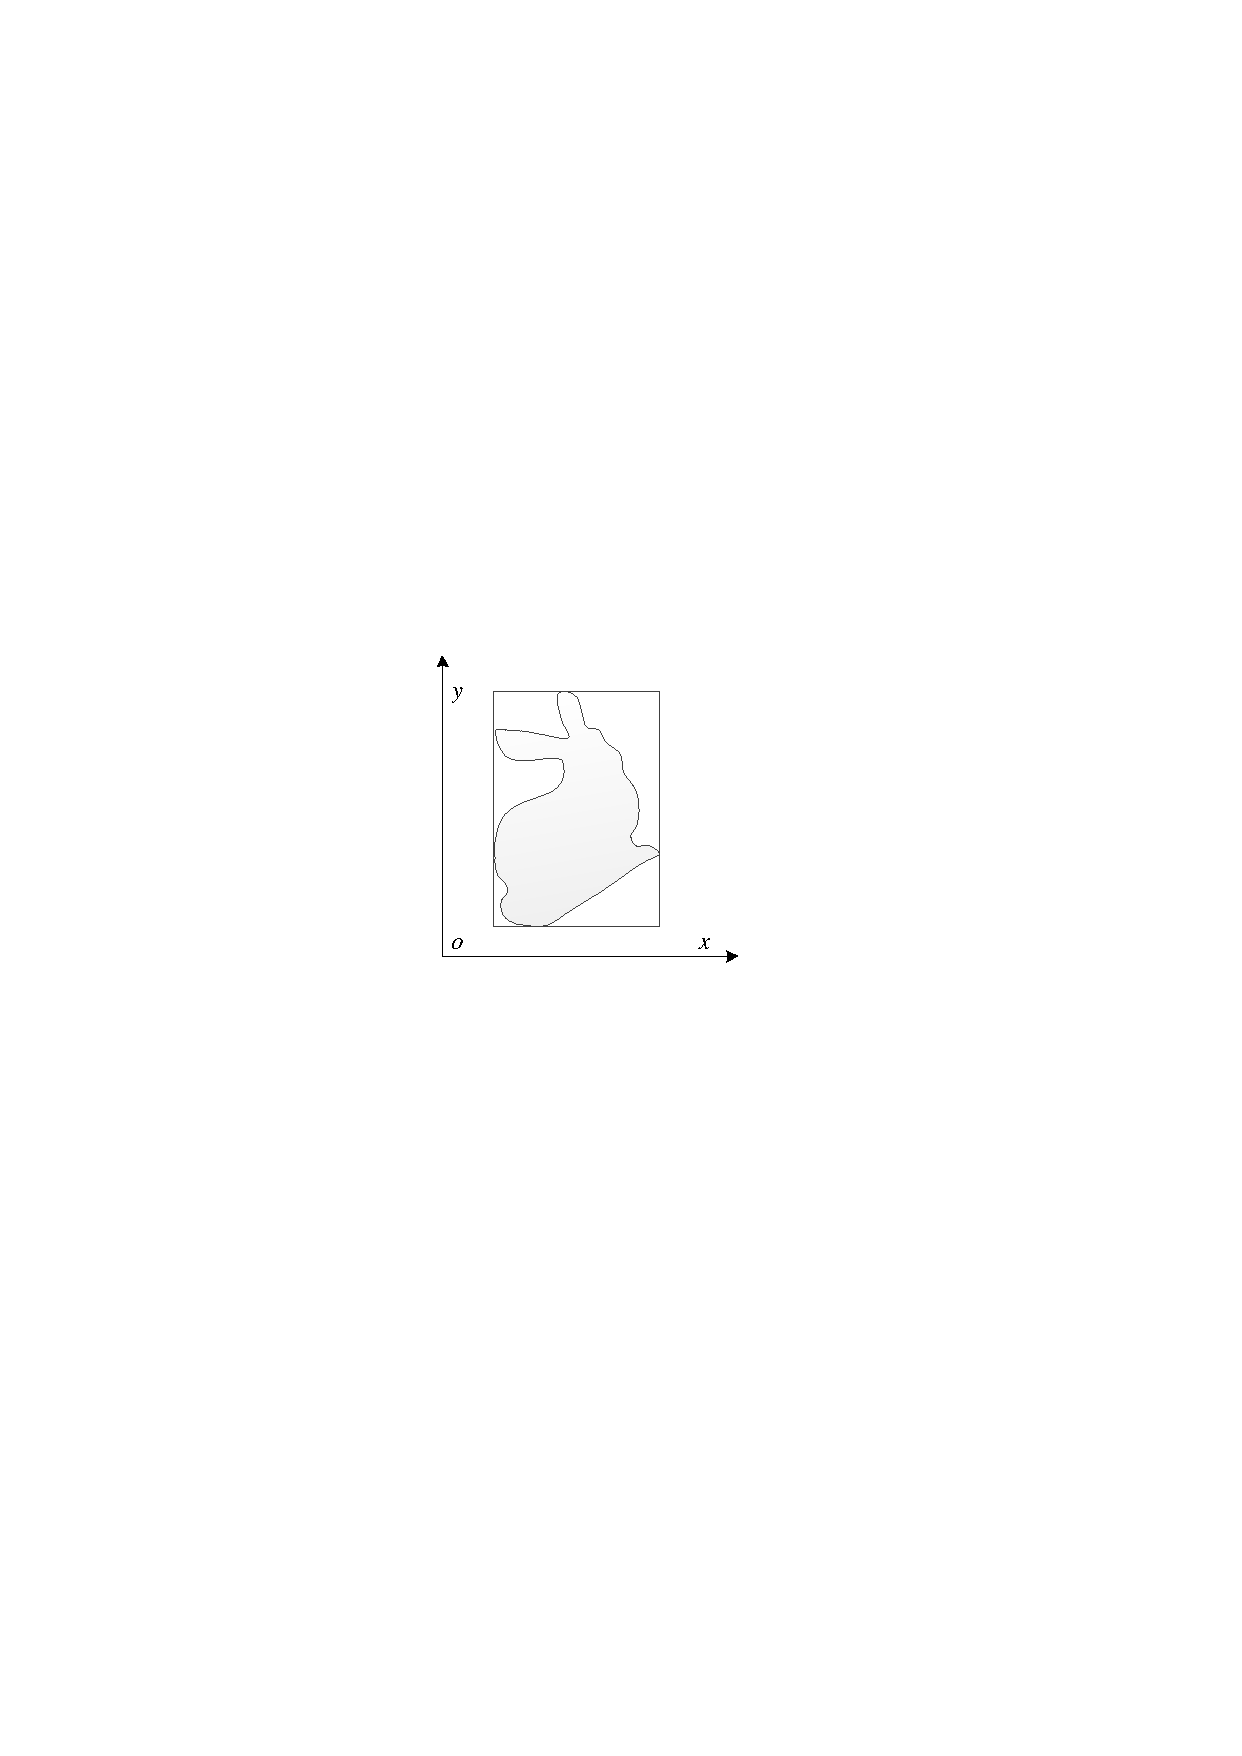
\includegraphics[width=1.5in]{bunny-2d-AABB.pdf}
  \caption{AABB 包围体}
  \label{fig:aabb-bunny}
\end{figure}

AABB~包围体的数据结构通常有3种方式:
\begin{inparaenum}[(1)]
\item 存储~AABB~包围体对角线上的两个极点,$Point_{min}$和$Point_{max}$,著名的计算几何库~CGAL\footnote{CGAL, Computational Geometry Algorithms Library, http://www.cgal.org}以此种方式存储;
\item 存储~AABB~包围体的中心点和各个方向的半径,$Point_{center}$和$Vector_{radius}$,如~SOLID\cite{bergen1997efficient};
\item 存储~AABB~包围体的极小点和各个方向的延伸长度\cite{ericson2005real},$Point_{min}$和$Vector_{extent}$。
\end{inparaenum} 

一方面~AABB~包围体之间的相交测试较简单,以数据结构为存储两个极点为例,只需要比较各个坐标值之间的大小即可。
但另一方面,通常情况下与原始模型的近似性较差,因其包围体的边沿着坐标轴方向可能会留较多的空白空间。

\subsection{OBB 包围体}

~OBB(Oriented Bounding Box)包围体是带方向的包围盒,可看作是~AABB~包围体沿任意方向转动一定角度后构成的包围体,因此通常情况下,~OBB~较~AABB~而言可以更紧致地贴近原始模型。
如图\ref{fig:obb-bunny}所示为平面图形~Bunny~的~OBB~包围体。

\begin{figure}[H] % use float package if you want it here
  \centering
  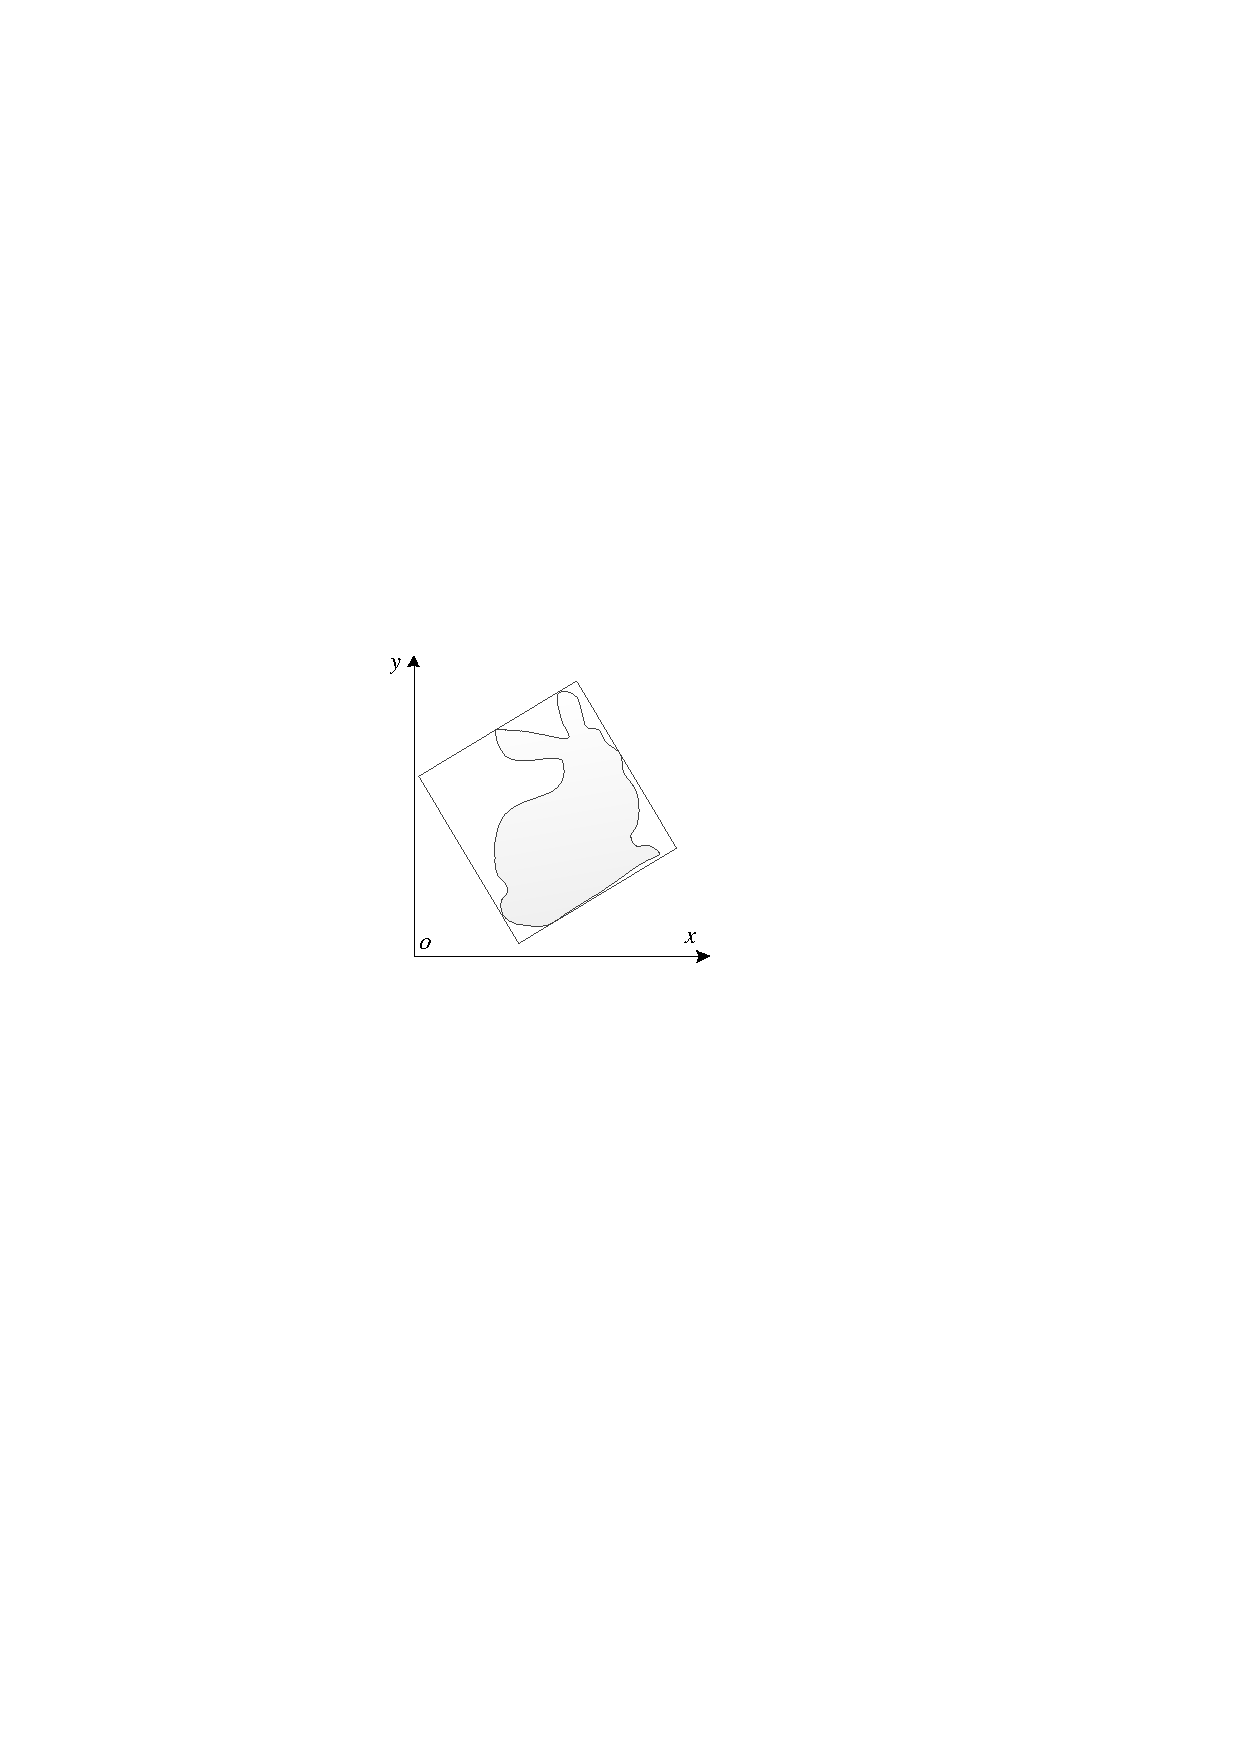
\includegraphics[width=1.5in]{bunny-2d-OBB.pdf}
  \caption{OBB 包围体}
  \label{fig:obb-bunny}
\end{figure}

与~AABB~类似,OBB~包围体的数据存储方式也可以有多种,最常用的是存储中心点,局部坐标架以及各个方向上的半径\cite{gottschalk1996obbtree}。因为~OBB~包围体的方向是任意的,有不少学者研究如何得到更加紧致的~OBB。

最早可追溯到由~O'Rourke~\cite{o1985finding}提出的$O(n^3)$
算法,文献\onlinecite{barequet2001efficiently}中提出了一种方法理论上可以在$O(n
+ 1/ \epsilon ^{4.5} )$复杂度内计算出一个近似最小~OBB($\epsilon$
为近似误差,即得到的$V\leq(1+\epsilon)\times V_{min}$,
其中$V$表示~OBB~的体积,$V_{min}$为最小~OBB~的体积),实际应用中通常实现的算法复杂度为$O(nlogn + n/
\epsilon ^{3} )$。~C.K.Chan~ \cite{chan2001determination}
提出了另外一种迭代的算法可以计算出误差范围内最小的~OBB~包围体,该算法适用于点数量较多(超过1万个点)的模型。

与~AABB~相比,~OBB~之间的相交测试稍复杂,需将二者转换到同一坐标系下进行计算,但其能更好的逼近原始模型。

\subsection{Sphere 包围体}

球形(Sphere)包围体,也称包围球(二维情况下即为包围圆,下同),即用一个半径尽量小的球包住给定所有点,该问题的求解是计算几何中的经典问题最小包围球的变种。
如图\ref{fig:sphere-bunny}所示为平面图形~Bunny~的~Sphere~包围体。

\begin{figure}[H] % use float package if you want it here
  \centering
  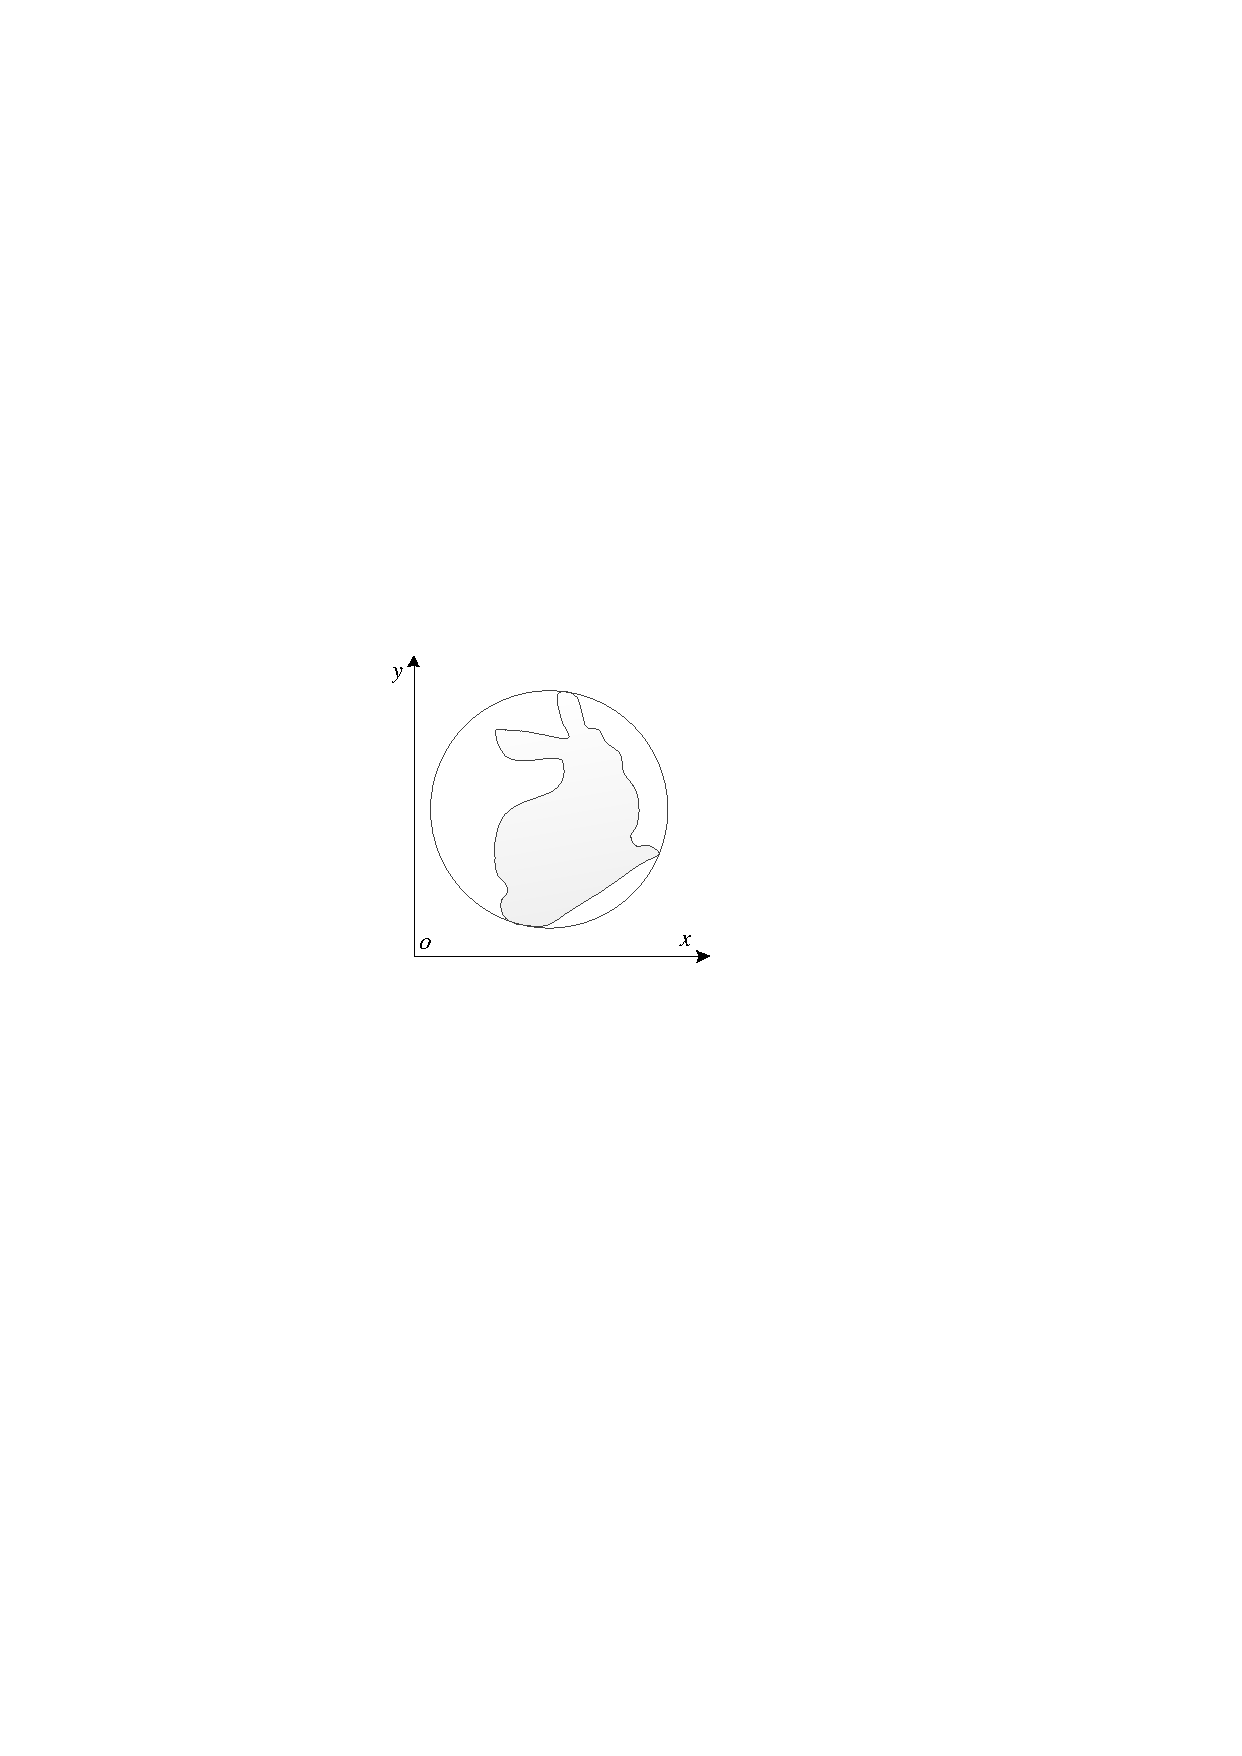
\includegraphics[width=1.5in]{bunny-2d-Sphere.pdf}
  \caption{Sphere 包围体}
  \label{fig:sphere-bunny}
\end{figure}

包围球的数据结构较简单,只需要球心和半径。一种最简单的计算一个包围求的方法是将相应~AABB~包围体的中心点作为球心,半径是为~AABB~各方向半径的最大值,这种方法虽然计算较快,但得到的包围体往往不够紧致。为了得到最小包围球,~E.Welzl~\cite{Welzl1991Smallest}
提出了一种线性的随机算法求出最小包围球。~T.Larsson~\cite{larsson2008fast}提出了一种快速简单的算法,该算法基于选择$k$个极点生成$k/2$个方向构造包围球,因而称为~EPOS~(Extremal Points Optimal Sphere~)算法,可以自定义$k$ 的值,能够给执行时间和包围盒紧致性之间进行调整折衷,提高了灵活性。

测试两个包围球是否相交较简单,只需判断两个球心之间的距离是否大于两个球半径之和即可。

\subsection{$k$-DOP 包围体}

$k$-DOP(Discrete Orientation Polytope)包围体是一个由$k$个固定方向的半平面相交构成的凸多面体,其最早思想来源于~TL.Kay~\cite{Kay1986Ray}
等人提出的用于解决光线追踪的问题,~$k$-DOP~术语是由~J.Klosowski~等人\cite{klosowski1998efficient}
在1998 年用于解决碰撞检测问题时提出的,有学者也称~$k$-DOP~为$k$-FDH($k$-Fixed
Directions Hull)\cite{weiyingmei2001}。
在二维(三维)平面上,~k-DOP~就是一个由$k/2$对平行的固定方向的边(面)围成的凸多边形(多面体),其中$k\in\mathbb{N}$,$k\geq4$($k\geq6$)。如图\ref{fig:8dop-bunny}所示,为平面图形~Bunny~的$8$-DOP。

\begin{figure}[H] % use float package if you want it here
  \centering
  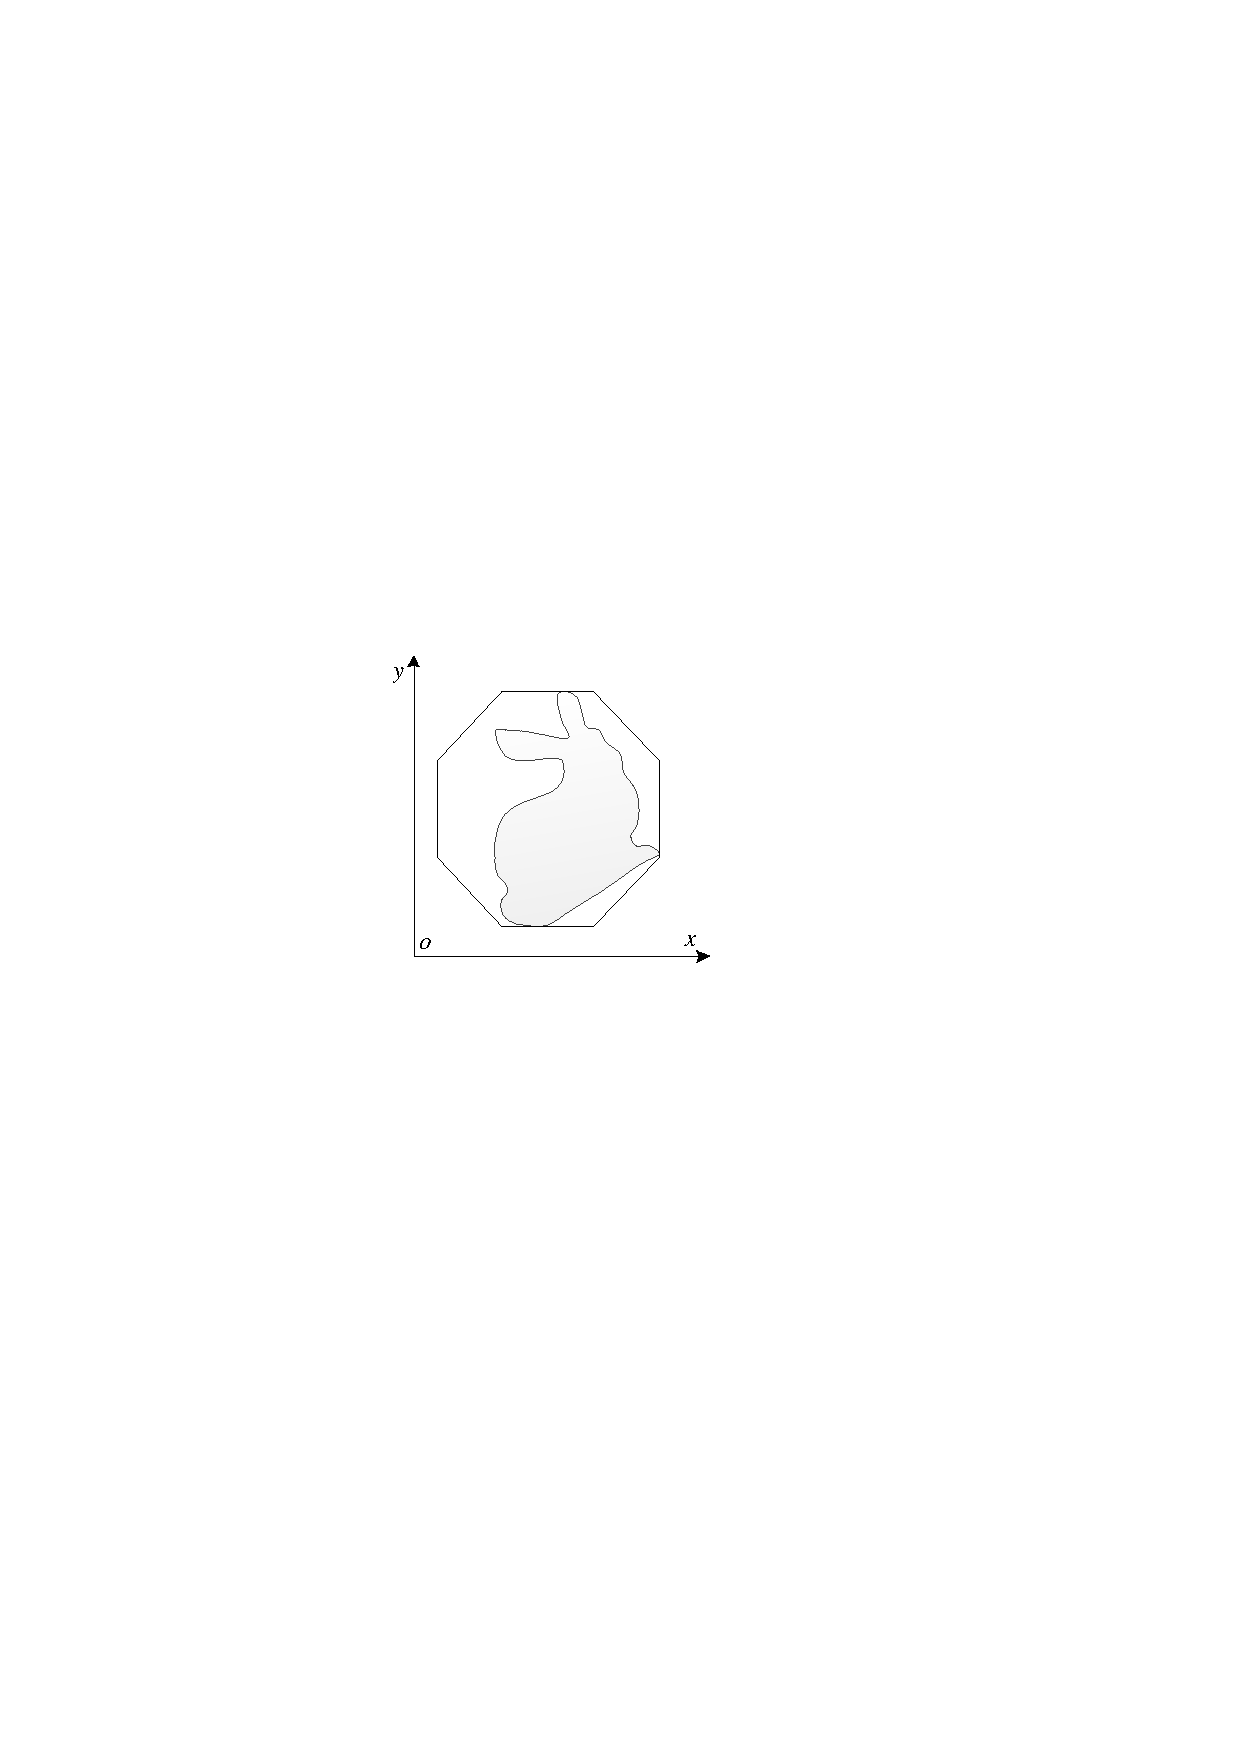
\includegraphics[width=1.5in]{bunny-2d-8DOP.pdf}
  \caption{$k$-DOP 包围体($k=8$)}
  \label{fig:8dop-bunny}
\end{figure}

对于$k$-DOP~中的每一个方向,可以由相应边(面)的法向决定,其数据结构一般用$k/2$个半平面的法向,再加上模型在各个方向上的投影的极值即可。因为$k$-DOP~的方向固定,$k$值确定后,相应的法向也随即确定,所以只需要存储各个方向的极值即可。当$k$-DOP~用于碰撞检测或可视化时,一般还需存储包围体的各个顶点。

与其他几种包围盒相比较而言,$k$-DOP~是取包围体存储计算和相交测试耗费时间的一个折衷,且可以通过修改$k$的值来提高包围体的灵活性。

\subsection{Convex hull 包围体}

凸包(Convex hull)是在计算几何中出现的概念,被定义为包含点集模型的最小凸集\cite{dengcg},
因此~Convex hull~包围体是最紧致的凸包围体,能够更好地近似模型本身。
包围体的紧致程度以凸包为衡量标准,一个包围体的紧致性 $\tau$ 按照如下公式计算:

\begin{equation}
\tau = \frac{V(CH)}{V(BV)}
\end{equation}
其中,$V(CH)$为凸包的体积,$V(BV)$~为包围体的体积,按照此公式计算出来的$\tau$越接近1表明其越紧致,凸包最紧致,其紧致性值1。

图\ref{fig:convexhull-bunny}为二维凸包的示例。

\begin{figure}[H] % use float package if you want it here
  \centering
  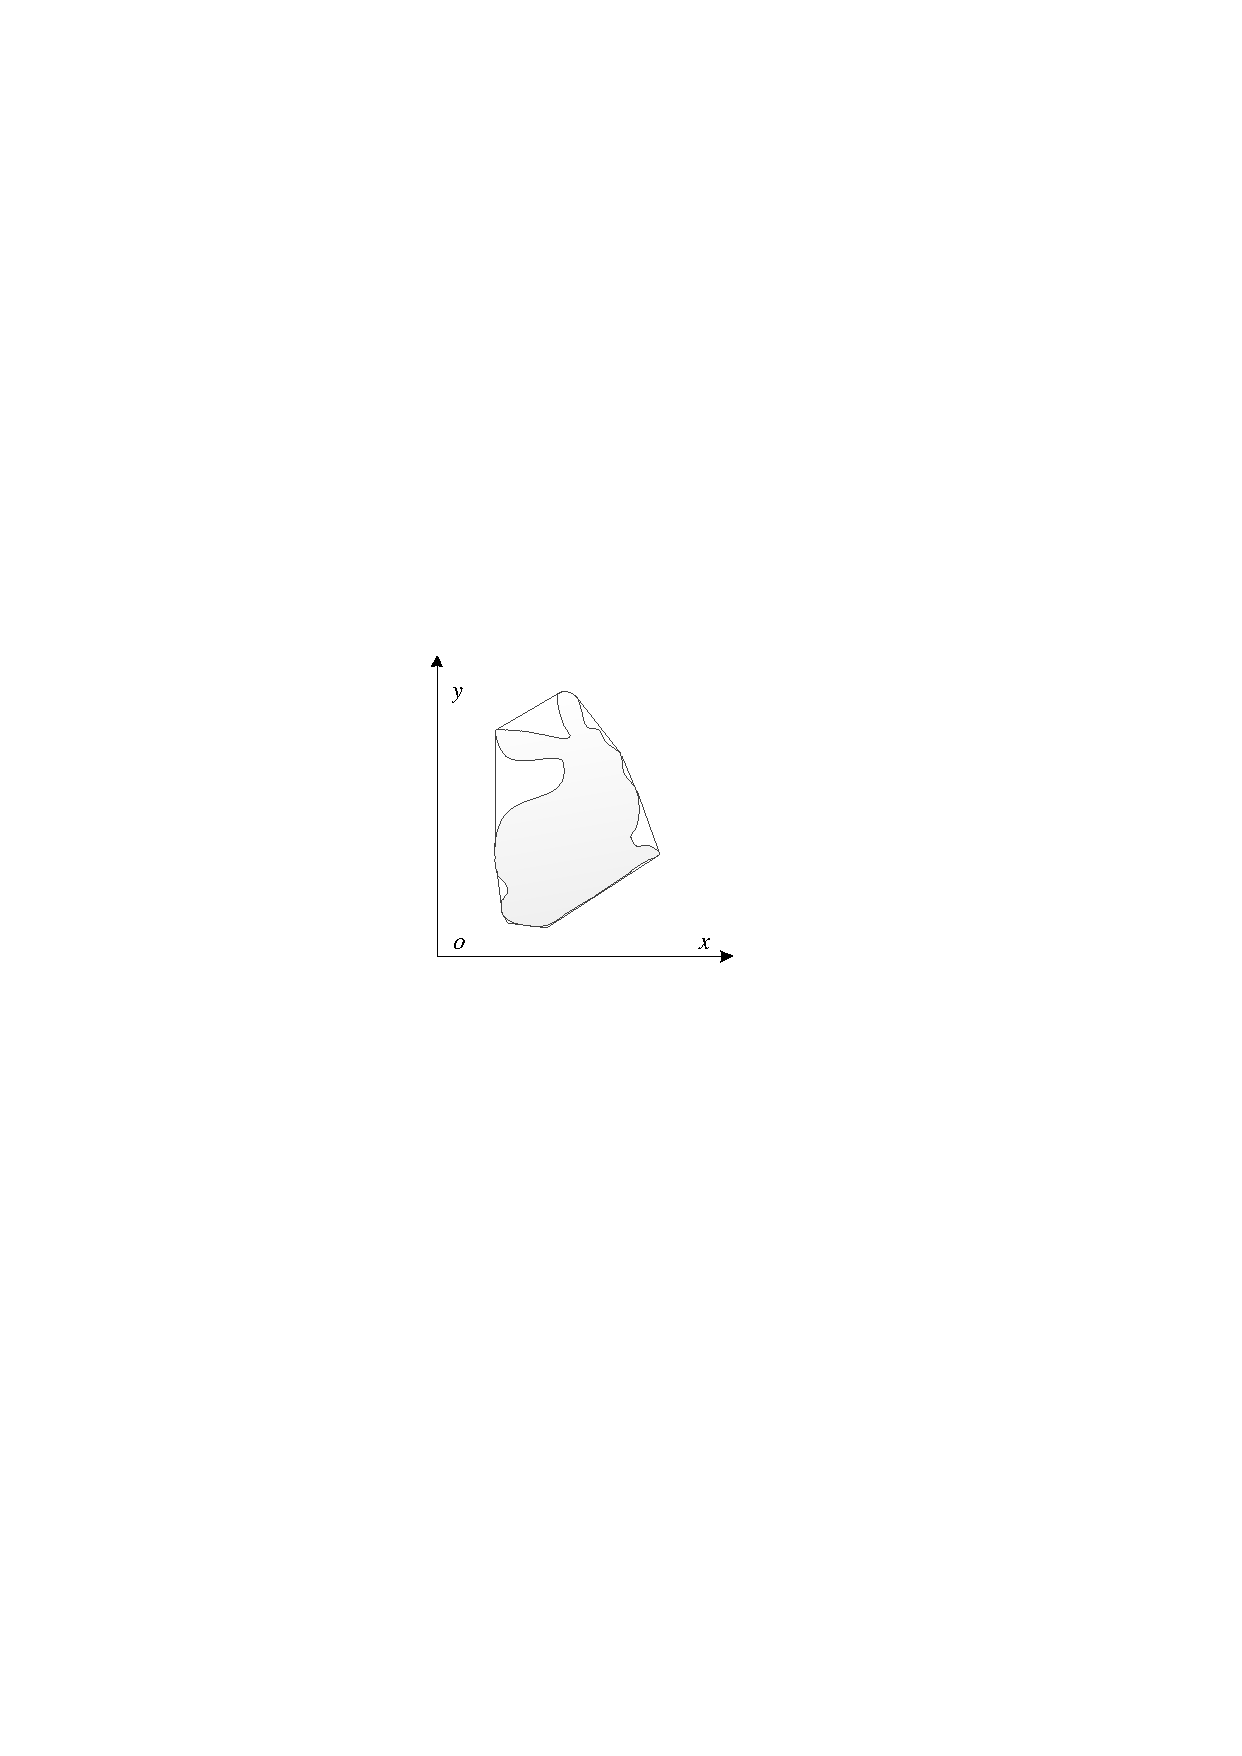
\includegraphics[width=1.5in]{bunny-2d-Convexhull.pdf}
  \caption{Convex hull 包围体}
  \label{fig:convexhull-bunny}
\end{figure}

常用的凸包构造算法有~Gift wrapping~\cite{Chand1970An},复杂度最坏情况下为$O(n^2)$,构造凸包的算法时间复杂度下限为$O(n\log n)$,如~Preparata~提出的分治算法\cite{Preparata1977}。
当模型点集较大时,包围体涉及到的面片数量太多,做相交测试等相关计算时耗费时间较久,同时也耗费较多存储空间。因此~Convex hull~包围体不太适用于大模型。
为此有学者在一些应用中用到近似凸包,
近似凸包可分为三类:近似外凸包、近似内凸包和近似凸包\cite{hossain2013constructing},近似内凸包完全在精确凸包内部,近似外凸包完全包含精确凸包,近似凸包即与精确凸包有相交的地方。
文献\onlinecite{bentley1982approximation,kavan2006fast}介绍了两种计算近似内凸包的算法,文
献\onlinecite{Zunie1992}介绍了一种计算二维近似外凸包算法,本文算法在生成法向时就借鉴了文献\onlinecite{bentley1982approximation}中的近似凸包算法。

\subsection{其他包围体}

除了以上几种常见的凸包围体外,不同学者在特定领域里也研究出以下另外几种包围体:\\
\begin{inparaenum}[(1)]
\indent
\item \textbf{Tribox} 可以看作是$k$-DOP~的一种特例,其中,二维中$k=8$ ,三维中$k=18$。 文献\onlinecite{crosnier1999tribox} 中提出的方法可以方便构造~Tribox~层次结构,并应用于模型分解中,当投影方向固定时,对于运动对象,更新其~Tribox~包围体也比较方便。 \\ 
\indent
\item \textbf{Swept-sphere}
是由~Eric.Larsen~等人\cite{Larsen1999Fast}提出的一种用于查询两个物体之间准确和近似相隔距离的解决方案,因而也用于碰撞检测的应用当中,该包围体有多种变种。原文中给出了球沿直线做拉伸构成的~Line-swept-sphere(如图\ref{fig:subfig-bv-swept-sphere}所示)
以及沿矩形拉伸构成的~Rectangle-swept-sphere~等阐述,并提出了构造层次结构包围体的算法,还对哪些包围体合适做碰撞检测,哪些包围体合适做最近距离计算做了分析和说明,更多内容可以参考文献\onlinecite{Larsen1999Fast}。\\
\indent
\item \textbf{Sphere-shell}
文献\onlinecite{krishnan1997spherical}给出了一种“球壳”(Sphere-shell)包围体,该包围体由两个同球心不同半径的球中间围成的壳与锥点为球心的锥面相交部分构成,如图\ref{fig:subfig-spherical-shell}所示。这种球壳包围体有利于非结构化的模型、多边形集合(Polygon
soups~)模型之间(如简单多边形,样条曲面构成的模型)的相隔距离计算或者进行碰撞检测。\\
\indent
\item \textbf{Zonotopes} 2003 年,~Leonidas
J.Guibas~\cite{Guibas2003Zonotopes}等人利用对偶的方法提出了一种用线段表示三维包围盒的隐式表达法,称其为~Zonotopes(二维称为~Zonogon),这种方法不用显示描述记录构成包围盒的多面体的每个面,节省存储,而同样能够在较快的时间内进行碰撞检测等。\\
\indent
\item \textbf{其他}
还有如图\ref{fig:subfig-bv-cylinder}所示的圆柱形\cite{Schomer2000Smallest}、图\ref{fig:subfig-bvcone}所示的圆锥形\cite{held1997erit}和如图\ref{fig:subfig-bv-ellipse}所示的椭球形\cite{Wang2004Efficient}等等包围体。
\end{inparaenum}

\begin{figure}[H]
  \centering%
  \subcaptionbox{圆柱形包围体\label{fig:subfig-bv-cylinder}}%[3cm] %标题的长度
    {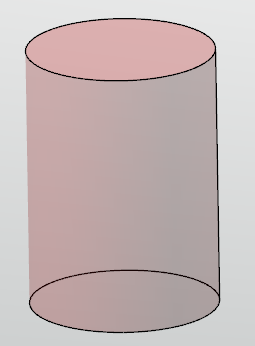
\includegraphics[height=4cm]{bv-cylinder.png}}
  \subcaptionbox{Sphere-shell~包围体\label{fig:subfig-spherical-shell}}
    {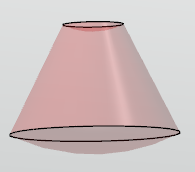
\includegraphics[height=4cm]{bv-spherical-shell.png}}
  \subcaptionbox{圆锥形包围体\label{fig:subfig-bvcone}}
    {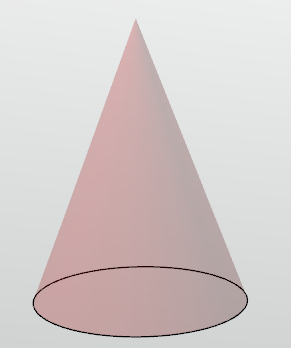
\includegraphics[height=4cm]{bv-cone.png}}
  \\
  \subcaptionbox{椭球形包围体\label{fig:subfig-bv-ellipse}}
    {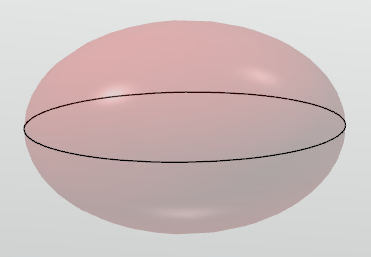
\includegraphics[height=4cm]{bv-ellipse.png}}
  \subcaptionbox{Swept-sphere~包围体\label{fig:subfig-bv-swept-sphere}}
    {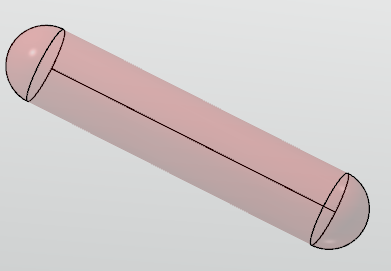
\includegraphics[height=4cm]{bv-swept-sphere.png}}
  \caption{其他包围体}
  \label{fig:bv-others}
\end{figure}

\subsection{包围体的应用}

包围体常见的应用领域有真实感渲染如可见面判别、视域剔除\cite{assarsson2000optimized},光线追踪\cite{wald2007ray}等。
在光线追踪算法中,包围体用于检测光线是否与物体相交,如果光线没有与包围体相交,则肯定不会与包围体内的物体模型相交,进而就不用渲染显示该物体。
另外更常见的应用就是碰撞检测\cite{wangzhiqiang1999},大多数碰撞检测算法都用到了各式各样的包围体以加速,如
\onlinecite{larsson2006dynamic,madera2009hybrid,vogiannou2010enhancing,chang2010efficient,tang2010fast,zhigang2010efficient} 等。

有不少文献将包围体和模型简化技术结合起来,例如~Kai Huebner~等人\cite{huebner2008minimum}在利用文献
\onlinecite{barequet2001efficiently}中提出的构造最小~OBB~包围体算法的基础上将物体分解成多个~OBB~包围体,用这些~OBB~包围体近似原始模型用于机器人抓取中,如图\ref{lbl:Huebner2008-example}所示。
类似的还有~Sphere~包围体的分解\cite{hubbard1996approximating}(如图\ref{lbl:hubbard1996approximating-example}),~Tribox~的分解\cite{crosnier1999tribox}等。

\begin{figure}[H]
  \centering
  \subcaptionbox{模型简化成~OBB~包围体\cite{huebner2008minimum}\label{lbl:Huebner2008-example}}%[3cm] %标题的长度
    {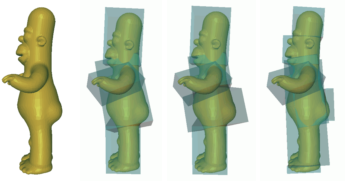
\includegraphics[height=4cm]{Huebner2008-example.png}}
  \subcaptionbox{模型简化成~Sphere~包围体\cite{hubbard1996approximating}\label{lbl:hubbard1996approximating-example}}
    {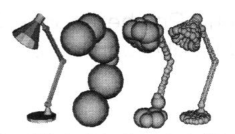
\includegraphics[height=4cm]{hubbard1996approximating-example.png}}
  \caption{包围体应用于模型简化}
  \label{lbl:bounding-voluems-used-in-shape-approximation}
\end{figure}

Jyh-Ming Lien~\cite{lien2006approximate2d}等人在06年提出一种方法可以将给定的多边形(包括含有孔洞的)分解成多个凸多边形,并提供不同种精度的分解,可以应用于~LoD(Level of
Detail,多层次细节)~,并在07年将其扩展到三维\cite{lien2007approximate3d},即提出了一种方法将原始实体模型近似为层次结构的凸包围多面体,如图\ref{lbl:lien2007approximate-example}
所示,对图中的原始模型进行准确凸分解(~ECD,Exact Convex
Decompositions~)将得到726240个组成部分,而近似凸分解(~ACD,Approximate Convex
Decompositions~)仅得到98个组成部分,同时保持了原始模型的大致形状,这大大加速了渲染过程。

\begin{figure}[H]
\centering
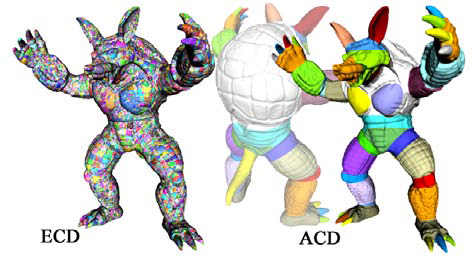
\includegraphics[width=3in]{lien2007approximate-example.png}
\caption{层次结构凸包围多面体的精确构造和近似构造\cite{lien2007approximate3d}}
\label{lbl:lien2007approximate-example}
\end{figure}
这种分解还可以应用于多种应用,例如运动规划(~Motion planning~),网格生成(~Mesh generation~),点定位(~Point location~)问题等等,更多内容可以参考\cite{lien2008approximate} 以及~Jyh-Ming Lien~ 的博士学位论文\cite{lien2006approximatephd}。

文献\cite{attene2008hierarchical}利用一种类似的方法将原始3D模型分解成一个具有层次结构的模型(图\ref{lbl:attene2008hierarchical-example:subfig1}所示),最顶层将是整个模型的凸包。将该算法应用到3D编辑环境中,能够更加方便地让用户选择模型的某个部分进行交互设计。效果如图\ref{lbl:attene2008hierarchical-example:subfig2} 所示,用户选择模型的头部,并进行拖拽能够较快速得到模型新的外观。\footnote{详情可参考视频:http://www.readcube.com/articles/10.1111/j.1467-8659.2008.01271.x }

\begin{figure}[H]
  \centering
  \subcaptionbox{层次结构的分解\label{lbl:attene2008hierarchical-example:subfig1}}
    {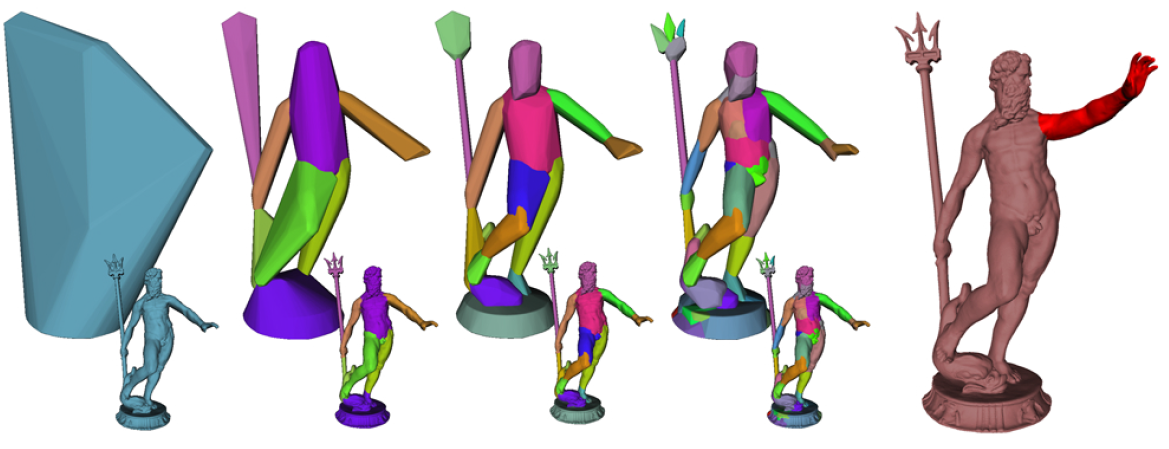
\includegraphics[height=2.8cm]{attene2008hierarchical-example-0.png}}
  \subcaptionbox{区域选择进行交互设计 \label{lbl:attene2008hierarchical-example:subfig2}}
    {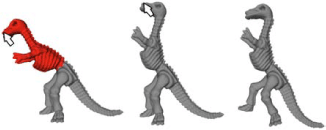
\includegraphics[height=2.8cm]{attene2008hierarchical-example.png}}
  \caption{层次结构的凸包围体及其应用于交互设计\cite{attene2008hierarchical}}
  \label{lbl:attene2008hierarchical-example}
\end{figure}

随着计算机软件技术和硬件的发展,有不少并行算法来计算包围体。
文献\cite{karlsson2010parallel}利用~Intel~单指令多数据流(Single Instruction
Multiple Data~,简称SIMD)~SSE~指令集和~OpenMP~实现了对~AABB~,~OBB~和~$k$-DOP~的计算。
文献\cite{lauterbach2009fast}提出了在~统一计算设备架构(Compute Unified Device
Architecture,简称CUDA,后同)~平台上基于~GPU~构造~AABB~包围体树的方法并应用于光线追踪。

\section{碰撞检测算法}
\label{sec:collisiondetection}

碰撞检测是许多应用的基础,例如在~3D~游戏,物理仿真,机器人,虚拟现实等。本节将就碰撞检测问题的分类和基于包围体树的算法进行阐述。

\subsection{碰撞检测算法的分类}
\label{sec:cd-category}

碰撞检测算法按照不同的分类标准可以有不同的分类方法。
根据其利用的加速结构不同大致可以分为两类,
一类是空间划分树(Spatial Partition Tree~,四叉树,八叉树,~KD~
树等),如文献\onlinecite{Melax2000}就提出了一种基于~BSP~的算法应用于~3D~游戏中的碰撞检测。
另外一种就是层次结构包围体(Bounding Volume Hierarchies
,简称~BVH,也称包围体树),如在\ref{sec:convex-bv}提到的~AABB~,~OBB~等包围体树。
包围体树跟常见的空间划分树最大的区别就是,在~BVH~中的两个或多个包围体可以包含相同的空间,而空间划分树的每个划分结构是分离的,且在~BVH~中,父节点不一定必须完整包含子节点,只需要包含子节点对应原始物体的那部分即可\cite{ericson2005real}。 
根据参与碰撞检测的物体模型的表现形式,又可以分为凸体模型或凹体模型,多边形或者三角网格模型,CSG~(Constructive
Solid Geometry,构造实体几何)模型,隐式方程或者参数表达曲面模型等,例如文献\onlinecite{Zeiller1995}就讨论了计算机动画系统中基于CSG模型的碰撞检测算法,GJK~算法\cite{Science1999}就是针对凸体模型之间的碰撞检测算法。
根据碰撞检测的模拟环境划分,又可以分为成对(Pair
Processing)碰撞检测和多体(Nbody
Processing)碰撞检测,刚体和柔性模型的碰撞检测以及静态和动态(连续)碰撞检测\cite{lin1998collision}。
文献\onlinecite{jimenez20013d}从碰撞检测的解决策略上做了系统的分类和总结,文中提到目前的碰撞检测都是从几何或代数的方法进行求解,其中几何方法主要利用投影、采样或者二者的结合的技术进行处理。

随着~3D~扫描仪的出现,近年来也出现了一些基于点云的碰撞检测算法。Klein Jan~等人\cite{klein2004point}首次在~EuroGraphics 04~上提出了点云的碰撞检测概念,同样利用了层次结构包围体进行加速检测,并提出了一个给定容差的判断点云模型之间是否相交的算法。
文献\cite{figueiredo2010efficient}将~AABB~包围体和~R~树结合起来,并从~OAABB(Overlapped AABB)中找出是否含有一个模型的点在容差范围内逼近另外一个点云模型以此判断是否发生相交。

随着计算机图形卡的产生,又不断涌现出基于~GPU~的碰撞检测并行算法,如文献\onlinecite{Zhang2007Interactive,hebing2009}等,利用~GPU~多线程技术提高碰撞检测的效率。

\subsection{基于包围体树的碰撞检测算法}
\label{sec:cd-bvh}

在第\ref{sec:convex-bv}节中介绍了在对原始几何模型进行求交判断之前先用其包围体判断是否相交有助于提高求交过程的性能,
通过将包围体组织成树形结构即层次结构包围体(BVH)能够将包围体预判阶段从理论上降低到对数时间复杂度(要求树是平衡的)。
当构造原始复杂模型的包围体树时,复杂模型会被拆分成多个部分,每个部分用某种包围体近似,这构成了树型结构的叶子节点,这些节点会按照某种分组策略进行合并成更大的包围体分别构成其父节点,如此递归,最终形成一颗树,树最顶端是一个包含住原始物体的最粗糙的包围体,如图\ref{lbl:bvh-example}
所示,为一个8层~AABB~包围体的~BVH(也可以看作是8层6-DOP的~BVH)。
\begin{figure}[H]
  \centering
  \subcaptionbox*{\label{lbl:bvh-bunny-center-0.png}}
    {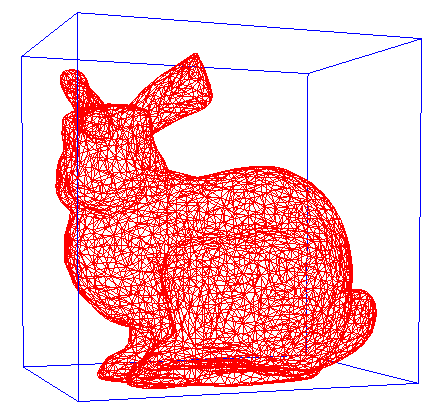
\includegraphics[height=2.8cm]{bvh-bunny-center-0.png}}
  \subcaptionbox*{\label{lbl:bvh-bunny-center-1.png}}
    {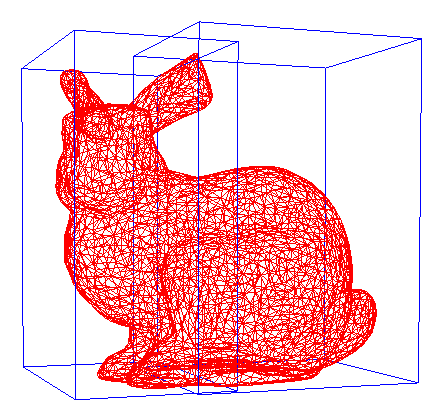
\includegraphics[height=2.8cm]{bvh-bunny-center-1.png}}
  \subcaptionbox*{\label{lbl:bvh-bunny-center-2.png}}
    {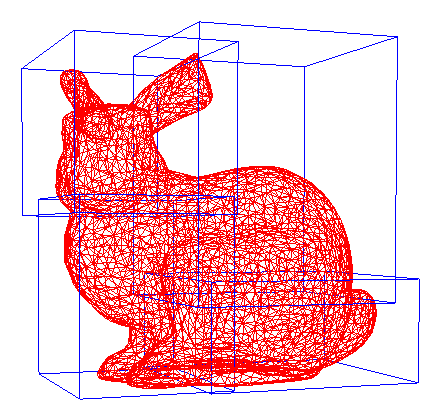
\includegraphics[height=2.8cm]{bvh-bunny-center-2.png}}
  \subcaptionbox*{\label{lbl:bvh-bunny-center-3.png}}
    {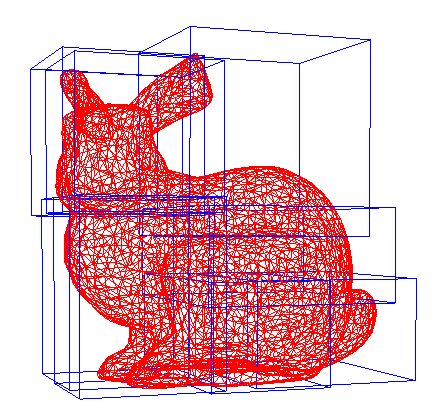
\includegraphics[height=2.8cm]{bvh-bunny-center-3.png}}
    \vspace{-0.3cm}
  \\\hspace{0.5cm} 
  \subcaptionbox*{\label{lbl:bvh-bunny-center-4.png}}
    {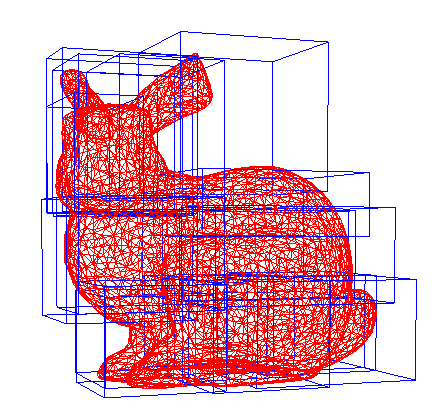
\includegraphics[height=3.0cm]{bvh-bunny-center-4.png}}
  \subcaptionbox*{\label{lbl:bvh-bunny-center-5.png}}
    {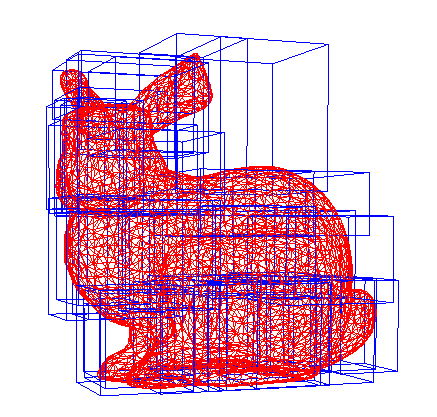
\includegraphics[height=3.0cm]{bvh-bunny-center-5.png}}
  \subcaptionbox*{\label{lbl:bvh-bunny-center-6.png}}
    {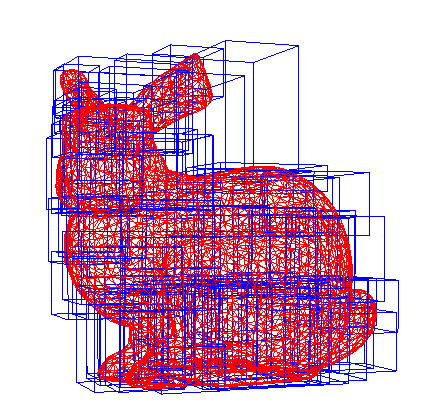
\includegraphics[height=3.0cm]{bvh-bunny-center-6.png}}
  \subcaptionbox*{\label{lbl:bvh-bunny-center-7.png}}
    {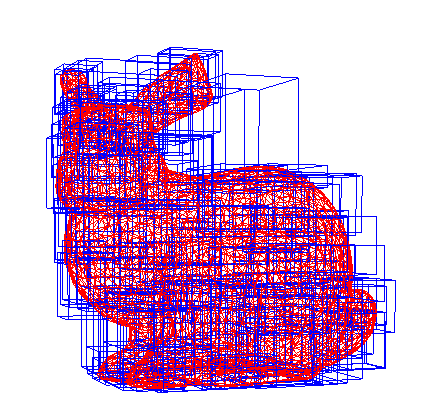
\includegraphics[height=3.0cm]{bvh-bunny-center-7.png}}
\caption{八层~BVH~示例}
\label{lbl:bvh-example}
\end{figure}

在碰撞检测算法中,一般会对模型进行预处理建立起各自的~BVH~树,当两个模型进行相交检测时,自顶向下遍历两棵~BVH~树,若父节点没有相交,则没有必要进行子节点的相交测试,自顶向下的遍历算法如算法~\ref{alg:traverse-bvh-tree}~所示。

\begin{algorithm}
\algsetup{linenosize=\tiny}
\small
\caption{$TraverseBVHTree(node_1, node_2)$}
\label{alg:traverse-bvh-tree}
\begin{algorithmic}[1]
\REQUIRE
$node_1$,$node_2$:BVH~树中的节点1、节点2
\ENSURE
是否相交
\IF{$node_1.bv \cap node_2.bv = \emptyset$} 
    \RETURN \FALSE \COMMENT{包围体重合测试, 包围体不相交直接返回}
\ELSE
    \IF {$node_1.children = \emptyset$}
         \IF {$node_2.children = \emptyset$}
            \RETURN {$CheckIntersection(node_1.primitives, node_2.primitives)$}
            \COMMENT{最底层叶子节点原生几何相交测试}
         \ELSE
            \FORALL {$child \in node_2.children$}
                \STATE $TraverseBVHTree(node_1, child)$ \COMMENT{递归调用}
            \ENDFOR
         \ENDIF
    \ELSE
         \FORALL {$child \in node_1.children$}
            \STATE $TraverseBVHTree(child, node_2)$  \COMMENT{递归调用}
         \ENDFOR
    \ENDIF
\ENDIF
\end{algorithmic}
\end{algorithm}

从算法~\ref{alg:traverse-bvh-tree}~可以看出,基于~BVH~的碰撞检测算法性能的好坏关键在于两个操作,一是分别来自两个~BVH~内部节点包围体之间的相交测试,二是~BVH~最底层叶子节点内的原生几何相交测试,常常利用~$T_{cost}
= n_v * C_v + n_p * C_p$ 来衡量单个相交测试的所付出的代价,其中$n_v$
和$n_p$分别表示参与包围体节点相交测试的数量和参与原始几何相交测试的数量,$C_v$和$C_p$则表示相应的平均测试耗费的代价\cite{klosowski1998efficient}。
当运动场景或连续碰撞的模型之间的碰撞检测时,往往还需要考虑到因物体模型旋转平移等变换产生的包围体的更新所付出的代价,即上述代价函数变成$T_{cost}
= n_v * C_v + n_p * C_p + n_u *
C_u$,要提高碰撞检测的性能,就得想办法减小$T_{cost}$的值。本文的算法主要关注于静态场景。

不同的包围体,上述代价函数各个值不同,对于不同的应用场景,可能需要选择不同的包围体进行加速碰撞检测。
文献\onlinecite{zhigang2010efficient}从包围体的构造难度,包围体的紧致性,包围体之间相交测试复杂性及包围体在运动过程中的更新代价几个方面对五种常见的包围体进行了比较,如表\ref{lbl:table:bv-comp}所示。
可以看出,各种包围体有各自的优缺点和适用场景,因此,很多研究人员充分利用各种包围体的优点,将多种包围体结合在一起组成新的组合包围体。
文献\cite{chang2010efficient}利用~OBB~包围体相对的紧致优点和球形包围体相交测试简单性的优点进行组合,构造~OBB-Sphere~包围体,在进行相交测试时,先利用球形包围体进行测试,如果相交再用~OBB~进行测试。
类似的,文献\cite{zhigang2010efficient}同时利用更加紧致的$k$-DOP~和~Sphere~包围体构造$k$-DOP-Sphere~包围体。

\begin{table}[H]
\centering
\caption{碰撞检测中常用凸包围体比较}
\begin{tabular*}{13cm}{ccccc}
\toprule[1.2pt]
凸包围体 & 构造代价 & 相交测试简单性 & 紧致性 & 更新代价\\
\midrule[1pt]
AABB   & 1 & 2 & 4 & 3\\
OBB    & 4 & 4 & 3 & 2\\
Sphere & 2 & 1 & 5 & 1\\
k-DOP  & 3 & 3 & 2 & 4\\
Convex hull & 5 & 5 & 1 & 5 \\
\bottomrule[1.2pt]
\end{tabular*}
\label{lbl:table:bv-comp}
\end{table}


\section{本文主要内容}
\label{sec:structure}
本文着重讨论如何快速地生成紧致性可控的凸包围体以及将此包围体应用于静态场景的碰撞检测。
第一章首先介绍了当前各种凸包围体的特征及应用。然后再介绍了碰撞检测问题的背景和本文研究的基于凸包围体的碰撞检测算法。

第二章提出了紧致性可控的凸包围体$k$-CBP($k$-Convex Bounding Polyhedron)~的生成算法,紧致性可控主要通过凸包围体的平面数量$k$来调节。
该算法法首先利用近似内凸包和~$k$-means~聚类算法生成构成凸包围多面体~$k$~个截面的法向,
然后根据输入点集沿各法向搜索切点构成截面,最后由这些截面通过对偶映射的方式求交构成凸包围多面体。
在搜索截面过程中,提出了两种并行策略以加速搜索过程。实验结果表明,与同类算法相比,该方法能够更快地构造给定点集更紧致的凸包围多面体。

第三章提出了基于本文提出的$k$-CBP~包围体的碰撞检测算法,在包围体之间的相交测试时分别用~AABB~树的方式和基于~GJK~算法的两种方式进行。
实验结果表明本文提出的凸包围体能够有效加速碰撞检测算法。

第四章是对本文的研究工作进行总结,以及未来可以改进的方向。

% 
%%% Local Variables: 
%%% mode: latex
%%% TeX-master: t
%%% End: 

\chapter{凸包围体生成算法}
\label{cha:kcbp-construction}
从第~\ref{sec:convex-bv}~节可以看出包围体的紧致程度直接影响相应算法的效率,对于不规则形体, 常见的包围体往往不够紧致,凸包紧致但往往包含过多的面片数而增加算法的复杂性。

本文提出一种构造凸包围多面体的方法,该方法首先利用近似内凸包和~$k$-means~聚类算法生成构成凸包围多面体~$k$~个截面的法向。
然后根据输入点集沿各法向搜索切点构成截面, 最后由这些截面通过对偶映射的方式求交构成凸包围多面体。搜索截面过程中,各个法向的搜索过程相互独立互不影响,因此可以方便地利用~GPU~进行加速。
本文提出的方法的主要优势是:
\begin{inparaenum}[(1)]
\item 对给定点集可构造紧致的包围体;
\item 利用~GPU~加速,能够快速构造包围体;
\item 通过参数~$k$~调节凸包围多面体的简单性和紧致性,可适用于不同的应用场景。
\end{inparaenum}

由~$k$~个截面构成的凸包围多面体称为凸包围~$k$~面体($k$-Convex Bounding Polyhedron,简称~$k$-CBP), 可通过~$k$~个半空间定义:
\begin{equation}
\label{equ:kcbp_definition}
\left\{
\begin{array}{l}
    k\mbox{-CBP} = \mathop  \bigcap \limits_{i = 1}^k \bm{H_i} \\
    \bm{H_i} = \left\{ {\left. {\bm{p} \in {\mathbb{R}^3}} \right| \bm{n_i} \cdot \bm{p} \le {w_i}} , w_i \in \mathbb{R} \right\},
\end{array}
\right.
\end{equation}
其中,$\bm{n_i}$~是半空间~$\bm{H_i}$~的法向,方向指向包围体外部,
$w_i$~是输入点集中沿~$\bm{n_i}$~方向投影的最大值。
如图~\ref{fig:bunny}~所示是~Bunny~模型的凸包围~34~面体(34-CBP)。

\begin{figure}[htbp] 
\centering
  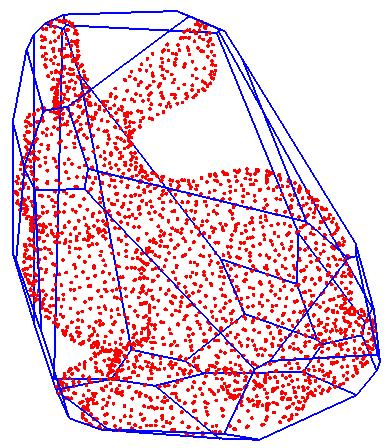
\includegraphics[width=1.5in]{bunny-34.png}
  \caption{~Bunny~模型的~34-CBP }
  \label{fig:bunny}
\end{figure}

本文算法的主要流程如图~\ref{lbl:kcbp-algorithm-flowchart}~所示,首先利用近似内凸包和~$k$-means~聚类算法生成构成凸包围多面体~$k$~个截面的法向,然后根据输入点集在~GPU~中沿各法向搜索切点构成截面,
最后由这些截面通过对偶映射的方式求交构成凸包围多面体。搜索截面需要多次扫描输入点集,在~CPU~中计算较耗时,因此用~GPU~加速使得算法整体性能得以提升,其他步骤在~CPU~计算即可。

\begin{figure}[htbp]
    \centering
    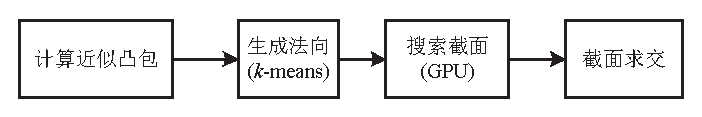
\includegraphics[width=5.5in]{kcbp-flowchart-x-aix.eps}
    \caption{构造~$k$-CBP~算法流程图}
    \label{lbl:kcbp-algorithm-flowchart}
\end{figure}

图~\ref{lbl:bunny-26-cbp-ch-ach}~从左至右分别显示了~Bunny~模型的~26-CBP、精确凸包和近似内凸包。
近似凸包是精确凸包的一种近似,与精确凸包外观相似但其构造复杂度降低,不少研究者利用该性质解决计算机图形学中很多问题\cite{hossain2013constructing}。

\begin{figure}[htbp] % use [htbp] to fix the position
\centering
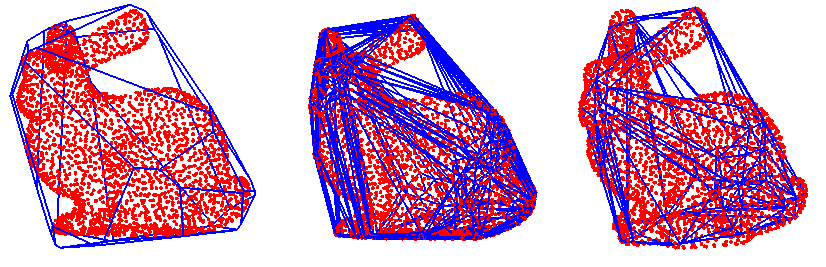
\includegraphics[width=5.0in]{26-bunny-ach-ch-kcbp.png}
\caption{~Bunny~模型的~26-CBP、凸包和近似内凸包}
\label{lbl:bunny-26-cbp-ch-ach}
\end{figure}

本文就利用了近似内凸包与精确凸包的相似性,从众多近似凸包面片的法向中通过~$k$-means~聚类算法生成构成凸包围多面体的~$k$~个法向。
本章后续部分将按步骤详细介绍算法的实现。
%由图可知, 近似内凸包的三角面片大致反映了精确凸包三角面片的分布情况,近似内凸包相应位置面积较大的三角面片对应到精确凸包的三角面片面积也较大, 因此该三角面片所在平面需尽量保留.

\section{截面法向的生成}
\label{sec:gen-normals}

截面法向的选定与多面体的紧致程度密切相关。
$k$-DOP\cite{klosowski1998efficient}~预先定义~$k/2$~对法向,且~$k$~值局限于6、14、18或26等少数几个,对于不同的模型其方向始终一致,导致其生成的多面体不能自适应模型,对于不规则形体的模型不够紧致。
与~$k$-DOP~相比,本文算法~$k$~值取值更灵活,因此可以根据不同需求不同应用场景更加灵活地选择需要的凸包围体。
根据经验,为了使凸包围多面体尽可能逼近凸包,在多面体数量一定的情况下需尽量保留凸包中面积较大的面。 
本文生成凸包围多面体的法向的流程是先通过一种线性算法\cite{bentley1982approximation}构造近似内凸包,然后从近似内凸包里选取面积最大的~$a$~个面的法向,最后用聚类算法从剩下的面中生成~$k-a$~个法向。
下面将介绍截面法向生成的主要步骤。

\subsection{近似内凸包生成聚类样本法向集}
\label{subsec:ach-gen-normals}

以平面点集的近似内凸包为例说明初始法向集的生成。

\begin{figure}[htbp]
  \centering
  \subcaptionbox{分组\label{lbl:subfig-split-groups}}{
    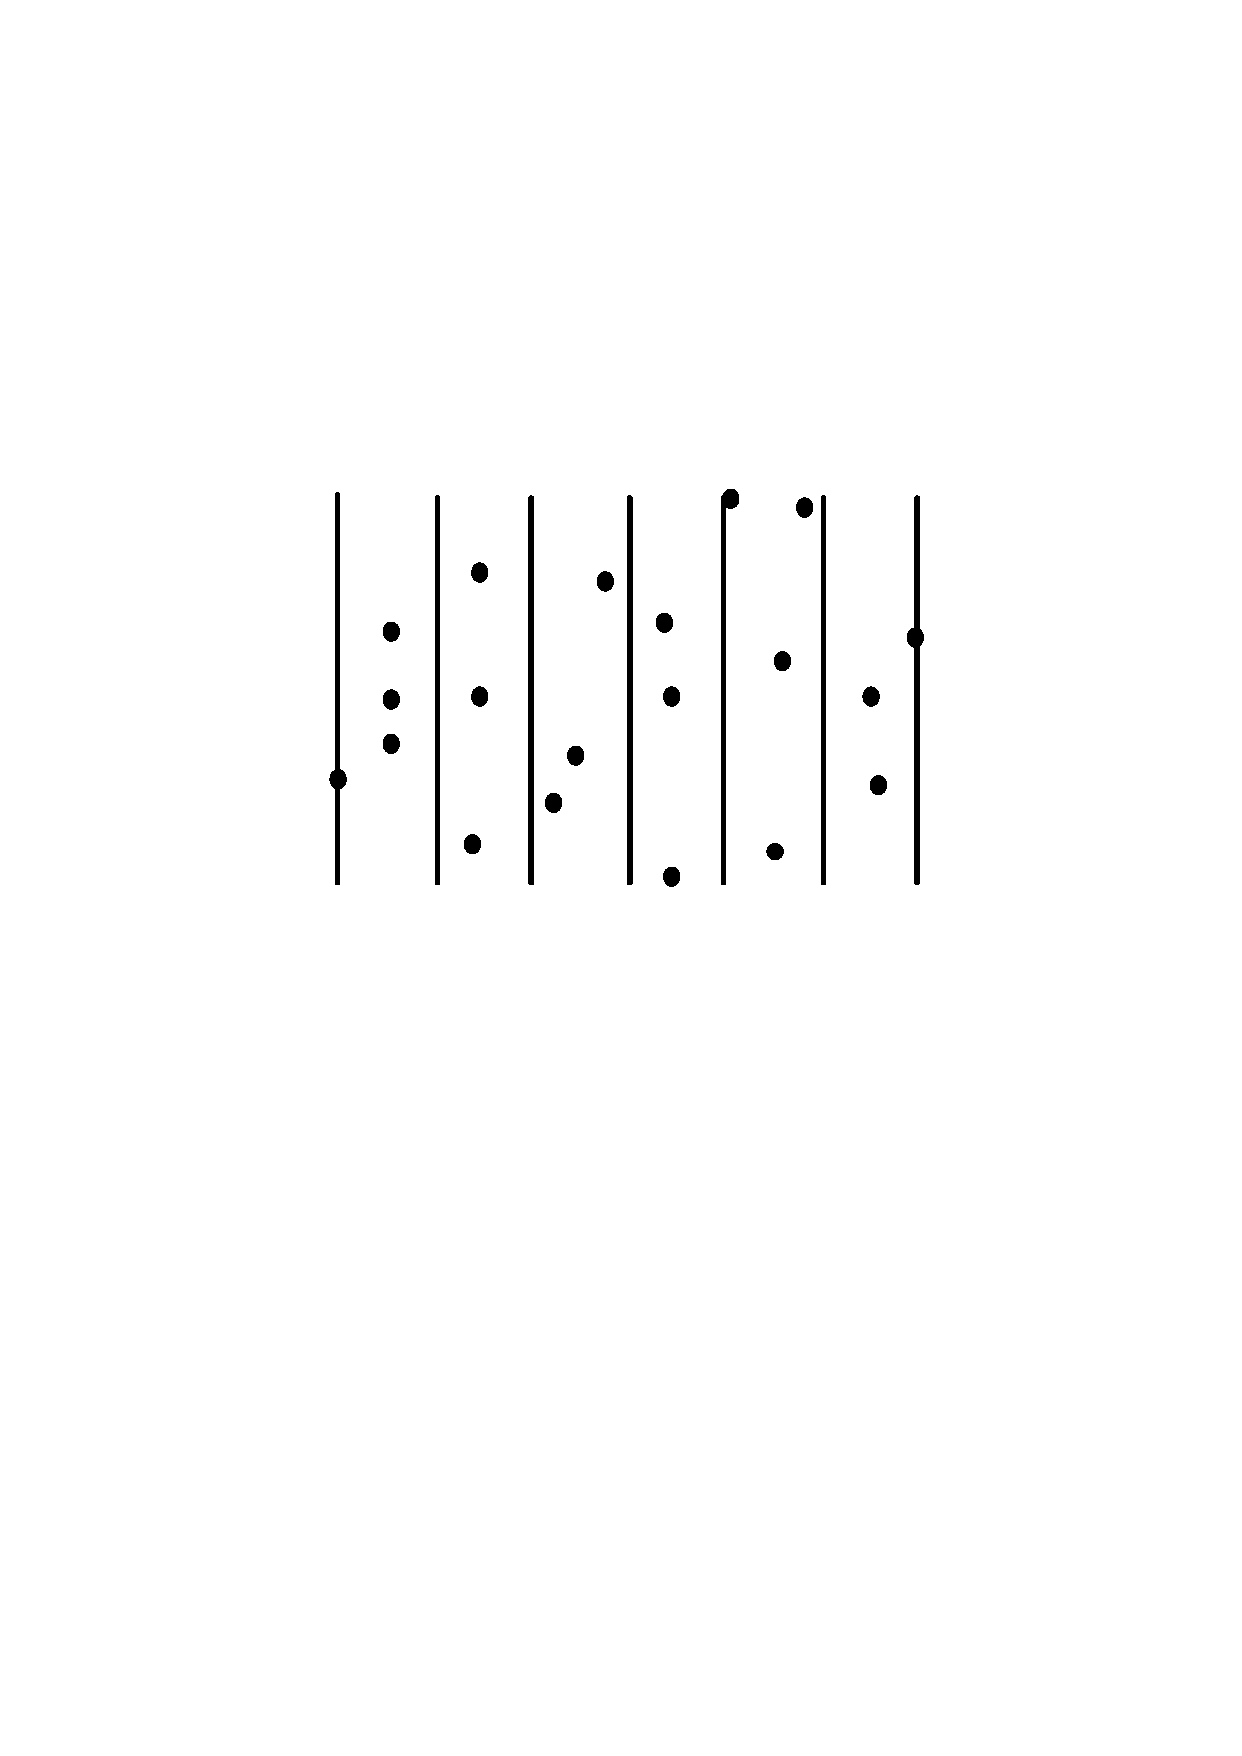
\includegraphics[width=2.2in]{approximate-convexhull-step1.pdf}} \hspace{0.5cm}
  \linebreak
  \subcaptionbox{选极值点\label{lbl:subfig-find-extrems}}{%
    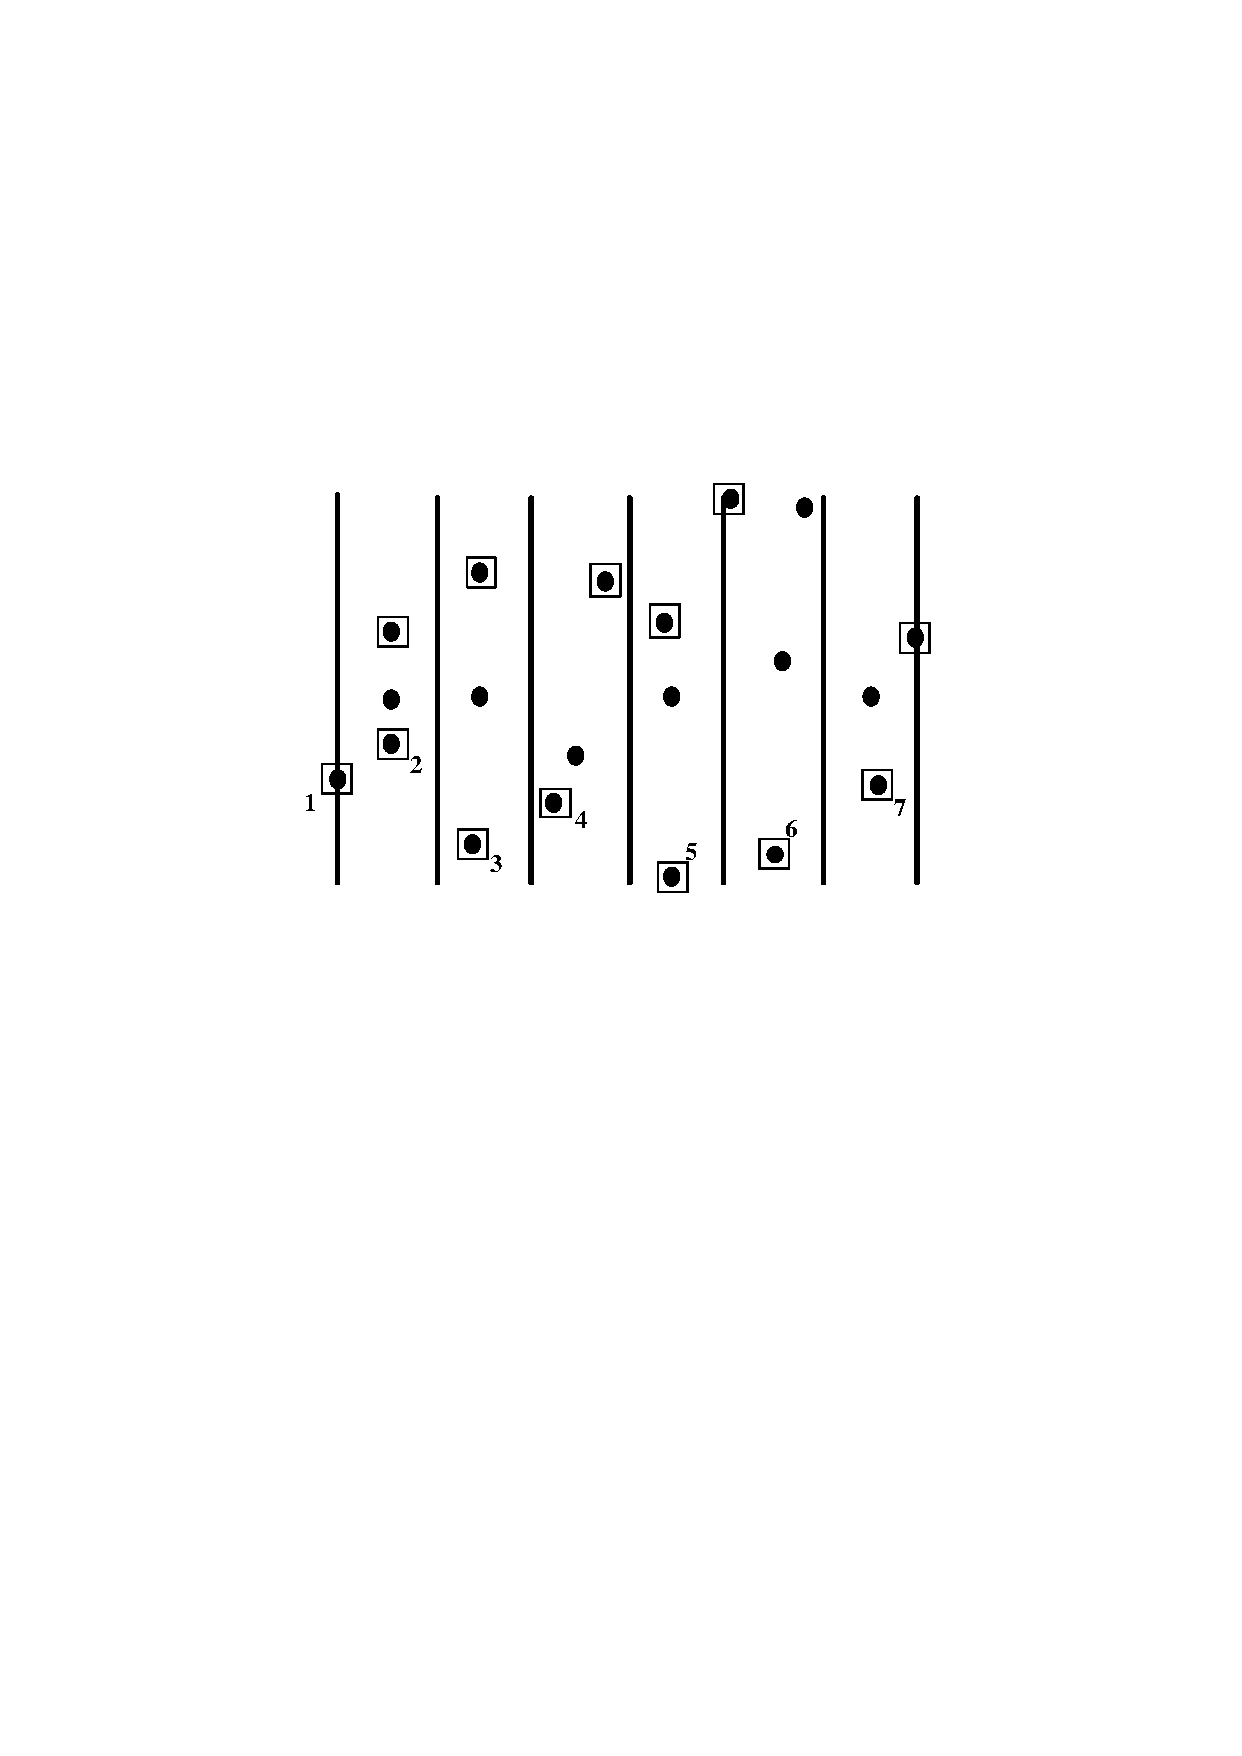
\includegraphics[width=2.2in]{approximate-convexhull-step2.pdf}} \hspace{0.5cm}
  \hspace{2em}
  \subcaptionbox{连线\label{lbl:subfig-connect-extremes}}{%
    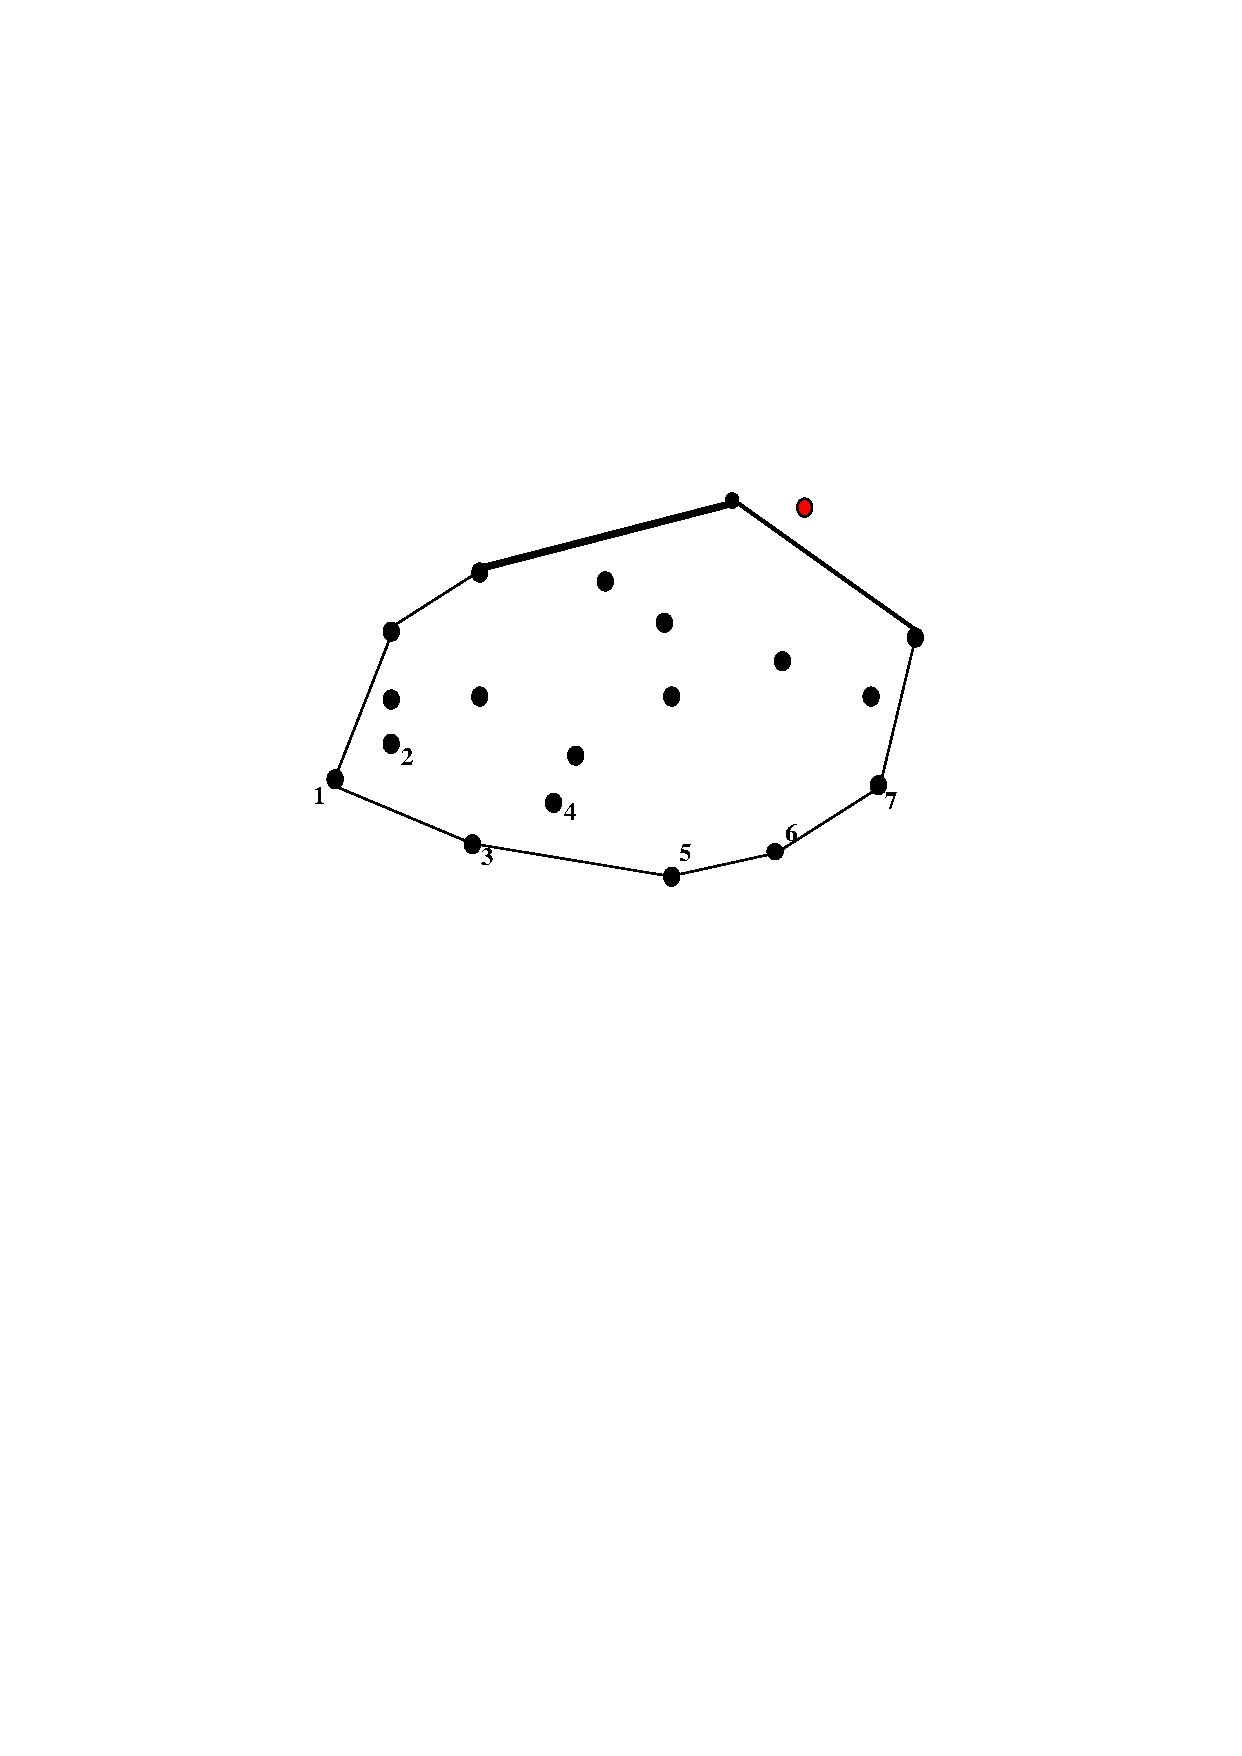
\includegraphics[width=2.2in]{approximate-convexhull-step3.pdf}} \hspace{0.5cm}
  \caption{二维近似内凸包的构造\cite{bentley1982approximation}}
\label{lbl:ach-2d}
\end{figure}

如图~\ref{lbl:ach-2d}~所示,整个算法分为如下3个步骤:

\begin{inparaenum}[(1)]
%\begin{enumerate}[(1)]
\item \textbf{分组:}
首先根据~$x$~轴将输入点集均分~$\xi$~组,如图~\ref{lbl:subfig-split-groups}所示,$\xi$值可以根据输入点集数量以及希望得到的近似凸包的近似程度进行选取,图示中分成了~6~组。\\
\indent \item \textbf{选极值点:}
然后在每组中找出沿~$y$~轴的最大最小坐标值的点,得到每组的极值点,如图~\ref{lbl:subfig-find-extrems}~所示,在边界上的点可直接当作极值点。\\
\indent \item \textbf{连线:}
最后按条件连接每组的最值构成近似内凸包,如图~\ref{lbl:subfig-find-extrems}所示,以下半圈为例,在选定的极值点中先选定最左边的点~1,下一个候选点~2,连接~13~发现候选点~2~在~13~的左边,丢弃候选点~2~直接连接~13,同理连接~35,
当查看候选点~6~时,发现点~6~在~57~连线的右边,因此候选点~6~保留,依次类推可得整个下半圈为凸包,上半圈同理可得。最后合并上下半圈得到如图~\ref{lbl:subfig-connect-extremes}所示的结果。
\end{inparaenum}
%\end{enumerate}

此算法复杂度为~$O(n+\xi)$。  
得到近似凸包后,因较长的边(图~\ref{lbl:subfig-connect-extremes}~中的粗边)对最后凸包围多边形影响较大, 因此可以保留较长的~$a$~条边, 其他~$n-a$($n$~为近似内凸包边数)进行聚类得到~$k-a$~类, 最后得到边对应的垂直向外的方向作为法向。
在三维空间里, 可按照~$x,y$~轴最多划分成~$(\xi+2)\times (\xi+2)$~个正方体网格, 每个正方体网格取~$z$~轴的最大最小坐标值, 因此所有网格含最多含有~$2(\xi+2)^2$~个极值点, 其凸包可以在~$O(\xi^2\log \xi^2) = O(\xi^2\log \xi)$~内求得, 因此整个算法时间复杂度为~$O(n+\xi^2\log\xi)$, 
关于此算法更详细的细节可参考文献~\onlinecite{bentley1982approximation}。 实验过程中, 为了更快地构造近似内凸包, $\xi$~值通常取得较小(例如取~$\xi=10$)。

假设点~$A,B,C$~为近似凸包的某个平面~$P_i$~上逆时针方向上的3个顶点,则该平面~$P_i$~的法向~$\bm{n_i}
= \overrightarrow{AB} \times
\overrightarrow{AC}$,这些法向就是参与聚类算法的所有样本法向集。

\subsection{聚类初始点的选择}
\label{subsec:initial-normals}

聚类算法是数据挖掘领域里的研究热点之一,$k$-means~是最流行和最简单的基于划分的聚类算法\cite{Jain2010}。其中,$k$-means
算法最初的步骤就是初始聚类中心的选择。本文算法将采取如下的策略生成:给定一个单位球,将其按照等面积划分成$k$份即$k$-means中的参数$k$,连接球心到每份中心点构成的方向作为法向,其效果如图~\ref{lbl:kmeans-init-normals-26}~所示($k=26$)。

\begin{figure}[htbp]
    \centering
    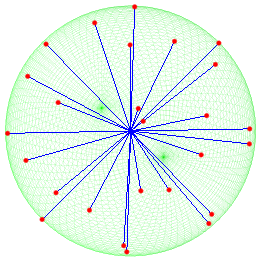
\includegraphics[height=1.7in]{kmeans-init-normals-26.png}
    \caption{初始聚类法向的生成}
    \label{lbl:kmeans-init-normals-26}
\end{figure}
初始点生成算法具体如算法~\ref{alg:get_init_normals_by_area}~所示\footnote{http://www.cmu.edu/biolphys/deserno/pdf/sphere\_equi.pdf}。
另外,亦可使用如文献~\onlinecite{wong1997sampling}~中的数学统计方法在球面上生成若干个点使其满足均匀分布。

\begin{algorithm}[htbp]
\small
\caption{初始法向的生成}
\label{alg:get_init_normals_by_area}
\begin{algorithmic}[1]
\Require
初始法向数量~$k$
\Ensure
$k$~个法向~$normals$

\Function{GenerateInitNormal}{$k$}
  \State $area \leftarrow 4\pi / k$
  \State $m\_v \gets \Call{round}{\pi/\sqrt{area}}$
  \State $d\_v \gets \pi/m\_v$
  \State $d\_phi \gets area/d\_v$
  \For {$m=0 \to m\_v-1$}
      \State $v \gets \pi m/m\_v$
      \State $m\_phi \gets \Call{round}{2\pi\sin{v}/d\_phi}$
      \For {$n=0 \to m\_phi-1$}
          \State $\phi \gets 2\pi n/m\_phi$
          \State $normals \gets normals \cup \Call{vec3}{\sin{v}\cos{\phi},\sin{v}\sin{\phi},\cos{v}}$
      \EndFor
  \EndFor
  \State \Return $normals$
  \EndFunction
\end{algorithmic}
\end{algorithm}
 
\subsection{聚类确定法向}
\label{subsec:determ-normals}

聚类算法将相似程度高的变量聚集到一类,距离度量是$k$-means中的关键,采用不同的距离计算函数可能得到不同的聚类结果,依据数据的不同性质可选用不同的距离度量方法,常用的有欧式距离,曼哈顿距离和卡方距离等等。
本文采用余弦距离度量,将方向相近的点归聚到一类。$k$-means~本质上是一个迭代贪心算法,每一次迭代需要重新计算每一类的中心点,直到两次迭代后中心点相差在给定的容差范围内为止。
完整的算法如算法~\ref{alg:kmeans-determine-normals}~所示。

\begin{algorithm}
\small
\caption{$k$-means~确定法向}
\label{alg:kmeans-determine-normals}
\begin{algorithmic}[1]
\Require
初始中心点~$init$, 聚类数量~$k$, 聚类样本法向集~$points$
\Ensure
~$k$~个聚类后的法向 $result$
\Function{kmeansCluster}{$init, k, points$}
  \ForAll {$p \in points$}
    %\State $tmp \gets -\infty $
    \ForAll {$c \in init$}
        \State $\phi \gets c \cdot p$ \Comment{计算余弦距离, 并记录每个聚类变量属于哪一类}
        %\State $tmp \gets max(tmp, \phi)$ \Comment{记录每个聚类变量属于哪一类}
    \EndFor
    \ForAll {$c \in init$}
    \State $result \gets \Call{Update}{c}$ 
        \Comment{按照公式(\ref{equ:kmeans-update-center})更新中心点}
        \State \Comment{检测继续迭代条件是否满足,中心点容差范围内不再变化或迭代次数超过最大迭代次数}
        \If{$ \Call{checkState}{result, init, iter}$}
        \State \Return {$result$}
    \Else
        \State $init \gets result $
        \State $iter \gets iter+1 $
    \EndIf
    \EndFor
  \EndFor
\EndFunction
\end{algorithmic}
\end{algorithm}

算法~\ref{alg:kmeans-determine-normals}~中第7行~\textproc{Update}~方法作用是聚类迭代更新每类的中心点,
本文更新中心点时将每个法向对应的面片的面积作为权重即
\begin{equation}
\label{equ:kmeans-update-center}
\bm{c_i}=\frac{\sum_{i=1}^{i=n} \omega_i \cdot \bm{n_i} } {\sum_{i=1}^{i=n} \omega_i}
,
\end{equation}
其中,$\bm{c_i}$~为第~$i$~类的中心点,$\omega_i$~为法向~$\bm{n_i}$~所在面片对应的面积,这样使得生成的法向尽量靠近原始近似凸包面积较大的面片的方向。

通过用聚类方法得到的法向生成的凸包围多面体比直接用初始法向生成的包围体更加紧致。
如图~\ref{lbl:kemans-fixed-kcbp}~所示, 
其中图~\ref{lbl:fixed-kcbp-bunny}~为按照初始方向为~Bunny~模型生成的凸包围多面体,其中~$k=26$。
聚类后其法向及其生成的凸包围多面体如图~\ref{lbl:kmeans-kcbp-bunny}~所示,后者的紧致程度比前者高~14.98\%。

\begin{figure}[htbp]
\setcounter{subfigure}{0}
  \centering
  \subcaptionbox{初始法向生成$k$-CBP\label{lbl:fixed-kcbp-bunny}}{%
    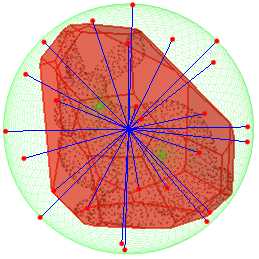
\includegraphics[width=1.8in]{kmeans-init-normals-26-for-bunny.png}}\hspace{3em}%
  \subcaptionbox{聚类法向生成$k$-CBP\label{lbl:kmeans-kcbp-bunny}}{%
    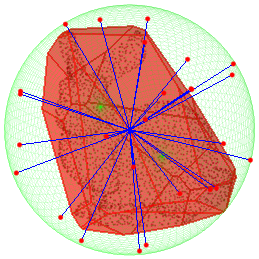
\includegraphics[width=1.8in]{kmeans-cluster-normals-26-for-bunny.png}}\hspace{3em}%
  \caption{初始法向和聚类确定法向生成$k$-CBP对比($k=26$)}
  \label{lbl:kemans-fixed-kcbp}
\end{figure}

\section{搜索截面}
\label{sec:search:planes}

在确定构成~$k$-CBP~的法向后,只需要搜索空间上的一个点即可确定
~$k$-CBP~的截面,搜索截面等效于寻找沿着法向上的最大投影值,即对每个法向~$\bm{n_i}$,从输入模型的所有点中寻找最大投影值的点作为切点进而确定法向~$\bm{n_i}$~对应的截面。
具体算法如算法~\ref{alg:search-plans-cpu}~所示,算法输入为第~\ref{sec:gen-normals}得到的截面法向~$normals$~和模型所包含的点集$points$,算法结束返回多面体的截面~$planes$,
每个截面都是由法向和沿该法向上最大投影值的点构成的,该过程的时间复杂度为~$O(k\cdot n)$,其中~$k$~为法向数量,$n$~为模型点的数量。

\begin{algorithm}[htbp]
\small
\caption{搜索截面串行算法}
\label{alg:search-plans-cpu}
\begin{algorithmic}[1]
\Require
截面法向~$normals$, 模型点集~$points$
\Ensure
多面体截面 $planes$
\Function{SearchCuttingPlanes}{$normals, points$}
  \ForAll {$\bm{n} \in normals$}
      \ForAll {$\bm{p} \in points$}
          \State $proj \gets  \bm{p} \cdot \bm{n}$ \Comment{计算投影值}
          \State $max\_proj \gets \Call{max}{proj, max\_proj}$ \Comment{更新最大投影值}
      \EndFor
  \EndFor
  \ForAll {$\bm{n} \in normals$}
      \State $max\_point \gets \bm{n} \cdot max\_proj$ \Comment{切点}
      \State $planes\gets planes \cup \Call{plane}{\bm{n}, max\_point}$ \Comment{构造平面}
  \EndFor
  \State \Return $planes$
\EndFunction
\end{algorithmic}
\end{algorithm}

从算法~\ref{alg:search-plans-cpu}~可以看出该搜索过程中各法向的计算相互独立,互不影响,因此可方便地借助~GPU~并行加速。
本文将采用着色器和基于~GPU~的通用计算框架两种较流行的并行平台进行~GPU~加速,具体而言为基于~OpenGL~着色语言和~CUDA~框架,下面将分别介绍这两种平台的实现。

\subsection{基于着色器的并行算法}
\label{subsec:determ-normals-by-shader}

OpenGL~提供了可编程管线,它的轻便性、跨平台性和被广泛硬件厂家所支持使得~OpenGL~着色语言(OpenGL Shading Language,简称~GLSL)被广泛应用,在基于~GPU~的通用计算(General
Purpose Graphic Process Unit,简称~GPGPU)中也发挥着重要作用。下面将分别介绍本文提出的基于深度缓冲(Z Buffer)和乒乓技术的算法。

\subsubsection{基于深度缓冲的算法}
	
在~OpenGL~中,当渲染~3D~模型时,深度测试是在片段着色器工作后的一个重要测试操作,当两个片段在相同的位置时,深度测试的目的是决定哪个片段将要保留下来,默认情况下,最前面即有较小(或较大,可设置)的~$z$~坐标值的片段将通过测试被保留下来。
每个片段的深度信息保存在深度缓冲中,当新的片段通过测试后将更新缓冲中的值。
本文充分利用了~OpenGL~的这种机制,算法每走一遍渲染流程将找出一个方向上的切点,在顶点着色器中,将所有点的~$x,y$~坐标值设为一样,并将该点在法向上的投影作为~$z$~值即深度值,所有点经过深度测试后将只有~$z$~值最大的点被保留下来,该点就是沿着这个法向的切点。该过程的算法流程图如~\ref{fig:flowchart:zbuffer}~所示。

\begin{figure}[htbp]
  \centering
  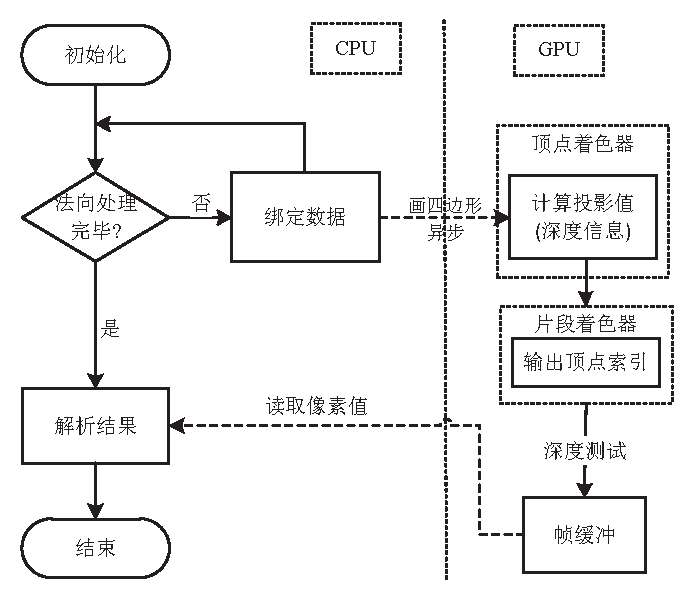
\includegraphics[width=4.0in]{shader-z_buffer.eps}
  \caption{基于~Z Buffer~算法流程图}
  \label{fig:flowchart:zbuffer}
\end{figure}

在实际实现过程中需要注意默认情况下~OpenGL~处理~$x$~和~$y$~坐标值的范围是~$[-1,1]$,而深度值需要映射到~$[0,1]$。我们利用一张~$k \times 1$~大小的纹理保存结果,将第~$i$~个法向的切点保存在纹理的~$(i,0)$~坐标处,
这样做的好处是每绘制一遍不用清除深度缓冲,最后可以一次性读取这个~$k \times 1$~大小的纹理得到结果。
如代码~\ref{shader:zbuffer}~的着色器代码所示,OpenGL~中利用齐次坐标处理渲染流程,因此我们利用前三个分量保存法向的~$x,y,z$~坐标值,第4个分量~$w$~保存法向的索引,在片段着色器中,只需要简单地输出切点的在输入点数组的索引即可。
通过绘制~$k$~遍,我们从大小为~$k \times 1$~的纹理中读出点索引以此就能确定~$k$~切平面,每绘制一遍得到1个切平面,当~$k$~值较大时,这个过程仍然比较耗时,从实验结果也能看出,这种算法适用于~$k$~值相对较小的情况。
%\lstinputlisting[language={shader}, caption={Vertex shader(Z buffer algorithm)}, label=vertex_shader_zbuffer]{shader_zbuffer.vert}
\lstinputlisting[language={shader}, caption={基于~Z Buffer~算法着色器代码}, label=shader:zbuffer]{shader_zbuffer.vert}

\subsubsection{基于乒乓技术的算法}

渲染到纹理(Render To Texture,简称~RTT)是一个非常重要的图形可视化技术,它能够帮助快速地渲染很多漂亮的结果,同时也是~GPGPU~重要组成部分。在基于~OpenGL~的~GPGPU~中,通常要将参与计算的数据通过~CPU~传送至~GPU~的特定大小的纹理中,
通过绘制一个与保存数据有着同样大小的四边形来调用着色器中的算法\cite{gpgpuqiu},将结果输出到纹理中。该过程中,绘制同样大小的四边形是为了避免纹理插值对输入数据的影响。
RTT~的算法一般是在片段着色器(Fragment Shader)中完成,有时通过一遍的绘制得不到最终结果还需要把前一次运算结果传递给下一次运算用来作为后继运算的输入,此时可以利用乒乓技术来解决。

\begin{figure}[htbp]
  \centering
  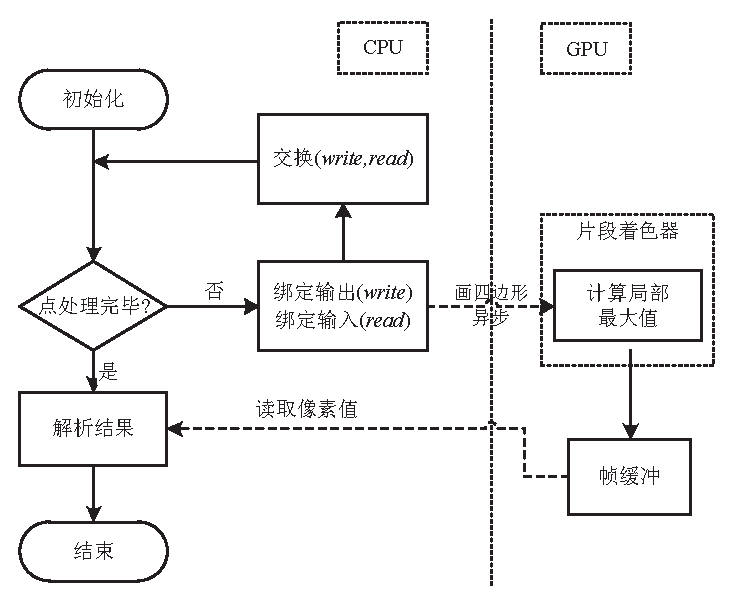
\includegraphics[width=4.2in]{shader-rtt_pp.eps}
  \caption{基于乒乓技术算法流程图}
  \label{fig:shader-rtt-pingpong-flowchart}
\end{figure}

图~\ref{fig:shader-rtt-pingpong-flowchart}~为基于乒乓技术的算法的流程图,算法将所有法向保存在纹理~$read$~中并利用纹理~$write$~缓存中间结果,第~$m$~次渲染进行计算时,纹理~$read$~作为输入,将渲染即计算的结果缓存在纹理~$write$~中,
在第~$m+1$~次渲染时将读取缓存在纹理~$write$~中的数据作为输入,而此时纹理~$read$~又作为输出,如此进行交替,每步交换只更改沿着每个法向的局部最大值。
如代码~\ref{shader:pingpong}~中的片段着色器代码所示,用一个像素值保存法向的~$xyz$~坐标值和沿着该法向投影得到最大值,另外该像素的第四个分量保存该最大值点在输入点数组中的索引。
算法将输入点分成~$x$~份,每次只处理一份,在当前渲染过程中,找出在该批点集中沿着所有法向投影值最大的点,当处理下批点集即下一次渲染时,将与上次局部最大投影值进行比较,若有新的投影最大值就更新,如此反复~$x$~次,
当所有点都被处理完毕后得到沿着所有法向投影最大值的点即切点。最后再通过~CPU~一次性从帧缓冲中读取所有法向的切点。
\lstinputlisting[float=!ht, language={shader}, caption={基于乒乓技术算法着色器代码}, label=shader:pingpong]{shader_rrt_pingpong.frag}

与~Z Buffer~算法相比,基于乒乓技术的算法在进行一次绘制操作能够得到沿着~$k$~个法向的局部(所有处理过的点集)最大值。为了充分利用~GPU~的并行计算能力,将每次处理点的数量设置为~GPU~硬件所支持的~OpenGL~中统一块(uniform
block)所能容纳数据的大小,即需要反复绘制的次数为~$x=n/b$,其中~$n$~为点集大小,$b$~为统一块能容纳点的数量,值与显卡具体型号有关。 

\subsection{基于~CUDA~的并行算法}
\label{subsec:determ-normals-by-cuda}

~CUDA~是显卡公司~NVIDIA~推出的通用的并行计算架构平台,能够利用~GPU~解决并行计算问题,并提供了多种语言的编程接口。
CUDA~程序可以由一系列的主机程序组成,主机程序能够并行地在~GPU~设备上运行,GPU~运算单元将并行的线程分解成线程块,每个线程块又由若干线程组成,GPU~的流水处理器以线程块为单位进行调度。
将问题划分成子问题提交给~GPU~让多线程同时处理这些子问题,这样可以提升算法的效率\cite{lauterbach2009fast}。

如图~\ref{lbl:reduction-getmax}~所示,最大投影值的计算可采用如下规约方式:将输入点交给数量为~$t$~的线程计算点积得到投影值,
线程~$i$~和~$i+t/2$~比较选取较大者,经~$\log_2t$~次比较可得最大值。
这种规约方式也很容易移植到开放计算语言(Open Computing Language,简称~OpenCL)等并行计算框架平台上\cite{gpgpuqiu},在此不再赘述。

\begin{figure}[htbp] % use [htbp] to fix the position
\centering
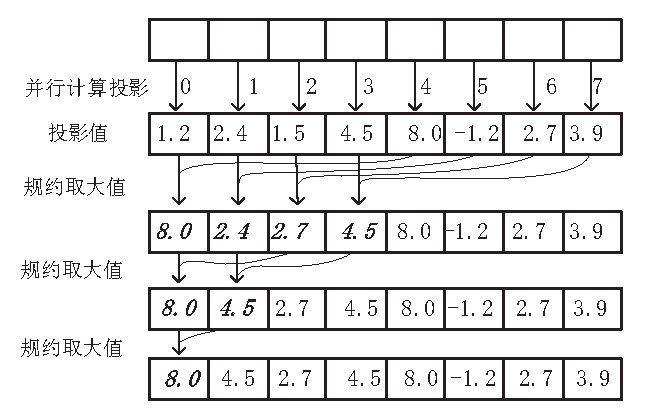
\includegraphics[width=4.2in]{gpureduction.eps}
\caption{并行规约求最大投影值}
\label{lbl:reduction-getmax}
\end{figure}

图~\ref{lbl:reduction-getmax}~所示的示例中,假设有~8~个点与某法向点积得到的投影值为~$(1.2,2.4,1.5,4.5,8.0,-1.2,2.7,3.9)$,有4个线程~同时比较第~$i$~个投影值与~$i+4$~投影值得到新的较大投影值~$(8.0,2.4,2.7,4.5)$,并将新的较大的投影值放入线程~$i$~中,
再以同样的方式规约得到较大的两个投影值~$(8.0,4.5)$,最后再通过一次比较得到最大的投影值~$8.0$~。
文献~\onlinecite{Harris2007Optimizing}介绍了更多更详细规约优化技术。

\section{截面求交算法}
\label{sec:intersect-planes}

确定~$k$-CBP~各个截面后,直接求得所有平面的交点并排除在平面外部的交点即可得到~$k$-CBP~的顶点。该问题即转化为:给定~$k$~个平面及其法向,平面及法向相当于一个半空间~$\bm{H}$,即已知集合$\{\bm{H_1},
\bm{H_2}, \cdots, \bm{H_k}\}$,求$\bm{H_1} \cap \bm{H_2} \cap \cdots
\cap \bm{H_k}$。该问题是一个线性规划(Linear Programming)问题,文献~\onlinecite{dengcg}~详细介绍了在二维线性规划下的相关算法,本文将分别介绍一种直观的枚举算法和利用对偶映射的方法求得~$k$-CBP~的交点。

\subsection{枚举法}
\label{subsec:intersection-enum-geometry}

空间中的平面位置情况如图~\ref{fig:three-planes-intersection}~所示,可分为如下几种情况:
\begin{inparaenum}[(1)]
\item \textbf{无交点},若3个平面互相平行则没有交点,如图~\ref{lbl:intersection-center-0}~所示;
\item \textbf{1~条交线}, 如图~\ref{lbl:intersection-center-1}~所示,3个平面相交于~1~条交线;
\item \textbf{2~条交线}, 当有两个平面互相平行,另一个平面与其相交时有2条交线,如图~\ref{lbl:intersection-center-2}~;
\item \textbf{3~条交线}, 如图~\ref{lbl:intersection-center-3}~所示,3个平面交于~3~条交线;
\item \textbf{1~个交点}, 最后一种情况是三个平面相交于1点的情况,如图~\ref{lbl:intersection-center-4}~所示。
\end{inparaenum}

一个凸多面体的每一个顶点都可看作是至少3个平面的交点。现在只需要枚举出所有3个平面相交于1点的所有情况即可得到$k$-CBP~的顶点,值得注意的是,并非所有交点都是多面体的顶点,交点在某个半空间的正方向上即在半空间相交区域的外部须排除。

\begin{figure}[htbp]
  \centering
  \subcaptionbox{没有交点\label{lbl:intersection-center-0}}{%
    
\includegraphics[width=1.8in]{intersection-center-0.png}}\hspace{1em}%
  \subcaptionbox{交于~1~条线\label{lbl:intersection-center-1}}{%
    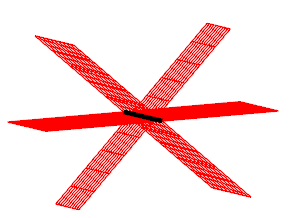
\includegraphics[width=1.8in]{intersection-center-1.png}}\hspace{1em}%
  \subcaptionbox{交于~2~条线\label{lbl:intersection-center-2}}{%
    
\includegraphics[width=1.8in]{intersection-center-2.png}}%
  \\
  \subcaptionbox{交于~3~条线\label{lbl:intersection-center-3}}{%
    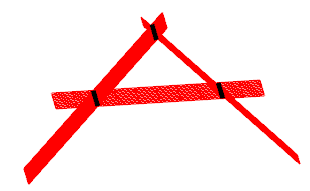
\includegraphics[width=2.3in]{intersection-center-3.png}}%
  \subcaptionbox{交于~1~个点\label{lbl:intersection-center-4}}{%
    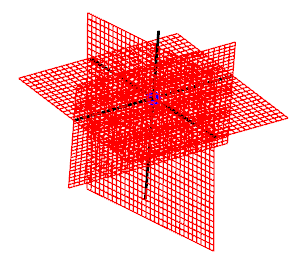
\includegraphics[width=2.0in]{intersection-center-4.png}}%
  \caption{空间中~3~个平面的相交情况}
  \label{fig:three-planes-intersection}
\end{figure}

假设满足如图~\ref{lbl:intersection-center-4}~所示的三个平面的法向分别是$\bm{n_1}, \bm{n_2}, \bm{n_3}$,
平面上一点分别为~$\bm{p_1}, \bm{p_2}, \bm{p_3}$,则三个平面的交点须满足如下方程: 
\begin{equation}
  \label{equa:three-planes-intersection}
  \left\{
    \begin{array}{l}
      \bm{n_1} \cdot \bm{x} = \bm{n_1} \cdot \bm{p_1}\\
      \bm{n_2} \cdot \bm{x} = \bm{n_2} \cdot \bm{p_2}\\
      \bm{n_3} \cdot \bm{x} = \bm{n_3} \cdot \bm{p_3}
    \end{array}
    \right.
\end{equation}

令$(\bm{n_1} \cdot \bm{p_1}, \bm{n_2} \cdot \bm{p_2}, \bm{n_3} \cdot \bm{p_3})
= (y_1, y_2, y_3) = \bm{y}$,则求解式(\ref{equa:three-planes-intersection})相当于解线性方程组
$\bm{A} \bm{x}=\bm{y}$ 即 $(\bm{n_1},\bm{n_2}, \bm{n_3})^T \cdot \bm{x} = \bm{y}$, 令
$\bm{n_i} = (a_{i1}, a_{i2}, a_{i3}), i=\{1,2,3\}$,则有:
\begin{equation*}
  \label{equa:matrix:crammer}
  \left(
    \begin{array}{ccc}
      a_{11} & a_{12} & a_{13} \\
      a_{21} & a_{22} & a_{23} \\
      a_{31} & a_{32} & a_{33} \\
    \end{array}
  \right)
  \cdot 
  \bm{x} 
 % \left(
 %   \begin{array}{c}
 %     x_{1} \\
 %     x_{2} \\
 %     x_{3} \\
 %   \end{array}
 % \right)
  =
  \left(
    \begin{array}{c}
      y_{1} \\
      y_{2} \\
      y_{3} \\
    \end{array}
  \right)
\end{equation*}

根据克莱姆法则(Crammer's Rule),上述方程有唯一解,则
$|\bm{A}| \not= 0$,且解~$x_i = \frac{|\bm{A_i}|}{|\bm{A}|}, i =
\{1,2,3\}$,其中~$|\bm{A}_i|$~是矩阵~$\bm{A}$~中将第~$i$~列替换成~$\bm{y}^T$~之后的行列式,在计算~$\bm{A}_i$~和~$|\bm{A}|$~时为了避免一些重复计算,将其展开有:
\begin{equation*}
 \left\{
\begin{array}{llll}
%\begin{aligned}
    |\bm{A}|   &=
    a_{11}  \left|
                  \begin{array}{cc}
                    a_{22} & a_{23} \\
                    a_{32} & a_{33} \\
                  \end{array}
              \right|
    &- a_{12} \left|
                  \begin{array}{cc}
                    a_{21} & a_{23} \\
                    a_{31} & a_{33} \\
                  \end{array}
              \right|
    &+ a_{13}
              \left|
                  \begin{array}{cc}
                    a_{21} & a_{22} \\
                    a_{31} & a_{32} \\
                  \end{array}
              \right|
\vspace{0.5em}\\ \vspace{0.5em}
    |\bm{A}_1| &= 
    y_1     \left|
                  \begin{array}{cc}
                    a_{22} & a_{23} \\
                    a_{32} & a_{33} \\
                  \end{array}
              \right|
    &- a_{12} \left|
                  \begin{array}{cc}
                    y_2 & a_{23} \\
                    y_3 & a_{33} \\
                  \end{array}
              \right|
    &+ a_{13}
              \left|
                  \begin{array}{cc}
                    y_2 & a_{22} \\
                    y_3 & a_{32} \\
                  \end{array}
              \right|
\\ \vspace{0.5em}
    |\bm{A}_2| &= 
    a_{11}  \left|
                  \begin{array}{cc}
                    y_{2} & a_{23} \\
                   y_{3} & a_{33} \\
                  \end{array}
              \right|
    &- y_{1}  \left|
                  \begin{array}{cc}
                    a_{21} & a_{23} \\
                    a_{31} & a_{33} \\
                  \end{array}
              \right|
    &+ a_{13}
              \left|
                  \begin{array}{cc}
                    a_{21} & y_{2} \\
                    a_{31} & y_{3} \\
                  \end{array}
              \right|
\\ \vspace{0.5em}
    |\bm{A}_3| &= 
    a_{11}  \left|
                  \begin{array}{cc}
                    a_{22} & y_{2} \\
                    a_{32} & y_{3} \\
                  \end{array}
              \right|
    &- a_{12} \left|
                  \begin{array}{cc}
                    a_{21} & y_{2} \\
                    a_{31} & y_{3} \\
                  \end{array}
              \right|
    &+ y_{1}
              \left|
                  \begin{array}{cc}
                    a_{21} & a_{22} \\
                    a_{31} & a_{32} \\
                  \end{array}
              \right|
\end{array}
%\end{aligned}
\right.
\end{equation*}

%TODO 下面可用一个大括号括起来
令
%$b_1 = \left|
%\begin{array}{cc}
%  a_{22} & a_{23} \\
%  a_{32} & a_{33} 
%\end{array} 
%\right|
%  = a_{22}a_{33} - a_{32}a_{23}
%,
%b_2 = \left|
%\begin{array}{cc}
%  a_{21} & a_{23} \\
%  a_{31} & a_{33} 
%\end{array} 
%\right|
%  = a_{21}a_{33} - a_{31}a_{23}
%,
%b_3 = \left|
%\begin{array}{cc}
%  a_{21} & a_{22} \\
%  a_{31} & a_{32} \\
%\end{array}
%\right|
%= a_{21}a_{32}-a_{31}a_{22}
%,
%b_4 = \left|
%  \begin{array}{cc}
%    y_2 & a_{23} \\
%    y_3 & a_{33} \\
%  \end{array}
%\right|
%  = y_2a_{33}-y_3a_{23}
%,
%b_5 = \left|
%  \begin{array}{cc}
%      y_2 & a_{22} \\
%      y_3 & a_{32} \\
%      \end{array}
%    \right|
%  = y_2a_{32}-y_3a_{22}
%,
%b_6 = \left|
%    \begin{array}{cc}
%      a_{21} & y_{2} \\
%      a_{31} & y_{3} \\
%    \end{array}
%  \right|
%  =a_{21}y_{3}-a_{31}y_{2}
%$
\begin{equation*}
  \left\{
    \begin{array}{lll}
        b_1 &= \left|
        \begin{array}{cc}
          a_{22} & a_{23} \\
          a_{32} & a_{33} 
        \end{array} 
        \right|
         &= a_{22}a_{33} - a_{32}a_{23}
        \\
        b_2 &= \left|
        \begin{array}{cc}
          a_{21} & a_{23} \\
          a_{31} & a_{33} 
        \end{array} 
        \right|
          &= a_{21}a_{33} - a_{31}a_{23}
        \\
        b_3 &= \left|
        \begin{array}{cc}
          a_{21} & a_{22} \\
          a_{31} & a_{32} \\
        \end{array}
        \right|
        &= a_{21}a_{32}-a_{31}a_{22}
        \\
        b_4 &= \left|
          \begin{array}{cc}
            y_2 & a_{23} \\
            y_3 & a_{33} \\
          \end{array}
        \right|
         & = y_2a_{33}-y_3a_{23}
        \\
        b_5 &= \left|
          \begin{array}{cc}
              y_2 & a_{22} \\
              y_3 & a_{32} \\
              \end{array}
            \right|
          &= y_2a_{32}-y_3a_{22}
        \\
        b_6 &= \left|
            \begin{array}{cc}
              a_{21} & y_{2} \\
              a_{31} & y_{3} \\
            \end{array}
          \right|
          &=a_{21}y_{3}-a_{31}y_{2}
    \end{array}
\right.
\end{equation*}
则有:
\begin{equation}
  \label{equa:solution:three-planes}
  \left\{
    \begin{array}{lll}
      x_1 =& \frac{|\bm{A_1}|}{|\bm{A}|} =&\frac{y_1b_1-a_{12}b_4+a_{13}b_5}{a_{11}b_1-a_{12}b_2+a_{13}b_3} 
      \vspace{0.5em}\\ \vspace{0.5em}
      x_2 =& \frac{|\bm{A_2}|}{|\bm{A}|} =&\frac{a_{11}b_4-y_{1}b_2+a_{13}b_6}{a_{11}b_1-a_{12}b_2+a_{13}b_3} 
      \\ \vspace{0.5em}
      x_3 =& \frac{|\bm{A_3}|}{|\bm{A}|} =&\frac{-a_{11}b_5-a_{12}b_6+y_{1}b_3}{a_{11}b_1-a_{12}b_2+a_{13}b_3}
    \end{array}
  \right.
\end{equation}其中,$|\bm{A}| \not= 0$。


\begin{algorithm}[htbp]
\small
\caption{截面求交枚举算法}
\label{alg:enum_algortihm}
\begin{algorithmic}[1]
\Require
平面~$planes$
\Ensure
凸包围多面体~$k$-CBP
\Function{ConstructKCBP}{$planes$}
  \ForAll {$p_1 \in planes$}
    \State $Intersection \gets \emptyset $
    \ForAll {$p_2 \in planes$}
          \ForAll {$p_3 \in planes$}
              %\If{$ (p_1 = p_2 || p_1 = p_3 || p_2 = p_3) = \FALSE $}
              \If{$ p_1 \nparallel p_2 \nparallel p_3$}
                  \If{$|A| \not= 0$}
                      \State $P = \Call{vec3}{x_1, x_2, x_3}$
                      \Comment{按照公式(\ref{equa:solution:three-planes})计算得到交点坐标值} 
                      \If{\Call{validate}{P}}
                        \State \Comment{验证交点P是否都在半空间负方向上}
                        \State $Intersection \gets Intersection \cup P$
                      \EndIf
                  \EndIf
              \EndIf
          \EndFor
     \EndFor
     \If {$Intersection.size \geq 3$}
     \State {$k\textrm{-CBP} \gets k\textrm{-CBP} \cup \Call{polygon}{p_1, Intersection}$}
     \Comment{满足条件,加入到结果集}
     \EndIf
  \EndFor
  \State \Return {$k$-CBP}
\EndFunction
\end{algorithmic}
\end{algorithm}

完整的算法如算法~\ref{alg:enum_algortihm}~所示,算法输入为第~\ref{sec:search:planes}节中得到的截面$planes$,输出为~$k$-CBP~,每个~$k$-CBP~的多边形截面由围成多边形的交点和多边形所在平面构成。
算法枚举遍历所有平面的组合,搜索出三个平面交于一点的情况,排除在半空间外部的交点即可得到~$k$-CBP~的顶点,算法复杂度为~$O(k^3)$,此算法思想简单易于理解和实现,但当平面数量较多(即~$k$~值较大)时,会耗费很多时间,与枚举法相比基于对偶映射的算法实现较复杂但其时间复杂度为~$O(k \log k)$,效率更高。

\subsection{对偶映射算法}
\label{subsec:intersection-dual-mapping}

正如~$k$-CBP~的定义所知,$k$-CBP~可看作是多个半空间的交集,一个半空间可由法向$\bm{n}(a,b,c)$及离原点距离~$d$~确定,转换为线性不等式即为
\begin{equation}
  \label{equa:halfspace:defition}
  a_ix+b_iy+c_iz \leq d_i, \quad i=1,2,\cdots,k,
\end{equation}
其中~$a_i,b_i,c_i,d_i$~是不同时为0的实数。

求解~$k$-CBP~可将问题转换为求~$k$~个线性不等式的解。利用对偶映射的方式可在~$O(k \log k)$~的方式解决,
具体方法分为三个步骤\cite{Preparata1985Introduction}:
\\ \indent
\begin{inparaenum}[(1)]
%\begin{enumerate}[(1)]
\item   
首先,将上述线性不等式对偶映射成一个欧式空间上的三维点,
$a_ix+b_iy+c_iz=d_i \rightarrow \bm{p}(-a_i/d_i, -b_i/d_i,-c_i/d_i),d_i \neq 0$,其中~$(a_i,b_i,c_i)$~为第~\ref{sec:search:planes}~节中得到的
截面法向~$\bm{n}$,$d_i=\bm{n} \cdot
max\_point$~为截面法向与截面上的投影点~$max\_point$~的点积,此步骤的算法复杂度为~$O(k)$; \\ \indent
\item
其次,对对偶映射得到的欧式空间~$k$~个点求凸包,此步骤的算法复杂度为~$O(k\log k)$~,可用第~\ref{subsec:convexhull}~节中的分治算法; \\ \indent
\item
  得到凸包后,再利用相同的对偶变换将凸包平面方程映射回欧式空间三维点,这些点即为原始半空间的交点,此步骤的算法复杂度仍为~$O(k)$。
\end{inparaenum}
%\end{enumerate}

综上,该方法总体复杂度为~$O(k\log k)$~。
在利用这种对偶变化时需要注意约束条件即上述不等式中的~$d_i>0$,此时原点~$O(0,0,0)$~始终满足不等式(\ref{equa:halfspace:defition}),体现在算法输入上即原始模型需要包含原点。当原始模型不包含原点时,可以先对模型做一定平移或者也可用另外的对偶变换进行求解,文献\onlinecite{Preparata1979Intersection}对此问题进行了详述的阐述。

\section{实验结果及分析}
\label{sec:exper-kcbp}

本文将针对不同点集规模的模型进行测试\footnote{运行时环境为:Intel(R) Core(TM)
i5-2320 CPU @ 3.2GHz 8G RAM NVIDIA GeForce GTX
650。},从两个角度对生成的~$k$-CBP~进行实验对比,
一方面对生成~$k$-CBP~的速度进行效率上的对比,主要对比了串行算法、基于着色器和~CUDA~环境的并行算法和文献\onlinecite{karlsson2010parallel}的并行算法,其详细结果如~\ref{subsec:exper:efficiency}~节所示;
另一个方面对生成~$k$-CBP~的质量即紧致性上进行了对比实验,主要围绕着凸包、文献\onlinecite{abenchmarking2007}~中实现的~$k$-DOP~进行对比,详细结果见第~\ref{subsec:exper:tightness}~节。

\subsection{凸包围多面体生成效率}
\label{subsec:exper:efficiency}

如图~\ref{fig:chart:exps:cputime}~所示为本文算法(CUDA)与传统的~CPU~算法对比结果,图中横纵坐标分别代表多面体面数和运行时间,其中实线~CPU$\rm{'}$~和$k$-CBP$\rm{'}$分别表示用传统~CPU~方法和本文~CUDA~算法构造凸包围多面体总体耗时,虚线~CPU~和$k$-CBP~分别代表各自算法搜索截面的过程。
从中可以看出,当模型点数量较大时,搜索截面的过程占据了算法绝大多数时间,且随着凸包围多面体的面数~$k$~值增加而线性增长,这与搜索截面时间复杂度~$O(k\cdot
n)$一致,截面求交过程利用第~\ref{subsec:intersection-dual-mapping}~节中的对偶映射法,其时间复杂度为~$O(k\log k)$,
当点数量极大时,如图~\ref{fig:exp:cpu:buggatti}~所示,实线虚线几乎重合即求交等步骤耗时相比整体算法而言几乎可忽略。
当输入模型的点数量越大,本文算法的优势越明显。如~Budda~模型点数量~31k~左右,加速比约为~3 $\sim$ 6~倍,而含有~224k~个点的~Alice~模型和~1010k~个点的~Bugatti~模型,能够加速~7$\sim$9~倍。

\begin{figure}[!ht] % use [htbp] to fix the position
\centering
\subcaptionbox{Budda模型(31232个点)\label{fig:exp:cpu:budda}}
{  
   \includegraphics[width=\fourgraphicswidth\textwidth,page=2]{cudatime.pdf}
}
\subcaptionbox{Dinosaur模型(40277个点)\label{fig:exp:cpu:Dinasour}}
{  
    \includegraphics[width=\fourgraphicswidth\textwidth, page=3]{cudatime.pdf}
}\linebreak %强制换行
\subcaptionbox{Alice模型(224291个点)\label{fig:exp:cpu:alice}}
{  
   \includegraphics[width=\fourgraphicswidth\textwidth, page=4]{cudatime.pdf}
}
\subcaptionbox{Bugatti模型(1010815个点)\label{fig:exp:cpu:buggatti}}
{  
   \includegraphics[width=\fourgraphicswidth\textwidth, page=5]{cudatime.pdf}
}
\caption{基于~CUDA~并行算法运行时间}
\label{fig:chart:exps:cputime}
\end{figure}

图~\ref{fig:chart:exps:shadertime}~为着色器算法根据不同模型构造不同面数的包围体所耗费的时间对比,横坐标表示多面体面数~$k$,纵坐标为运行时间,曲线~cpu、zbuffer和rtt\_pp分别表示基于CPU、深度缓冲(Z Buffer)和基于乒乓技术的算法的运行时间。

\begin{figure}[!ht] % use [htbp] to fix the position
\centering
\subcaptionbox{Apple模型(8118个点)\label{fig:exp:shader:apple}}
{  
   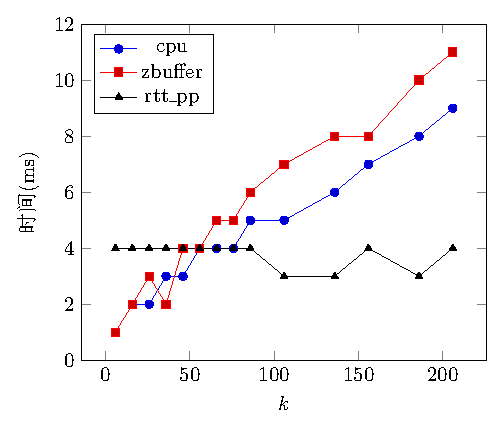
\includegraphics[width=\fourgraphicswidth\textwidth,page=1]{shadertime.pdf}
}
\subcaptionbox{Buddha模型(31232个点)\label{fig:exp:shader:buddha}}
{  
    \includegraphics[width=\fourgraphicswidth\textwidth, page=2]{shadertime.pdf}
}\linebreak %强制换行
\subcaptionbox{Alice模型(224291个点)\label{fig:exp:shader:alice}}
{  
   \includegraphics[width=\fourgraphicswidth\textwidth, page=3]{shadertime.pdf}
}
\subcaptionbox{Bugatti模型(1010815个点)\label{fig:exp:shader:buggatti}}
{  
   \includegraphics[width=\fourgraphicswidth\textwidth, page=4]{shadertime.pdf}
}
\caption{基于着色器的并行算法运行时间}
\label{fig:chart:exps:shadertime}
\end{figure}

从实验结果可以看出,当模型规模不大时,如图~\ref{fig:exp:shader:apple}~所示的含有8千多个点的~Apple~模型,
Z Buffer~算法和传统的~CPU~算法差别不是很大,因此在实际应用中当模型规模较小时可直接用~CPU~计算即可。
随着输入模型所含有点的数量规模的增加,CPU~和~GPU~运行时间之间的差距也越来越大。
当多面体面数增加即~$k$~的增大时,在~Z Buffer~算法中,需要更多的绘制次数,因此其运行时间也有所增加,而在基于乒乓技术的算法中,当点规模一定时,$k$~的变化对最后运行时间影响不明显,因此当较大的~$k$~时,这种算法更快。

\begin{table}[htbp]
\centering
\caption{基于着色器并行算法加速比}
\label{tab:exper:shadertime}
\begin{minipage}[c]{\textwidth}
\begin{center}
  \begin{tabular}{p{1.5cm}<{\centering}cccc cccc} %p本身占一列
  \toprule[1.5pt]
  \multirow{3}{*}{$k$} & \multicolumn{4}{c}{Apple模型(8118 个点)} & \multicolumn{4}{c}{Bugatti~模型(1010815个点)}\\
  \cmidrule(lr){2-5}\cmidrule(lr){6-9}
  & cpu & zbuffer  & rtt\_pp & \multirow{2}{*}{加速比$^{(a)}$} & cpu  & zbuffer& rtt\_pp & \multirow{2}{*}{加速比$^{(a)}$} \\
  & (ms) & (ms)  & (ms) & & (ms)  & (ms) & (ms) \\
  \midrule[1pt]
 6	 & 6 	& 5 	& 41 &	1.20 &	26	& 17	&178  &	1.53 \\
16	 & 16	& 13	& 43 &	1.23 &	70	& 48	&181  &	1.46 \\
26	 & 25	& 17	& 43 &	1.47 &	114	& 68	&183  &	1.68 \\
36	 & 34	& 17	& 45 &	2.00 &	153	& 70	&178  &	2.19 \\
46	 & 44	& 24	& 42 &	1.83 &	203	& 102	&176  &	1.99 \\
56	 & 53	& 31	& 43 &	1.71 &	241	& 131	&177  &	1.84 \\
66	 & 62	& 39	& 43 &	1.59 &	285	& 162	&179  &	1.76 \\
76	 & 73	& 46	& 46 &	1.59 &	331	& 196	&189  &	1.75 \\
86	 & 82	& 52	& 45 &	1.82 &	373	& 225	&192  &	1.94 \\
106	 & 100	& 59	& 45 &	2.22 &	464	& 257	&191  &	2.43 \\
136	 & 127	& 81	& 42 &	3.02 &	604	& 349	&180  &	3.36 \\
156	 & 146	& 88	& 47 &	3.11 &	693	& 378	&202  &	3.43 \\
186	 & 177	& 110	& 43 &	4.12 &	861	& 474	&180  &	4.78 \\
206	 & 194	& 123	& 49 &	3.96 &	962	& 533	&209  &	4.60 \\
  \bottomrule[1.5pt]
\end{tabular}
\end{center}\vspace{-0.5em}
\hspace{1em}
\footnotesize (a): 加速比=~cpu/$min$(zbuffer, rtt\_pp)
\end{minipage}
\end{table}

表~\ref{tab:exper:shadertime}~详细的展示了基于着色器的两种算法应用于~Alice~和~Bugatti~模型的构造时间及相应的加速比。
从中可看出,Z Buffer~算法适合相对较小的~$k$~值,而基于乒乓技术的算法在较大~$k$~值时能达到更大的加速比。

本文实现了文献~\onlinecite{karlsson2010parallel}~中的并行算法并进行对比实验,表~\ref{tab:exp:sse-time}
~为实验统计结果,表中数据均为搜索截面耗时,因为二者其他步骤均相同且从~\ref{fig:chart:exps:cputime}~可得搜索截面时间占用整体绝大部分时间,其中~$k$~为多面体面数,
列~SSE~和列~$k$-CBP~分别为文献~\onlinecite{karlsson2010parallel}~中的算法和本文提出的基于~CUDA~算法的运行时间。

\begin{table}[htbp] 
\centering
\caption{本文算法与文献~\onlinecite{karlsson2010parallel}~的并行算法对比}
\begin{tabular}{p{1.5cm}<{\centering}ccc ccc} %p本身占一列
\toprule[1.5pt]
\multirow{2}{*}{$k$} & \multicolumn{3}{c}{Apple模型(8118个点)} &
\multicolumn{3}{c}{Bugatti~模型(1010815个点)}\\
\cmidrule(lr){2-4}\cmidrule(lr){5-7}
~&SSE\cite{karlsson2010parallel}(ms) & $k$-CBP(ms) &  加速比 & SSE\cite{karlsson2010parallel}(ms) & $k$-CBP(ms) &  加速比\\
\midrule[1pt]
6 & 0.4 & 0.12  & 3.20     & 24.2 & 3.20  & 7.56 \\
16 & 0.9 & 0.26  & 3.43    & 44.5 & 8.44  & 5.27 \\
26 & 1.4 & 0.41  & 3.38    & 66.5 & 13.65  & 4.87 \\
36 & 1.9 & 0.52  & 3.65    & 91.1 & 18.34  & 4.97 \\
46 & 2.5 & 0.67  & 3.74    & 119.5 & 24.13  & 4.95 \\
56 & 2.9 & 0.79  & 3.66    & 138.4 & 28.86  & 4.80 \\
66 & 3.5 & 0.95  & 3.69    & 170.6 & 34.10  & 5.00 \\
76 & 4.0 & 1.08  & 3.70    & 197.1 & 39.85  & 4.95 \\
86 & 4.5 & 1.22  & 3.69    & 219.8 & 45.08  & 4.88 \\
106 & 5.4 & 1.49  & 3.62   & 267.8 & 55.52  & 4.82 \\
136 &  6.8 & 1.92  & 3.54  & 342.9 & 71.24  & 4.81 \\
156 &  7.7 & 2.17  & 3.55  & 411.3 & 81.18  & 5.07 \\
186 &  9.3 & 2.60  & 3.58  & 479.4 & 97.39  & 4.92 \\
206 &  10.5 & 2.85  & 3.68 & 523.0 & 106.87  & 4.89  \\  
\bottomrule[1.5pt]
\end{tabular}
\label{tab:exp:sse-time}
\end{table}

与文献~\onlinecite{karlsson2010parallel}~中的算法相比,本文算法优势明显。
当用于点数量较小~Apple~模型时,能够提高~3$\sim$4~倍速度,模型变大,加速比也更大,~Bugatti~模型的提速达到~4$\sim$8~倍。

\subsection{凸包围多面体紧致程度}
\label{subsec:exper:tightness}

凸包围多面体的质量用公式(\ref{equa:judge:tightness})衡量即通过凸包与凸包围多面体的体积之比来量化包围体的紧致程度。
文献~\onlinecite{abenchmarking2007}~是基于~$k$-DOP~实现的层次结构的包围体,其顶层的~$k$-DOP~与本文算法生成的~$k$-CBP~的紧致程度对比如图~\ref{chart:exps:tightness}~所示,
图中横坐标~$k$~为凸包围多面体的面数,纵坐标为紧致程度,曲线~$k$-DOP~和~$k$-CBP~分别为文献~\onlinecite{abenchmarking2007}~和本文的方法,由图可知,
对于不同模型,本文构造的凸包围多面体紧致程度均有所提升,如~Alice~模型提升了12.08\%,~Dinasour~模型提升了34.0\%。
以~$k \in \{20,38\}$~为例,相应模型的~$k$-DOP~和~$k$-CBP~效果可见图~\ref{fig:kdop:kcbp:ui}。

\begin{figure}[htbp] 
\centering
\subcaptionbox{Apple(8118个点)\label{fix:exp:tightness:apple}}
{
    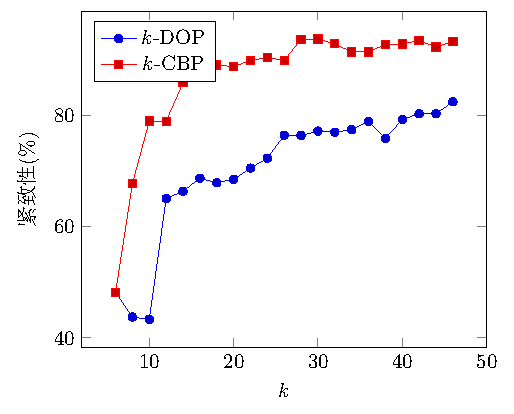
\includegraphics[width=\fourgraphicswidth\textwidth,page=1]{tightness.pdf}
}
\subcaptionbox{Budda(31232个点)\label{fix:exp:tightness:budda}}
{  
   \includegraphics[width=\fourgraphicswidth\textwidth,page=2]{tightness.pdf}
}
\linebreak
\subcaptionbox{Dinosaur(40277个点)\label{fix:exp:tightness:Dinasour}}
{  
    \includegraphics[width=\fourgraphicswidth\textwidth, page=3]{tightness.pdf}
}
\subcaptionbox{Alice(224291个点)\label{fix:exp:tightness:alice}}
{  
   \includegraphics[width=\fourgraphicswidth\textwidth, page=4]{tightness.pdf}
}
\caption{紧致程度对比:$k$-DOP~为文献~\onlinecite{abenchmarking2007}~的算法, $k$-CBP~为本文算法}
\label{chart:exps:tightness}
\end{figure}

\begin{figure}[htbp] 
\centering
\subcaptionbox{Bunny(20-DOP和20-CBP)}
{  
   \includegraphics[width=0.40\linewidth]{bunny-kcbp-dop-20.png}
 }
\subcaptionbox{Bunny(38-DOP和38-CBP)}
{
    \includegraphics[width=0.40\linewidth]{bunny-kcbp-dop-38.png}
}
\linebreak
\subcaptionbox{Apple(20-DOP和20-CBP)}
{  
   \includegraphics[width=0.45\linewidth]{apple-kcbp-dop-20.png}
}
\subcaptionbox{Apple(38-DOP和38-CBP)}
{  
   \includegraphics[width=0.45\linewidth]{apple-kcbp-dop-38.png}
}
\linebreak
\subcaptionbox{Budda(20-DOP和20-CBP)}
{  
   \includegraphics[width=0.40\linewidth]{budda-kcbp-dop-20.png}
 }\hspace{1.5em}
\subcaptionbox{Budda(38-DOP和38-CBP)}
{
    \includegraphics[width=0.40\linewidth]{budda-kcbp-dop-38.png}
}
\linebreak
\subcaptionbox{Dinosaur(20-DOP和20-CBP)}
{  
   \includegraphics[width=0.48\linewidth, height=0.16\linewidth]{dinosaur-kcbp-dop-20.old.eps}
}
\subcaptionbox{Dinosaur(38-DOP和38-CBP)}
{  
   \includegraphics[width=0.48\linewidth, height=0.16\linewidth]{dinosaur-kcbp-dop-38.old.eps}
}
\linebreak
\subcaptionbox{Alice(20-DOP和20-CBP)}
{  
   \includegraphics[width=0.38\linewidth]{alice-kcbp-dop-20.png}
 }\hspace{1.5em}
\subcaptionbox{Alice(38-DOP和38-CBP)}
{
    \includegraphics[width=0.38\linewidth]{alice-kcbp-dop-38.png}
}
\caption{~$k$-CBP~与~$k$-DOP~对比}
\label{fig:kdop:kcbp:ui}
\end{figure}

\begin{table}[htbp]   
\centering
\caption{用近似凸包与精确凸包构造~$k$-CBP~紧致程度对比}
\label{tab:exp:ach:ch:tightness}
\begin{tabular}{lccccl}
\toprule[1.5pt]
$k$ &  $\tau$(ACHull)(\%) & $\tau$ (CHull)(\%)  & $k$ &  $\tau$ (ACHull)(\%) & $\tau$ (CHull)(\%) \\
\midrule[1.0pt]
10 &	70.44 & 	65.56     &26 &	89.93 & 	94.45 \\
12 &	74.56 & 	75.63     &28 &	88.61 & 	92.24 \\
14 &	79.50 & 	82.49     &30 &	91.58 & 	92.35 \\
16 &	84.79 & 	85.20     &32 &	92.78 & 	93.78 \\
18 &	85.75 & 	90.09     &34 &	91.28 & 	93.22 \\
20 &	86.38 & 	90.36     &36 &	92.93 & 	94.68 \\
22 &	90.27 & 	92.48     &38 &	93.41 & 	93.20 \\
24 &	90.70 & 	93.09     &40 &	93.81 & 	94.70 \\
\bottomrule[1.5pt]
\end{tabular}
\end{table}

本文算法利用近似凸包与精确凸包的相似性,从近似凸包的众多面片对应的法向中通过~$k$-means~聚类算法生成~$k$~个法向。
表~\ref{tab:exp:ach:ch:tightness}~为利用~Alice~模型的近似凸包和精确凸包分别聚类生成法向构造~$k$-CBP~的紧致程度对比。
可以看出,一方面,利用精确凸包构造的~$k$-CBP~并不一定比近似凸包构造的结果更紧致,但由于近似凸包与精确凸包的外观的近似性因此二者得到的结果相差并不大(5\%以内);
另一方面,因近似凸包的时间复杂度为线性,而精确凸包为~$O(n\log n)$,
因此本文利用近似凸包聚类生成法向。示例中构造近似凸包耗费时间仅为~0.88ms~,而精确凸包为~79.31ms~。


\begin{table}[htbp] 
\centering
\caption{$k$-CBP~与~QuickHull~凸包算法比较}
\label{tab:exp:cgal}
\begin{tabular}{lcccccl}
\toprule[1.5pt]
 Model & $f$(CHull)& $f$($k$-CBP) & $\tau$ ($k$-CBP)(\%) & $t$(CHull)(ms) & $t$($k$-CBP)(ms)\\ % 后面重新跑的, KCBP加上了近似凸包及求交时间的总和, 和近似凸包的分组时间也加了.
\midrule[1.0pt]
  Apple	& 499 & 30 & 93.67 & 5.5 & 1.30 \\ % apple3  自己电脑跑的数据, 之前是用的chengxianyu的电脑.
  Budda	& 1608 & 46 & 92.39 & 21.3 & 2.86 \\ %  1.0+0.86+1
  Dinosaur	& 1240 & 44 & 93.34 & 22.6 & 1.99 \\  % 1.0+0.98+0.1
  Alice	& 1332 & 44 & 93.92 & 85.8 & 8.47\\ % 2+6.48
  Bugatti & 24654 & 44 & 95.06 & 688.7 & 25.41 \\
\bottomrule[1.5pt]
\end{tabular}
\end{table}

\begin{figure}[!ht] 
\centering
\subcaptionbox{Alice(44-CBP)\label{fig:exp:alice}}
{  
   \includegraphics[width=0.20\textwidth]{alice-44-w-n.png}
}
\subcaptionbox{Apple(30-KCBP)\label{fig:exp:apple}}
{
    \includegraphics[width=0.28\textwidth]{apple-30-w-n.png}
}
\subcaptionbox{Bugatti(44-CBP)\label{fig:exp:buggati}}
{  
  \rotatebox{-80}{\includegraphics[width=0.32\textwidth]{buggati-44-w-n.png}}
}
\subcaptionbox{Budda(46-CBP)\label{fig:exp:budda}}
{  
   \includegraphics[width=0.20\textwidth]{budda-46-w-n.png}
}
\linebreak
\subcaptionbox{Alice(CHull)\label{fig:exp:ch:alice}}
{  
   \includegraphics[width=0.20\textwidth]{alice-convexhull.png}
}
\subcaptionbox{Apple(CHull)\label{fig:exp:ch:apple}}
{
    \includegraphics[width=0.28\textwidth]{apple-convexhull.png}
}
\subcaptionbox{Bugatti(CHull)\label{fig:exp:ch:buggati}}
{  
  \rotatebox{-80}{\includegraphics[width=0.32\textwidth]{bugatti-convexhull.png}}
}
\subcaptionbox{Budda(CHull)\label{fig:exp:ch:budda}}
{  
   \includegraphics[width=0.20\textwidth]{budda-convexhull.png}
}
\linebreak
\subcaptionbox{Dinasour(44-CBP)\label{fig:exp:dinosaur}}
{
    \rotatebox{0}{\includegraphics[width=0.38\textwidth]{dinosaur-44-w-n.png}}
}
\subcaptionbox{Dinosaur(CHull)\label{fig:exp:ch:dinosaur}}
{  
    \rotatebox{0}{\includegraphics[width=0.40\textwidth]{dinosaur-convexhull.png}}
}
\caption{~$k$-CBP~与凸包对比}
\label{pic:exps:ch-kcbp}
\end{figure}


本文算法与~CGAL~库中利用~QuickHull~算法构造的凸包进行比较的结果如表~\ref{tab:exp:cgal}~所示,
其中~$f$(CHull)~和~$f$($k$-CBP)~分别表示凸包的面数和凸包围多面体的面数,$\tau$($k$-CBP)~为凸包围多面体的紧致程度,$t$(CHull)~和~$t$($k$-CBP)~分别表示凸包和~$k$-CBP~构造所花费的时间。
相应模型的可视化结果如图~\ref{pic:exps:ch-kcbp}~所示。
与凸包相比,本文算法在大大简化包围体平面数量的同时能保持较好的紧致程度,例如~Apple~模型的凸包有~499~个平面,本文算法仅用~30~个平面就能达到~93.67\%的紧致程度,
而对~Bugatti~模型,仅用了其凸包平面数量的0.17\%就达到95.06\%的紧致程度,且构造速度快了~27~倍。

\FloatBarrier
\section{本章小结}
\label{sec:chap02:summary}

本章主要介绍了凸包围多面体~$k$-CBP~的生成算法,算法主要分为3个步骤,
首先确定生成的~$k$-CBP~的法向,为了得到更加紧致的凸包围多面体,本文利用~$k$-means~对构造的近似内凸包的法向进行聚类;
然后多次扫描模型点集得到每个法向的切点进而得到截面,该过程各方向计算相互独立互不影响,因此利用了~GPU~进行加速;
最后通过截面求交得到~$k$-CBP~的各个顶点。
本章最后通过实验从凸包围多面体的生成效率和紧致程度两个角度与现有算法进行对比,说明本文算法能够快速构造更加紧致的凸包围多面体,较现有算法相比效率上平均能够提高~3 $\sim$ 8~倍,且较~$k$-DOP~提高了~10\% $\sim$ 40\%~的紧致程度。


%
%
% %%% 其它部分
% \backmatter
% % 插图索引
% \listoffigures
% % 表格索引
% \listoftables
% % 公式索引
% \listofequations
%
%
% % 参考文献
% \bibliographystyle{thubib}
% \bibliography{ref/refs}
%
%
% % 致谢
% %%% Local Variables:
%%% mode: latex
%%% TeX-master: "../main"
%%% End:

\begin{ack}

  衷心感谢我的导师 雍俊海 教授 对本人学习及工作的精心指导。
  雍老师工作勤奋、治学严谨令我非常敬佩,他严谨的学术精神以及勤奋忘我的工作态度给我留下了深刻的印象,让我终生难忘。
  
  感谢施侃乐老师对本人的指导和帮助,GEMS~8~研发团队在本人求学过程中的提供了不少关心和帮助,在此表示衷心感谢。
  
  感谢读研期间研究所提供的研究项目历练机会,感谢在张慧老师负责的973计划子课题中有机会能与湖南大学、北京大学的同学合作,
  感谢在与九所、清软英泰公司进行项目合作的相关同学,与他们交流学习中让我积累了不少经验和知识。
  感谢王斌老师、陈莉老师对本文的悉心评审及指导意见和建议。

  感谢家人的理解和支持。

\end{ack}

%
% % 附录
% \begin{appendix}
% \input{data/appendix01}
% \end{appendix}
%
% % 个人简历
% \begin{resume}

  \resumeitem{个人简历}

  1989 年 12 月 30 日出生于 重庆市石柱土家族自治县。
  
  2008 年 9 月考入 中南 大学 软件学院 软件工程专业,2012 年 7 月本科毕业并获得工学学士学位。
  
  2012 年 9 月免试进入清华大学软件学院攻读工学硕士学位至今。

  \resumeitem{发表的学术论文} % 发表的和录用的合在一起

  \begin{enumerate}[{[}1{]}]
  \item 唐磊, 李春平, 杨柳. 统计策略序列模式挖掘及其在软件缺陷预测中的应用[J]. 计算机科学, 2013, 40(5): 164-167.
  \item Shi KanLe, Yong JunHai, Tang Lei, et al. Polar NURBS surface with curvature continuity[C]//Computer Graphics Forum. 2013, 32(7): 363-370.
  \item 唐磊, 施侃乐, 雍俊海等. 模型适应的凸包围多面体并行生成算法[J]. 中国科学:信息科学, 2014, 44(12): 1515-1526.
  \item 林建立,唐磊,雍俊海等.多边形网格的非流形封闭三角形网格正则化[J].计算机辅助设计与图形学学报,2014,26(10):1557-1566.
  \end{enumerate}

%  \resumeitem{研究成果} % 有就写,没有就删除
%  \begin{enumerate}[{[}1{]}]
%  \item 任天令, 杨轶, 朱一平, 等. 硅基铁电微声学传感器畴极化区域控制和电极连接的
%    方法: 中国, CN1602118A. (中国专利公开号.)
%  \item Ren T L, Yang Y, Zhu Y P, et al. Piezoelectric micro acoustic sensor
%    based on ferroelectric materials: USA, No.11/215, 102. (美国发明专利申请号.)
%  \end{enumerate}

\end{resume}

%
% \end{document}
% \end{example}
%
% \subsection{选项}
% \label{sec:option}
% 本模板提供了一些选项以方便使用:
% \begin{description}
% \item[bachelor]
%   如果写本科论文将此选项打开。
%   \begin{example}
% \documentclass[bachelor]{thuthesis}
%   \end{example}
%
% \item[master]
%   如果写硕士论文将此选项打开。
%   \begin{example}
% \documentclass[master]{thuthesis}
%   \end{example}
%
% \item[doctor]
%   如果写博士论文将此选项打开。
%   \begin{example}
% \documentclass[doctor]{thuthesis}
%   \end{example}
%
% \item[postdoctor]
%   如果写博士博士后出站报告将此选项打开。
%   \begin{example}
% \documentclass[postdoctor]{thuthesis}
%   \end{example}
%
% \item[secret]
%   涉秘论文开关。配合另外两个命令 \cs{secretlevel} 和 \cs{secretyear} 分别用来指
%   定保密级别和时间。二者默认分别为\textbf{秘密}和当前年份。可以通
%   过:|\secretlevel{绝密}| 和 |\secretyear}{1984}| 修改。
%   \begin{example}
% \documentclass[bachelor, secret]{thuthesis}
%   \end{example}
%
% \changes{v3.0}{2007/05/12}{不用专门为本科论文生成\textbf{提交}版本了。}
%
% \item[openany, openright]
%   正规出版物的章节出现在奇数页,也就是右手边的页面,这就是 \option{openright},
%   也是 \thuthesis\ 的默认选项。在这种情况下,如果前一章的最后一页也是奇数,那么
%   模板会自动生成一个纯粹的空白页,很多人不是很习惯这种方式,而且学校的格式似乎
%   更倾向于页面连续,那就是通常所说的 \option{openany}。{\fangsong 目前所有论文
%   都是 \option{openany}。}这两个选项不用专门设置,\thuthesis{} 会根据当前论文类
%   型自动选择。
%
% \item[winfonts, adobefonts, nofonts]
%   这些选项用来指导 \pkg{ctex} 宏包/文档类设置选用的中文字体。
%   \begin{itemize}
%   \item \option{winfonts} 指定使用中易的六款字体(Xe\TeX 下为四种)。
%   \item \option{adobefonts} 指定使用 Adobe 的四款免费中文字体。
%   \item \option{nofonts} 不提供可用的中文字体,由用户自行设定。
%   \end{itemize}
%
% \item[arial]
%   使用真正的 \option{arial} 字体。此选项会装载 \pkg{arial} 字体宏包,如果此宏包
%   不存在,就装
%   载 \pkg{Helvet}。\option{arialtoc} 和 \option{arialtitle} 不受
%   \texttt{arial} 的影响。因为一般的 \TeX{} 发行都没有 \pkg{arial} 字体,所以默
%   认采用 \pkg{Helvet},二者效果非常相似。如果一定要用 \pkg{arial} 字体,请参
%   看:\href{http://www.mail-archive.com/ctan-ann@dante.de/msg00627.html}{Arial
%   字体}。
%
% \item[arialtoc]
%   目录项(章目录项除外)中的英文是否用 \option{arial} 字体。本选项
%   和 \option{arialtitle} 都不用用户干预,模板根据当前论文类型自动设置。
%
% \item[arialtitle]
%   章节标题中英文是否用 \option{arial} 字体(默认打开)。
% \end{description}
%
% \subsection{字体配置}
% \label{sec:font-config}
% 正确配置中文字体是使用模板的第一步。模板调用 \pkg{ctex} 宏包,提供如下字体使用方式:
% \begin{itemize}
%   \item 基于传统 \pkg{CJK} 包,使用 latex、pdflatex 编译;
%   \item 基于 \pkg{xeCJK} 包,使用 xelatex 编译。
% \end{itemize}
%
% 第一种方式的字体配置比较繁琐,建议使用 \emph{donated@newsmth} 制作的中文字体包
% (自包含安装方法),请用户自行下载安装,此处不再赘述。本模板推荐使用第二种方法,
% 只要把所需字体放入系统字体文件夹(也可以指定自定义文件夹)即可。用户可以使
% 用 \option{winfonts},\option{adobefonts},\option{nofonts} 选项来选择可用的中
% 文字库,缺省为 \option{winfonts} 有效,使用中易字体。当使用 xelatex 编译
% 时,\option{winfonts} 只有中易的四款字体(宋体、黑体、楷书和仿宋)可用,而本科
% 生需要用到幼圆,另外 Linux 系统缺少上述字体,这些用户可以通过指
% 定 \option{nofonts} 选项,利用 \file{thufonts.def} 文件配置所需字体。使用中易
% 六种字体的配置如下:
% \begin{example}
% \ProvidesFile{thufonts.def}
% \setCJKmainfont[BoldFont={SimHei},ItalicFont={KaiTi}]{SimSun}
% \setCJKsansfont{SimHei}
% \setCJKmonofont{FangSong}
% \setCJKfamilyfont{zhsong}{SimSun}
% \setCJKfamilyfont{zhhei}{SimHei}
% \setCJKfamilyfont{zhkai}{KaiTi}
% \setCJKfamilyfont{zhfs}{FangSong}
% \setCJKfamilyfont{zhli}{LiSu}
% \setCJKfamilyfont{zhyou}{YouYuan}
% \newcommand*{\songti}{\CJKfamily{zhsong}} % 宋体
% \newcommand*{\heiti}{\CJKfamily{zhhei}}   % 黑体
% \newcommand*{\kaishu}{\CJKfamily{zhkai}}  % 楷书
% \newcommand*{\fangsong}{\CJKfamily{zhfs}} % 仿宋
% \newcommand*{\lishu}{\CJKfamily{zhli}}    % 隶书
% \newcommand*{\youyuan}{\CJKfamily{zhyou}} % 幼圆
% \end{example}
%
% 对 Windows XP 来说如下,|KaiTi| 需要替换为 |KaiTi_GB2312|,|FangSong| 需要替换
% 为 |FangSong_GB2312|。
%
% 宏包中包含了 \file{zhfonts.py} 脚本,为 Linux/Mac 用户提供一种交互式的方式从系
% 统中文字体中选择合适的六种字体,最终生成对应的 \file{thufonts.def}文件。要使用
% 它,只需在命令行输入该脚本的完整路径即可。
%
% 另外,用户也可以通过命令
% \begin{shell}
% $ fs-list :lang=zh > zhfonts.txt
% \end{shell}
% 得到系统中现有的中文字体列表,并相应替换上述配置。
%
% \subsection{命令}
% \label{sec:command}
% 模板中的命令分为两类:一是格式控制,二是内容替换。格式控制如字体、字号、字距和
% 行距。内容替换如姓名、院系、专业、致谢等等。其中内容替换命令居多,而且主要集中
% 在封面上,其中有以本科论文为最(比硕士和博士论文多了\textbf{综合论文训练任务书}一
% 页)。首先来看格式控制命令。
%
% \subsubsection{基本控制命令}
% \label{sec:basiccom}
%
% \myentry{字体}
% \DescribeMacro{\songti}
% \DescribeMacro{\fangsong}
% \DescribeMacro{\heiti}
% \DescribeMacro{\kaishu}
% \DescribeMacro{\lishu}
% \DescribeMacro{\youyuan}
% 等分别用来切换宋体、仿宋、黑体、楷体、隶书和幼圆字体。
%
% \begin{example}
% {\songti 乾:元,亨,利贞}
% {\fangsong 初九,潜龙勿用}
% {\heiti 九二,见龙在田,利见大人}
% {\kaishu 九三,君子终日乾乾,夕惕若,厉,无咎}
% {\lishu 九四,或跃在渊,无咎}
% {\heiti 九五,飞龙在天,利见大人}
% {\songti 上九,亢龙有悔}
% {\youyuan 用九,见群龙无首,吉}
% \end{example}
%
% \myentry{字号}
% \DescribeMacro{\chuhao}
% 等命令定义一组字体大小,分别为:
%
% \begin{center}
% \begin{tabular}{lllll}
% \hline
% |\chuhao|&|\xiaochu|&|\yihao|&|\xiaoyi| &\\
% |\erhao|&|\xiaoer|&|\sanhao|&|\xiaosan|&\\
% |\sihao|& |\banxiaosi|&|\xiaosi|&|\dawu|&|\wuhao|\\
% |\xiaowu|&|\liuhao|&|\xiaoliu|&|\qihao|& |\bahao|\\\hline
% \end{tabular}
% \end{center}
%
% 使用方法为:\cs{command}\oarg{num},其中 |command| 为字号命令,|num| 为行距。比
% 如 |\xiaosi[1.5]| 表示选择小四字体,行距 1.5 倍。写作指南要求表格中的字体
% 是 \cs{dawu},模板已经设置好了。
%
% \begin{example}
% {\erhao 二号 \sanhao 三号 \sihao 四号  \qihao 七号}
% \end{example}
%
% \myentry{密级}
% \DescribeMacro{\secretlevel}
% \DescribeMacro{\secretyear}
% 定义秘密级别和年限:
%   \begin{example}
% \secretyear{5}
% \secretlevel{内部}
%   \end{example}
%
% \myentry{引用方式}
% \DescribeMacro{\onlinecite}

% 学校要求的参考文献引用有两种模式:(1)上标模式。比如``同样的工作有很
% 多$^{[1,2]}$\ldots''。(2)正文模式。比如``文[3] 中详细说明了\ldots''。其中上标
% 模式使用远比正文模式频繁,所以为了符合使用习惯,上标模式仍然用常规
% 的 |\cite{key}|,而 |\onlinecite{key}| 则用来生成正文模式。
%
% 关于参考文献模板推荐使用 \BibTeX{},关于中文参考文献需要额外增加一个 Entry: lang,将其设置为 \texttt{zh}
% 用来指示此参考文献为中文,以便 thubib.bst 处理。如:
% \begin{example}
% @INPROCEEDINGS{cnproceed,
%   author    = {王重阳 and 黄药师 and 欧阳峰 and 洪七公 and 段皇帝},
%   title     = {武林高手从入门到精通},
%   booktitle = {第~$N$~次华山论剑},
%   year      = 2006,
%   address   = {西安, 中国},
%   month     = sep,
%   lang      = "zh",
% }
%
% @ARTICLE{cnarticle,
%   AUTHOR  = "贾宝玉 and 林黛玉 and 薛宝钗 and 贾探春",
%   TITLE   = "论刘姥姥食量大如牛之现实意义",
%   JOURNAL = "红楼梦杂谈",
%   PAGES   = "260--266",
%   VOLUME  = "224",
%   YEAR    = "1800",
%   LANG    = "zh",
% }
% \end{example}
%
% \myentry{书脊}
% \DescribeMacro{\shuji}
% 生成装订的书脊,为竖排格式,默认参数为论文中文题目。如果中文题目中没有英文字母,
% 那么直接调用此命令即可。否则,就要像例子里面那样做一些微调(参看模板自带
% 的 \file{shuji.tex})。下面是一个列子:
% \begin{example}
% \documentclass[bachelor]{thuthesis}
% \begin{document}
% \ctitle{论文中文题目}
% \cauthor{中文姓名}
% % \shuji 命令需要上面两个变量
% \shuji
%
% % 如果你的中文标题中有英文,那可以指定:
% \shuji[清华大学~\hspace{0.2em}\raisebox{2pt}{\LaTeX}%
% \hspace{-0.25em} 论文模板 \hspace{0.1em}\raisebox{2pt}%
% {v\version}\hspace{-0.25em}样例]
% \end{document}
% \end{example}
%
% \myentry{破折号}
% \DescribeMacro{\pozhehao}
% 中文破折号在 CJK-\LaTeX\ 里没有很好的处理,我们平时输入的都是两个小短线,比如这
% 样,{\heiti 中国——中华人民共和国}。这不符合中文习惯。所以这里定义了一个命令生成更
% 好看的破折号,不过这似乎不是一个好的解决办法。有同学说不能用在 \cs{section} 等命
% 令中使用,简单的办法是可以提供一个不带破折号的段标题:\cs{section}\oarg{没有破
%   折号精简标题}\marg{带破折号的标题}。
%
%
% \subsubsection{封面命令}
% \label{sec:titlepage}
% 下面是内容替换命令,其中以 |c| 开头的命令跟中文相关,|e| 开头则为对应的英文。这
% 部分的命令数目虽然比较多,实际上都相当简单,套用即可。
%
% 大多数命令的使用方法都是: \cs{command}\marg{arg},例外者将具体指出。这些命令都
% 在示例文档的 \file{data/cover.tex} 中。
%
% \myentry{论文标题}
% \DescribeMacro{\ctitle}
% \DescribeMacro{\etitle}
% \begin{example}
% \ctitle{论文中文题目}
% \etitle{Thesis English Title}
% \end{example}
%
% \myentry{作者姓名}
% \DescribeMacro{\cauthor}
% \DescribeMacro{\eauthor}
% \begin{example}
% \cauthor{中文姓名}
% \eauthor{Your name in PinYin}
% \end{example}
%
% \myentry{申请学位名称}
% \DescribeMacro{\cdegree}
% \DescribeMacro{\edegree}
% \begin{example}
% \cdegree{您要申请什么学位}
% \edegree{degree in English}
% \end{example}
%
% \myentry{院系名称}
% \DescribeMacro{\cdepartment}
% \DescribeMacro{\edepartment}
%
% \cs{cdepartment} 可以加一个可选参数,如:\cs{cdepartmentl}\oarg{精简}\marg{详
%   细},主要针对本科生的\textbf{综合论文训练}部分,因为需要填写的空间有限,最好
% 给出一个详细和精简院系名称,如\textbf{计算机科学与技术}和\textbf{计算机}。
% \begin{example}
% \cdepartment[系名简称]{系名全称}
% \edepartment{Department}
% \end{example}
%
% \myentry{专业名称}
% \DescribeMacro{\cmajor}
% \DescribeMacro{\emajor}
% \begin{example}
% \cmajor{专业名称}
% \emajor{Major in English}
% \end{example}
%
% \DescribeMacro{\cfirstdiscipline}
% \DescribeMacro{\cseconddiscipline}
% \begin{example}
% \cfirstdiscipline{博士后一级学科}
% \cseconddiscipline{博士后二级学科}
% \end{example}
%
% \myentry{导师姓名}
% \DescribeMacro{\csupervisor}
% \DescribeMacro{\esupervisor}
% \begin{example}
% \csupervisor{导师~教授}
% \esupervisor{Supervisor}
% \end{example}
%
% \myentry{副导师姓名}
% \DescribeMacro{\cassosupervisor}
% \DescribeMacro{\eassosupervisor}
% 本科生的辅导教师,硕士的副指导教师。
% \begin{example}
% \cassosupervisor{副导师~副教授}
% \eassosupervisor{Small Boss}
% \end{example}
%
% \myentry{联合导师}
% \DescribeMacro{\ccosupervisor}
% \DescribeMacro{\ecosupervisor}
% 硕士生联合指导教师,博士生联合导师。
% \begin{example}
% \ccosupervisor{联合导师~教授}
% \ecosupervisor{Tiny Boss}
% \end{example}
%
% \myentry{论文成文日期}
% \DescribeMacro{\cdate}
% \DescribeMacro{\edate}
% \DescribeMacro{\postdoctordate}
% 默认为当前时间,也可以自己指定。
% \begin{example}
% \cdate{中文日期}
% \edate{English Date}
% \postdoctordate{2009年7月——2011年7月} % 博士后研究起止日期
% \end{example}
%
% \myentry{博士后封面其它参数}
% \DescribeMacro{\catalognumber}
% \DescribeMacro{\udc}
% \DescribeMacro{\id}
% \begin{example}
% \catalognumber{分类号}
% \udc{udc}
% \id{编号}
% \end{example}
%
% \myentry{摘要}
% \DescribeEnv{cabstract}
% \DescribeEnv{eabstract}
% \begin{example}
% \begin{cabstract}
%  摘要请写在这里...
% \end{cabstract}
% \begin{eabstract}
%  Here comes English abstract...
% \end{eabstract}
% \end{example}
%
% \myentry{关键词}
% \DescribeMacro{\ckeywords}
% \DescribeMacro{\ekeywords}
% 关键词用英文逗号分割写入相应的命令中,模板会解析各关键词并生成符合不同论文格式
% 要求的关键词格式。
% \begin{example}
% \ckeywords{关键词 1, 关键词 2}
% \ekeywords{keyword 1, keyword 2}
% \end{example}
%
% \subsubsection{其它部分}
% \label{sec:otherparts}
% 论文其它主要部分命令:
%
% \myentry{符号对照表}
% \DescribeEnv{denotation}
% 主要符号表环境。简单定义的一个 \texttt{list},跟 \texttt{description} 非常类似,
% 使用方法参见示例文件。带一个可选参数,用来指定符号列的宽度(默认为 2.5cm)。
% \begin{example}
% \begin{denotation}
%   \item[E] 能量
%   \item[m] 质量
%   \item[c] 光速
% \end{denotation}
% \end{example}
%
% 如果你觉得符号列的宽度不满意,那可以这样来调整:
% \begin{example}
% \begin{denotation}[1.5cm] % 设置为 1.5cm
%   \item[E] 能量
%   \item[m] 质量
%   \item[c] 光速
% \end{denotation}
% \end{example}
%
% \myentry{索引}
% 插图、表格和公式三个索引命令分别如下,将其插入到期望的位置即可(带星号的命令表
% 示对应的索引表不会出现在目录中):
%
% \begin{center}
% \begin{tabular}{ll}
% \hline
%   {\heiti 命令} & {\heiti 说明} \\\hline
% \cs{listoffigures} & 插图索引\\
% \cs{listoffigures*} & \\\hline
% \cs{listoftables} & 表格索引\\
% \cs{listoftables*} & \\\hline
% \cs{listofequations} & 公式索引\\
% \cs{listofequations*} & \\\hline
% \end{tabular}
% \end{center}
%
% \LaTeX{} 默认支持插图和表格索引,是通过 \cs{caption} 命令完成的,因此它们必须出
% 现在浮动环境中,否则不被计数。
%
% 有的同学不想让某个表格或者图片出现在索引里面,那么请使用命令 \cs{caption*},这
% 个命令不会给表格编号,也就是出来的只有标题文字而没有``表~xx'',``图~xx'',否则
% 索引里面序号不连续就显得不伦不类,这也是 \LaTeX{} 里星号命令默认的规则。
%
% 有这种需求的多是本科同学的英文资料翻译部分,如果你觉得附录中英文原文中的表格和
% 图片显示成``表''和``图''很不协调的话,一个很好的办法还是用 \cs{caption*},参数
% 随便自己写,具体用法请参看示例文档。
%
% 如果你的确想让它编号,但又不想让它出现在索引中的话,那就自己改一改模板的代码吧,
% 我目前不打算给模板增加这种另类命令。
%
% 公式索引为本模板扩展,模板扩展了 \pkg{amsmath} 几个内部命令,使得公式编号样式和
% 自动索引功能非常方便。一般来说,你用到的所有数学环境编号都没问题了,这个可以参
% 看示例文档。如果你有个非常特殊的数学环境需要加入公式索引,那么请使
% 用 \cs{equcaption}\marg{编号}。此命令表示 equation caption,带一个参数,即显示
% 在索引中的编号。因为公式与图表不同,我们很少给一个公式附加一个标题,之所以起这
% 么个名字是因为图表就是通过 \cs{caption} 加入索引的,\cs{equcaption} 完全就是为
% 了生成公式列表,不产生什么标题。
%
% 使用方法如下。假如有一个非 equation 数学环境 mymath,只要在其中写一
% 句 \cs{equcaption} 就可以将它加入公式列表。
% \begin{example}
% \begin{mymath}
%   \label{eq:emc2}\equcaption{\ref{eq:emc2}}
%   E=mc^2
% \end{mymath}
% \end{example}
%
% 当然 mymath 正文中公式的编号需要你自己来做。
%
% 同图表一样,附录中的公式有时候也不希望它跟全文统一编号,而且不希望它出现在公式
% 索引中,目前的解决办法就是利用 \cs{tag*}\marg{公式编号} 来解决。用法很简单,此
% 处不再罗嗦,实例请参看示例文档附录 A 的前两个公式。
%
% \myentry{简历}
% \DescribeEnv{resume}\DescribeMacro{\resumeitem}
% 开启个人简历章节,包括发表文章列表等。其实就是一个 chapter。里面的每个子项目请用命令 |\resumeitem{sub title}|。
%
% 这里就不再列举例子了,请参看示例文档的 data/resume.tex。
%
% \myentry{附录}
% \DescribeEnv{appendix}
% 所有的附录都插到这里来。因为附录会更改默认的 chapter 属性,而后面的{\heiti 个人简
%   历}又需要恢复,所以实现为环境可以保证全局的属性不受影响。
% \begin{example}
% \begin{appendix}
%  \input{data/appendix01}
%  \input{data/appendix02}
% \end{appendix}
% \end{example}
%
% \myentry{致谢声明}
% \DescribeEnv{ack}
% 把致谢做成一个环境更好一些,直接往里面写感谢的话就可以啦!下面是数学系一位同
% 学致谢里的话,拿过来做个广告。希望每个人都能写这么一句 :)
% \begin{example}
% \begin{ack}
%   ……
%   还要特别感谢计算机系薛瑞尼同学在论文格式和 \LaTeX{} 编译等方面给我的很多帮助!
% \end{ack}
% \end{example}
%
% \myentry{列表环境}
% \DescribeEnv{itemize}
% \DescribeEnv{enumerate}
% \DescribeEnv{description}
% 为了适合中文习惯,模板将这三个常用的列表环境用 \pkg{paralist} 对应的压缩环境替
% 换。一方面满足了多余空间的清楚,另一方面可以自己指定标签的样式和符号。细节请参
% 看 \pkg{paralist} 文档,此处不再赘述。
%
% \changes{v3.0}{2007/05/12}{没有了综合论文训练页面,很多本科论文专用命令就消失了。}
%
% \subsection{数学环境}
% \label{sec:math}
% \thuthesis{} 定义了常用的数学环境:
%
% \begin{center}
% \begin{tabular}{*{7}{l}}\hline
%   axiom & theorem & definition & proposition & lemma & conjecture &\\
%   公理 & 定理 & 定义 & 命题 & 引理 & 猜想 &\\\hline
%   proof & corollary & example & exercise & assumption & remark & problem \\
%   证明 & 推论 & 例子& 练习 & 假设 & 注释 & 问题\\\hline
% \end{tabular}
% \end{center}
%
% 比如:
% \begin{example}
% \begin{definition}
% 道千乘之国,敬事而信,节用而爱人,使民以时。
% \end{definition}
% \end{example}
% 产生(自动编号):\\[5pt]
% \fbox{{\heiti 定义~1.1~~~} {道千乘之国,敬事而信,节用而爱人,使民以时。}}
%
% 列举出来的数学环境毕竟是有限的,如果想用{\heiti 胡说}这样的数学环境,那么很容易定义:
% \begin{example}
% \newtheorem{nonsense}{胡说}[chapter]
% \end{example}
%
% 然后这样使用:
% \begin{example}
% \begin{nonsense}
% 契丹武士要来中原夺武林秘笈。\pozhehao 慕容博
% \end{nonsense}
% \end{example}
% 产生(自动编号):\\[5pt]
% \fbox{{\heiti 胡说~1.1~~~} {契丹武士要来中原夺武林秘笈。\kern0.3ex\rule[0.8ex]{2em}{0.1ex}\kern0.3ex 慕容博}}
%
% \subsection{自定义以及其它}
% \label{sec:othercmd}
% 模板的配置文件 \file{thuthesis.cfg} 中定义了很多固定词汇,一般无须修改。如果有特殊需求,
% 推荐在导言区使用 \cs{renewcommand}。当然,导言区里可以直接使用中文。
%
%
% \section{致谢}
% \label{sec:thanks}
% 感谢这些年来一直陪伴 \thuthesis{} 成长的新老同学,大家的需求是模板前进的动力,
% 大家的反馈是模板提高的机会。
% 
% 本人已离开清华,不能如往日及时升级,热烈欢迎各位
% 到\href{http://github.com/xueruini/thuthesis/}{Github 主页}贡献,继续为大家服
% 务。
% 
% \StopEventually{\PrintChanges\PrintIndex}
% \clearpage
%
% \section{实现细节}
%
% \subsection{基本信息}
%    \begin{macrocode}
%<cls>\NeedsTeXFormat{LaTeX2e}[1999/12/01]
%<cls>\ProvidesClass{thuthesis}
%<cfg>\ProvidesFile{thuthesis.cfg}
%<cls|cfg>[2014/12/09 4.8.1 Tsinghua University Thesis Template]
%    \end{macrocode}
%
% \subsection{定义选项}
% \label{sec:defoption}
% 定义论文类型以及是否涉密
% \changes{v2.4}{2006/04/14}{添加模板名称命令。}
% \changes{v2.5}{2006/05/19}{增加本科论文的提交选项 submit。}
% \changes{v2.5.1}{2006/05/24}{如果没有设置格式选项,报错。}
% \changes{v2.5.1}{2006/05/26}{submit 只能由本科用。}
% \changes{v2.5.3}{2006/06/03}{submit 选项的一个笔误。}
% \changes{v3.0}{2007/05/12}{删除 submit 选项。}
% \changes{v4.6}{2011/04/26}{增加 postdoctor 选项。}
% \changes{v4.8}{2014/11/25}{v4.7曾经想发布,但是一直没有做,于是就被跳过了,算是造一个段子吧。}
% \changes{v4.8.1}{2014/12/09}{按照 CTAN 的要求整理一下文件。}
%    \begin{macrocode}
%<*cls>
\hyphenation{Thu-Thesis}
\def\thuthesis{\textsc{ThuThesis}}
\def\version{4.8.1}
\newif\ifthu@bachelor\thu@bachelorfalse
\newif\ifthu@master\thu@masterfalse
\newif\ifthu@doctor\thu@doctorfalse
\newif\ifthu@postdoctor\thu@postdoctorfalse
\newif\ifthu@secret\thu@secretfalse
\DeclareOption{bachelor}{\thu@bachelortrue}
\DeclareOption{master}{\thu@mastertrue}
\DeclareOption{doctor}{\thu@doctortrue}
\DeclareOption{postdoctor}{\thu@postdoctortrue}
\DeclareOption{secret}{\thu@secrettrue}
%    \end{macrocode}
%
% \changes{v2.5.1}{2006/05/24}{如果选项设置了 dvips,但是用 pdflatex 编译,报错。}
% \changes{v2.6}{2006/06/09}{增加 dvipdfm 选项。}
% \changes{v4.5}{2009/01/03}{增加 xetex, pdftex 选项。}
% \changes{v4.8}{2013/03/02}{内部调用 ctex 宏包,自动检测编译引擎。}
%
% 如果需要使用 arial 字体,请打开 [arial] 选项
%    \begin{macrocode}
\newif\ifthu@arial
\DeclareOption{arial}{\thu@arialtrue}
%    \end{macrocode}
%
% 目录中英文是否用 arial
%    \begin{macrocode}
\newif\ifthu@arialtoc
\DeclareOption{arialtoc}{\thu@arialtoctrue}
%    \end{macrocode}
% 章节标题中的英文是否用 arial
%    \begin{macrocode}
\newif\ifthu@arialtitle
\DeclareOption{arialtitle}{\thu@arialtitletrue}
%    \end{macrocode}
%
% noraggedbottom 选项
% \changes{v4.8}{2013/03/05}{增加 noraggedbottom 选项。}
%    \begin{macrocode}
\newif\ifthu@raggedbottom\thu@raggedbottomtrue
\DeclareOption{noraggedbottom}{\thu@raggedbottomfalse}
%    \end{macrocode}
%
% 将选项传递给 ctexbook 类
%    \begin{macrocode}
\DeclareOption*{\PassOptionsToClass{\CurrentOption}{ctexbook}}
%    \end{macrocode}
%
% \cs{ExecuteOptions} 的参数之间用逗号分割,不能有空格。开始不知道,折腾了老半
% 天。
% \changes{v2.5.1}{2006/05/24}{ft,研究生院目录要 times,而教务处要 arial。}
% \changes{v2.5.1}{2006/05/26}{本科 openright,研究生 openany。}
% \changes{v3.1}{2007/10/09}{本科的目录又不要 arial 字体了。}
% \changes{v4.8}{2013/03/10}{使用 ctexbook 类,优于调用 ctex 宏包。}
% \changes{v4.8}{2013/05/29}{添加 nocap 选项,恢复默认标题样式,模板会进一步定制。}
%    \begin{macrocode}
\ExecuteOptions{utf,arialtitle}
\ProcessOptions\relax
\LoadClass[cs4size,a4paper,openany,nocap,UTF8]{ctexbook}
%    \end{macrocode}
%
% 用户至少要提供一个选项:指定论文类型。
%    \begin{macrocode}
\ifthu@bachelor\relax\else
  \ifthu@master\relax\else
    \ifthu@doctor\relax\else
      \ifthu@postdoctor\relax\else
        \ClassError{thuthesis}%
                   {You have to specify one of thesis options: bachelor, master or doctor.}{}
      \fi
    \fi
  \fi
\fi
%    \end{macrocode}
%
% \subsection{装载宏包}
% \label{sec:loadpackage}
%
% 引用的宏包和相应的定义。
%    \begin{macrocode}
\RequirePackage{ifxetex}
\RequirePackage{ifthen,calc}
%    \end{macrocode}
%
% \AmSTeX{} 宏包,用来排出更加漂亮的公式。
% \changes{v4.8}{2013/03/02}{no need to load amssymb since we use txfonts.}
%    \begin{macrocode}
\RequirePackage{amsmath}
%    \end{macrocode}
%
% 用很爽的 \pkg{txfonts} 替换 \pkg{mathptmx} 宏包,同时用它自带的 typewriter 字
% 体替换 courier。必须出现在 \AmSTeX{} 之后。
% \changes{v3.1}{2007/06/16}{replace mathptmx with txfonts.}
%    \begin{macrocode}
\RequirePackage{txfonts}
%    \end{macrocode}
%
% 图形支持宏包。
%    \begin{macrocode}
\RequirePackage{graphicx}
%    \end{macrocode}
%
% 并排图形。\pkg{subfigure}、\pkg{subfig} 已经不再推荐,用新的 \pkg{subcaption}。
% 浮动图形和表格标题样式。\pkg{caption2} 已经不推荐使用,采用新的 \pkg{caption}。
%    \begin{macrocode}
\RequirePackage[labelformat=simple]{subcaption}
%    \end{macrocode}
%
% \changes{v4.8}{2013/03/02}{no need to load indentfirst directly since we use ctex.}
%
% 更好的列表环境。
% \changes{v2.6.2}{2006/06/18}{去掉 \pkg{paralist} 的 newitem 和 newenum 选项,因为默
% 认是打开的。}
% \changes{v2.6.4}{2006/10/23}{增加 \texttt{neverdecrease} 选项。}
%    \begin{macrocode}
\RequirePackage[neverdecrease]{paralist}
%    \end{macrocode}
%
% raggedbottom,禁止Latex自动调整多余的页面底部空白,并保持脚注仍然在底部。
%    \begin{macrocode}
\ifthu@raggedbottom
  \RequirePackage[bottom]{footmisc}
  \raggedbottom
\fi
%    \end{macrocode}
%
% 中文支持,我们使用 ctex 宏包。
% \changes{v4.5}{2008/01/03}{加入 XeTeX 支持,需要 \pkg{xeCJK}。}
% \changes{v4.8}{2013/03/09}{reset baselinestretch after ctex's change.}
% \changes{v4.8}{2013/05/28}{在 CJK 模式下用 \pkg{CJKspace} 保留中英文间空格。}
%    \begin{macrocode}
\ifthu@bachelor
  \RequirePackage{CJKfntef}
\fi
\renewcommand{\baselinestretch}{1.0}
\ifxetex
  \xeCJKsetup{AutoFakeBold=true,AutoFakeSlant=true}
  \punctstyle{quanjiao}
  % todo: minor fix of CJKnumb
  \def\CJK@null{\kern\CJKnullspace\Unicode{48}{7}\kern\CJKnullspace}
  \defaultfontfeatures{Mapping=tex-text} % use TeX --
%    \end{macrocode}
% 默认采用中易的四款 (宋,黑,楷,仿宋) 免费字体。本科生还需要隶书,需要手工修
% 改 \file{thufonts.def} 文件。缺少中文字体的 Linux 用户可以通
% 过 \file{thufonts.def} 文件定义字体。
%    \begin{macrocode}
  \ifCTEX@nofonts
    % vim: set ft=tex:
% This file is modified from ctex's ctex-xecjk-winfonts.def.

\ProvidesFile{thufonts.def}
\setCJKmainfont[BoldFont={SimHei},ItalicFont={KaiTi}]{SimSun}
\setCJKsansfont{SimHei}
\setCJKmonofont{FangSong}

\setCJKfamilyfont{zhsong}{SimSun}
\setCJKfamilyfont{zhhei}{SimHei}
\setCJKfamilyfont{zhkai}{KaiTi}
\setCJKfamilyfont{zhfs}{FangSong}
\setCJKfamilyfont{zhli}{LiSu}
\setCJKfamilyfont{zhyou}{YouYuan}

\newcommand*{\songti}{\CJKfamily{zhsong}}
\newcommand*{\heiti}{\CJKfamily{zhhei}}
\newcommand*{\kaishu}{\CJKfamily{zhkai}}
\newcommand*{\fangsong}{\CJKfamily{zhfs}}
\newcommand*{\lishu}{\CJKfamily{zhli}}
\newcommand*{\youyuan}{\CJKfamily{zhyou}}

  \fi

  \setmainfont{Times New Roman}
  \setsansfont{Arial}
  \setmonofont{Courier New}
\else
  \RequirePackage{CJKspace}
%    \end{macrocode}
% arial 字体需要单独安装,如果不使用 arial 字体,可以用 helvet 字体 |\textsf|
% 模拟,二者基本没有差别。
%    \begin{macrocode}
  \ifthu@arial
    \IfFileExists{arial.sty}%
                 {\RequirePackage{arial}}%
                 {\ClassWarning{thuthesis}{no arial.sty availiable!}}
  \fi
\fi
%    \end{macrocode}
%
% 定理类环境宏包,其中 \pkg{amsmath} 选项用来兼容 \AmSTeX{} 的宏包
%    \begin{macrocode}
\RequirePackage[amsmath,thmmarks,hyperref]{ntheorem}
%    \end{macrocode}
%
% 表格控制
% \changes{v2.6}{2006/06/09}{增加 \pkg{longtable}。}
%    \begin{macrocode}
\RequirePackage{array}
\RequirePackage{longtable}
%    \end{macrocode}
%
% 使用三线表:\cs{toprule},\cs{midrule},\cs{bottomrule}。
%    \begin{macrocode}
\RequirePackage{booktabs}
%    \end{macrocode}
%
% 参考文献引用宏包。
%    \begin{macrocode}
\RequirePackage[numbers,super,sort&compress]{natbib}
%    \end{macrocode}
%
% 生成有书签的 pdf 及其开关,请结合 gbk2uni 避免书签乱码。
% \changes{v2.6}{2006/06/09}{去除 hyperref 选项,等待全局传递。}
%    \begin{macrocode}
\RequirePackage{hyperref}
\ifxetex
  \hypersetup{%
    CJKbookmarks=true}
\else
  \hypersetup{%
    unicode=true,
    CJKbookmarks=false}
\fi
\hypersetup{%
  bookmarksnumbered=true,
  bookmarksopen=true,
  bookmarksopenlevel=1,
  breaklinks=true,
  colorlinks=false,
  plainpages=false,
  pdfpagelabels,
  pdfborder=0 0 0}
%    \end{macrocode}
%
% dvips 模式下网址断字有问题,请手工加载 breakurl 这个宏包解决之。
% \changes{v4.4}{2008/05/12}{修复网址断字。}
% \changes{v4.8}{2013/03/04}{dvips method is deprecated. We ask their users to load it manually.}
%
% 设置 url 样式,与上下文一致
%    \begin{macrocode}
\urlstyle{same}
%</cls>
%    \end{macrocode}
%
%
% \subsection{主文档格式}
% \label{sec:mainbody}
%
% \subsubsection{Three matters}
% 我们的单面和双面模式与常规的不太一样。
% \changes{v2.5.1}{2006/05/23}{本科正文之后页码即用罗马数字,研究生不变。}
% \changes{v2.5.3}{2006/06/03}{第一章永远右开。}
% \changes{v4.4}{2008/05/30}{本科正文后的页码延续前面的阿拉伯数字,不再用罗马数
% 字。}
% \changes{v4.4}{2008/05/30}{本科取消了所有页眉,毫无疑问,在以后的修订中还会加
% 上的,我们等着看。}
%    \begin{macrocode}
%<*cls>
\renewcommand\frontmatter{%
  \if@openright\cleardoublepage\else\clearpage\fi
  \@mainmatterfalse
  \pagenumbering{Roman}
  \pagestyle{thu@empty}}
\renewcommand\mainmatter{%
  \if@openright\cleardoublepage\else\clearpage\fi
  \@mainmattertrue
  \pagenumbering{arabic}
  \ifthu@bachelor\pagestyle{thu@plain}\else\pagestyle{thu@headings}\fi}
\renewcommand\backmatter{%
  \if@openright\cleardoublepage\else\clearpage\fi
  \@mainmattertrue}
%</cls>
%    \end{macrocode}
%
%
% \subsubsection{字体}
% \label{sec:font}
%
% 重定义字号命令
%
% Ref 1:
% \begin{verbatim}
% 参考科学出版社编写的《著译编辑手册》(1994年)
% 七号       5.25pt       1.845mm
% 六号       7.875pt      2.768mm
% 小五       9pt          3.163mm
% 五号      10.5pt        3.69mm
% 小四      12pt          4.2175mm
% 四号      13.75pt       4.83mm
% 三号      15.75pt       5.53mm
% 二号      21pt          7.38mm
% 一号      27.5pt        9.48mm
% 小初      36pt         12.65mm
% 初号      42pt         14.76mm
%
% 这里的 pt 对应的是 1/72.27 inch,也就是 TeX 中的标准 pt
% \end{verbatim}
%
% Ref 2:
% WORD 中的字号对应该关系如下:
% \begin{verbatim}
% 初号 = 42bp = 14.82mm = 42.1575pt
% 小初 = 36bp = 12.70mm = 36.135 pt
% 一号 = 26bp = 9.17mm = 26.0975pt
% 小一 = 24bp = 8.47mm = 24.09pt
% 二号 = 22bp = 7.76mm = 22.0825pt
% 小二 = 18bp = 6.35mm = 18.0675pt
% 三号 = 16bp = 5.64mm = 16.06pt
% 小三 = 15bp = 5.29mm = 15.05625pt
% 四号 = 14bp = 4.94mm = 14.0525pt
% 小四 = 12bp = 4.23mm = 12.045pt
% 五号 = 10.5bp = 3.70mm = 10.59375pt
% 小五 = 9bp = 3.18mm = 9.03375pt
% 六号 = 7.5bp = 2.56mm
% 小六 = 6.5bp = 2.29mm
% 七号 = 5.5bp = 1.94mm
% 八号 = 5bp = 1.76mm
%
% 1bp = 72.27/72 pt
% \end{verbatim}
%
% \begin{macro}{\thu@define@fontsize}
% \changes{v2.6.2}{2006/06/18}{引入此命令重新定义字号。}
% 根据习惯定义字号。用法:
%
% \cs{thu@define@fontsize}\marg{字号名称}\marg{磅数}
%
% 避免了字号选择和行距的紧耦合。所有字号定义时为单倍行距,并提供选项指定行距倍数。
%    \begin{macrocode}
%<*cls>
\newlength\thu@linespace
\newcommand{\thu@choosefont}[2]{%
   \setlength{\thu@linespace}{#2*\real{#1}}%
   \fontsize{#2}{\thu@linespace}\selectfont}
\def\thu@define@fontsize#1#2{%
  \expandafter\newcommand\csname #1\endcsname[1][\baselinestretch]{%
    \thu@choosefont{##1}{#2}}}
%    \end{macrocode}
% \end{macro}
% \begin{macro}{\chuhao}
% \begin{macro}{\xiaochu}
% \begin{macro}{\yihao}
% \begin{macro}{\xiaoyi}
% \begin{macro}{\erhao}
% \begin{macro}{\xiaoer}
% \begin{macro}{\sanhao}
% \begin{macro}{\xiaosan}
% \begin{macro}{\sihao}
% \begin{macro}{\banxiaosi}
% \begin{macro}{\xiaosi}
% \begin{macro}{\dawu}
% \begin{macro}{\wuhao}
% \begin{macro}{\xiaowu}
% \begin{macro}{\liuhao}
% \begin{macro}{\xiaoliu}
% \begin{macro}{\qihao}
% \begin{macro}{\bahao}
%    \begin{macrocode}
\thu@define@fontsize{chuhao}{42bp}
\thu@define@fontsize{xiaochu}{36bp}
\thu@define@fontsize{yihao}{26bp}
\thu@define@fontsize{xiaoyi}{24bp}
\thu@define@fontsize{erhao}{22bp}
\thu@define@fontsize{xiaoer}{18bp}
\thu@define@fontsize{sanhao}{16bp}
\thu@define@fontsize{xiaosan}{15bp}
\thu@define@fontsize{sihao}{14bp}
\thu@define@fontsize{banxiaosi}{13bp}
\thu@define@fontsize{xiaosi}{12bp}
\thu@define@fontsize{dawu}{11bp}
\thu@define@fontsize{wuhao}{10.5bp}
\thu@define@fontsize{xiaowu}{9bp}
\thu@define@fontsize{liuhao}{7.5bp}
\thu@define@fontsize{xiaoliu}{6.5bp}
\thu@define@fontsize{qihao}{5.5bp}
\thu@define@fontsize{bahao}{5bp}
%    \end{macrocode}
% \end{macro}
% \end{macro}
% \end{macro}
% \end{macro}
% \end{macro}
% \end{macro}
% \end{macro}
% \end{macro}
% \end{macro}
% \end{macro}
% \end{macro}
% \end{macro}
% \end{macro}
% \end{macro}
% \end{macro}
% \end{macro}
% \end{macro}
% \end{macro}
%
% 正文小四号 (12pt) 字,行距为固定值 20 磅。
%    \begin{macrocode}
\renewcommand\normalsize{%
  \@setfontsize\normalsize{12bp}{20bp}
  \abovedisplayskip=10bp \@plus 2bp \@minus 2bp
  \abovedisplayshortskip=10bp \@plus 2bp \@minus 2bp
  \belowdisplayskip=\abovedisplayskip
  \belowdisplayshortskip=\abovedisplayshortskip}
%</cls>
%    \end{macrocode}
%
%
% \subsubsection{页面设置}
% \label{sec:layout}
% 本来这部分应该是最容易设置的,但根据格式规定出来的结果跟学校的 WORD 样例相差很
% 大,所以只能微调。
% \changes{v2.4}{2006/04/14}{把页面尺寸写入 dvi,避免有的用户通
%   过 dvips 不指定页面类型而得到古怪的结果。}
% \changes{v4.5.2}{2010/09/19}{研究生页面边距由 3.2cm 改为 3cm。}
% \changes{v4.7}{2012/05/29}{修改本科生页脚间距与样例基本一致。}
%    \begin{macrocode}
%<*cls>
\AtBeginDvi{\special{papersize=\the\paperwidth,\the\paperheight}}
\AtBeginDvi{\special{!%
      \@percentchar\@percentchar BeginPaperSize: a4
      ^^Ja4^^J\@percentchar\@percentchar EndPaperSize}}
\setlength{\textwidth}{\paperwidth}
\setlength{\textheight}{\paperheight}
\setlength\marginparwidth{0cm}
\setlength\marginparsep{0cm}
\ifthu@bachelor
  \addtolength{\textwidth}{-6.4cm}
  \setlength{\topmargin}{2.8cm-1in}
  \setlength{\oddsidemargin}{3.2cm-1in}
  \setlength{\footskip}{1.78cm}
  \setlength{\headsep}{0.6cm}
  \addtolength{\textheight}{-7.8cm}
\else
  \addtolength{\textwidth}{-6cm}
  \setlength{\topmargin}{2.2cm-1in}
  \setlength{\oddsidemargin}{3cm-1in}
  \setlength{\footskip}{0.6cm}
  \setlength{\headsep}{0.2cm}
  \addtolength{\textheight}{-6cm}
\fi
\setlength{\evensidemargin}{\oddsidemargin}
\setlength{\headheight}{20pt}
\setlength{\topskip}{0pt}
\setlength{\skip\footins}{15pt}
%</cls>
%    \end{macrocode}
%
% \subsubsection{页眉页脚}
% \label{sec:headerfooter}
% 新的一章最好从奇数页开始 (openright),所以必须保证它前面那页如果没有内容也必须
% 没有页眉页脚。(code stolen from \pkg{fancyhdr})
%    \begin{macrocode}
%<*cls>
\let\thu@cleardoublepage\cleardoublepage
\newcommand{\thu@clearemptydoublepage}{%
  \clearpage{\pagestyle{empty}\thu@cleardoublepage}}
\let\cleardoublepage\thu@clearemptydoublepage
%    \end{macrocode}
%
% 定义页眉和页脚。chapter 自动调用 thispagestyle{thu@plain},所以要重新定义 thu@plain。
% \changes{v2.0}{2005/12/18}{以前的太乱了,重新整理过清晰多了。}
% \changes{v2.1}{2006/03/01}{彻底放弃 fancyhdr,定义自己的样式。}
% \changes{v2.5}{2006/05/13}{本科的奇偶页眉不同。}
% \changes{v2.5}{2006/05/20}{增加 empty 页面样式。}
% \changes{v4.7}{2012/05/29}{本科页码用小五号字。}
% \begin{macro}{\ps@thu@empty}
% \begin{macro}{\ps@thu@plain}
% \begin{macro}{\ps@thu@headings}
% 定义三种页眉页脚格式:
% \begin{itemize}
% \item \texttt{thu@empty}:页眉页脚都没有
% \item \texttt{thu@plain}:只显示页脚的页码
% \item \texttt{thu@headings}:页眉页脚同时显示
% \end{itemize}
%    \begin{macrocode}
\def\ps@thu@empty{%
  \let\@oddhead\@empty%
  \let\@evenhead\@empty%
  \let\@oddfoot\@empty%
  \let\@evenfoot\@empty}
\def\ps@thu@plain{%
  \let\@oddhead\@empty%
  \let\@evenhead\@empty%
  \def\@oddfoot{\hfil\xiaowu\thepage\hfil}%
  \let\@evenfoot=\@oddfoot}
\def\ps@thu@headings{%
  \def\@oddhead{\vbox to\headheight{%
    \hb@xt@\textwidth{\hfill\wuhao\songti\leftmark\ifthu@bachelor\relax\else\hfill\fi}%
      \vskip2pt\hbox{\vrule width\textwidth height0.4pt depth0pt}}}
  \def\@evenhead{\vbox to\headheight{%
      \hb@xt@\textwidth{\wuhao\songti%
      \ifthu@bachelor\thu@schoolname\thu@bachelor@subtitle%
       \else\hfill\leftmark\fi\hfill}%
      \vskip2pt\hbox{\vrule width\textwidth height0.4pt depth0pt}}}
  \def\@oddfoot{\hfil\wuhao\thepage\hfil}
  \let\@evenfoot=\@oddfoot}
%    \end{macrocode}
% \end{macro}
% \end{macro}
% \end{macro}
%
% 其实可以直接写到 \cs{chapter} 的定义里面。
%    \begin{macrocode}
\renewcommand{\chaptermark}[1]{\@mkboth{\@chapapp\  ~~#1}{}}
%</cls>
%    \end{macrocode}
%
%
% \subsubsection{段落}
% \label{sec:paragraph}
%
% 段落之间的竖直距离
%    \begin{macrocode}
%<*cls>
\setlength{\parskip}{0pt \@plus2pt \@minus0pt}
%    \end{macrocode}
%
% 调整默认列表环境间的距离,以符合中文习惯。
% \changes{v2.5.2}{2006/06/01}{更改默认列表距离。}
% \begin{macro}{thu@item@space}
%    \begin{macrocode}
\def\thu@item@space{%
  \let\itemize\compactitem
  \let\enditemize\endcompactitem
  \let\enumerate\compactenum
  \let\endenumerate\endcompactenum
  \let\description\compactdesc
  \let\enddescription\endcompactdesc}
%</cls>
%    \end{macrocode}
% \end{macro}
%
%
% \subsubsection{脚注}
% \label{sec:footnote}
% \begin{macro}{\MakePerPage}
%   从 perpage.sty 中抽取的代码,使 footnote 按页编号。不再用臃肿的 footmisc。
%    \begin{macrocode}
%<*cls>
\newcommand*\MakePerPage[2][\@ne]{%
  \expandafter\def\csname c@pchk@#2\endcsname{\c@pchk@{#2}{#1}}%
  \newcounter{pcabs@#2}%
  \@addtoreset{pchk@#2}{#2}}
\def\new@pagectr#1{\@newl@bel{pchk@#1}}
\def\c@pchk@#1#2{\z@=\z@
  \begingroup
  \expandafter\let\expandafter\next\csname pchk@#1@\arabic{pcabs@#1}\endcsname
  \addtocounter{pcabs@#1}\@ne
  \expandafter\ifx\csname pchk@#1@\arabic{pcabs@#1}\endcsname\next
  \else \setcounter{#1}{#2}\fi
  \protected@edef\next{%
    \string\new@pagectr{#1}{\arabic{pcabs@#1}}{\noexpand\thepage}}%
  \protected@write\@auxout{}{\next}%
  \endgroup\global\z@}
\MakePerPage{footnote}
%    \end{macrocode}
% \end{macro}
%
% 脚注字体:宋体小五,单倍行距。悬挂缩进 1.5 字符。标号在正文中是上标,在脚注中为
% 正体。默认情况下 \cs{@makefnmark} 显示为上标,同时为脚标和正文所用,所以如果要区
% 分,必须分别定义脚注的标号和正文的标号。
% \changes{v2.1}{2006/03/01}{让脚注它悬挂起来,而且中文中用上标,脚注中用正体。}
% \changes{v2.5}{2006/05/13}{修正 minipage 中的脚注。}
% \changes{v2.5.1}{2006/05/21}{脚注编号使用 \cs{textcircled} 命令,每页允许至多 99 个
% 脚注条目。}
% \begin{macro}{\thu@textcircled}
% 生成带圈的脚注数字。最多处理到 99,当然这个很容易扩展了。
%    \begin{macrocode}
\def\thu@textcircled#1{%
  \ifnum \value{#1} <10 \textcircled{\xiaoliu\arabic{#1}}
  \else\ifnum \value{#1} <100 \textcircled{\qihao\arabic{#1}}\fi
  \fi}
%    \end{macrocode}
% \end{macro}
% \changes{v2.6}{2006/06/09}{脚注改成 1.5 倍行距,漂亮。}
%    \begin{macrocode}
\renewcommand{\thefootnote}{\thu@textcircled{footnote}}
\renewcommand{\thempfootnote}{\thu@textcircled{mpfootnote}}
\def\footnoterule{\vskip-3\p@\hrule\@width0.3\textwidth\@height0.4\p@\vskip2.6\p@}
\let\thu@footnotesize\footnotesize
\renewcommand\footnotesize{\thu@footnotesize\xiaowu[1.5]}
\def\@makefnmark{\textsuperscript{\hbox{\normalfont\@thefnmark}}}
\long\def\@makefntext#1{
  \bgroup
    \newbox\thu@tempboxa
    \setbox\thu@tempboxa\hbox{%
      \hb@xt@ 2em{\@thefnmark\hss}}
    \leftmargin\wd\thu@tempboxa
    \rightmargin\z@
    \linewidth \columnwidth
    \advance \linewidth -\leftmargin
    \parshape \@ne \leftmargin \linewidth
    \footnotesize
    \@setpar{{\@@par}}%
    \leavevmode
    \llap{\box\thu@tempboxa}%
    #1
  \par\egroup}
%</cls>
%    \end{macrocode}
%
%
% \subsubsection{数学相关}
% \label{sec:equation}
% 允许太长的公式断行、分页等。
%    \begin{macrocode}
%<*cls>
\allowdisplaybreaks[4]
\renewcommand\theequation{\ifnum \c@chapter>\z@ \thechapter-\fi\@arabic\c@equation}
%    \end{macrocode}
%
% 公式距前后文的距离由 4 个参数控制,参见 \cs{normalsize} 的定义。
%
% 公式改成 (1-1) 的形式,本科还要在前面加上\textbf{公式}二字,我不知道他们是怎么想的,这
% 忒不好看了。
% \changes{v2.5.1}{2006/05/24}{本科公式编号前添加\textbf{公式}二字。ft,这个需要修 \pkg{amsmath} 极其深入的一个命令。}
% \changes{v2.5.1}{2006/05/24}{教务处居然要本科论文公式全文编号!}
% \changes{v2.5.2}{2006/05/29}{上一个版本忘了把研究生的公式编号排除。}
% \changes{v3.0}{2007/05/12}{本科公式又要取消全文统一编号了,这帮家伙,早就告诉
% 过他们,就是不听。}
% 本科的公式编号太变态了,不得不修改 \pkg{amsmath} 中很深的一个命令 \cs{tagform@}。
% \changes{v2.6.2}{2006/06/19}{根据不同论文格式显示不同公式编号,并自动加入索引。}
% \changes{v4.2}{2008/01/23}{\cs{eqref} 加括号。}
% 同时为了让 \pkg{amsmath} 的 \cs{tag*} 命令得到正确的格式,我们必须修改这些代
% 码。\cs{make@df@tag} 是定义 \cs{tag*} 和 \cs{tag} 内部命令的。
% \cs{make@df@tag@@} 处理 \cs{tag*},我们就改它!
% \begin{verbatim}
% \def\make@df@tag{\@ifstar\make@df@tag@@\make@df@tag@@@}
% \def\make@df@tag@@#1{%
%   \gdef\df@tag{\maketag@@@{#1}\def\@currentlabel{#1}}}
% \end{verbatim}
% \changes{v4.4}{2008/05/30}{变态的本科论文终于去掉了\textbf{公式}二字。}
% \changes{v4.4.4}{2008/06/12}{修复了一个从 v4.3 升级到 v4.4 过程中的丢失公式索引的 bug,原修改代码保留备忘。}
%    \begin{macrocode}
\def\make@df@tag{\@ifstar\thu@make@df@tag@@\make@df@tag@@@}
\def\thu@make@df@tag@@#1{\gdef\df@tag{\thu@maketag{#1}\def\@currentlabel{#1}}}
% redefinitation of tagform brokes eqref!
\renewcommand{\eqref}[1]{\textup{(\ref{#1})}}
\renewcommand\theequation{\ifnum \c@chapter>\z@ \thechapter-\fi\@arabic\c@equation}
%\ifthu@bachelor
%  \def\thu@maketag#1{\maketag@@@{%
%    (\ignorespaces\text{\equationname\hskip0.5em}#1\unskip\@@italiccorr)}}
%  \def\tagform@#1{\maketag@@@{%
%    (\ignorespaces\text{\equationname\hskip0.5em}#1\unskip\@@italiccorr)\equcaption{#1}}}
%\else
\def\thu@maketag#1{\maketag@@@{(\ignorespaces #1\unskip\@@italiccorr)}}
\def\tagform@#1{\maketag@@@{(\ignorespaces #1\unskip\@@italiccorr)\equcaption{#1}}}
%\fi
%    \end{macrocode}
% ^^A 使公式编号随着每开始新的一节而重新开始。
% ^^A \@addtoreset{eqation}{section}
%
% 解决证明环境中方块乱跑的问题。
%    \begin{macrocode}
\gdef\@endtrivlist#1{%  % from \endtrivlist
  \if@inlabel \indent\fi
  \if@newlist \@noitemerr\fi
  \ifhmode
    \ifdim\lastskip >\z@ #1\unskip \par
      \else #1\unskip \par \fi
  \fi
  \if@noparlist \else
    \ifdim\lastskip >\z@
       \@tempskipa\lastskip \vskip -\lastskip
      \advance\@tempskipa\parskip \advance\@tempskipa -\@outerparskip
      \vskip\@tempskipa
    \fi
    \@endparenv
  \fi #1}
%    \end{macrocode}
%
% 定理字样使用黑体,正文使用宋体,冒号隔开
% \changes{v2.6.2}{2006/06/17}{增加问题和猜想两个数学环境。}
% \changes{v4.2}{2008/03/07}{调整证明环境的编号和结尾的方块。}
%    \begin{macrocode}
\theorembodyfont{\songti\rmfamily}
\theoremheaderfont{\heiti\rmfamily}
%</cls>
%<*cfg>
% \theoremsymbol{\ensuremath{\blacksquare}}
\theoremsymbol{\ensuremath{\square}}
%\theoremstyle{nonumberplain}
\newtheorem*{proof}{证明}
\theoremstyle{plain}
\theoremsymbol{}
\theoremseparator{:}
\newtheorem{assumption}{假设}[chapter]
\newtheorem{definition}{定义}[chapter]
\newtheorem{proposition}{命题}[chapter]
\newtheorem{lemma}{引理}[chapter]
\newtheorem{theorem}{定理}[chapter]
\newtheorem{axiom}{公理}[chapter]
\newtheorem{corollary}{推论}[chapter]
\newtheorem{exercise}{练习}[chapter]
\newtheorem{example}{例}[chapter]
\newtheorem{remark}{注释}[chapter]
\newtheorem{problem}{问题}[chapter]
\newtheorem{conjecture}{猜想}[chapter]
%</cfg>
%    \end{macrocode}
%
% \subsubsection{浮动对象以及表格}
% \label{sec:float}
% 设置浮动对象和文字之间的距离
% \changes{v2.6}{2006/06/09}{增加 \cs{floatsep},\cs{@fptop},\cs{@fpsep} 和 \cs{@fpbot}。}
%    \begin{macrocode}
%<*cls>
\setlength{\floatsep}{12bp \@plus4pt \@minus1pt}
\setlength{\intextsep}{12bp \@plus4pt \@minus2pt}
\setlength{\textfloatsep}{12bp \@plus4pt \@minus2pt}
\setlength{\@fptop}{0bp \@plus1.0fil}
\setlength{\@fpsep}{12bp \@plus2.0fil}
\setlength{\@fpbot}{0bp \@plus1.0fil}
%    \end{macrocode}
%
% 下面这组命令使浮动对象的缺省值稍微宽松一点,从而防止幅度对象占据过多的文本页面,
% 也可以防止在很大空白的浮动页上放置很小的图形。
%    \begin{macrocode}
\renewcommand{\textfraction}{0.15}
\renewcommand{\topfraction}{0.85}
\renewcommand{\bottomfraction}{0.65}
\renewcommand{\floatpagefraction}{0.60}
%    \end{macrocode}
%
% 定制浮动图形和表格标题样式
% \begin{itemize}
%   \item 图表标题字体为 11pt, 这里写作大五号
%   \item 去掉图表号后面的冒号。图序与图名文字之间空一个汉字符宽度。
%   \item 图:caption 在下,段前空 6 磅,段后空 12 磅
%   \item 表:caption 在上,段前空 12 磅,段后空 6 磅
% \end{itemize}
% \changes{v2.4}{2006/04/14}{表格内容为 11 磅。}
% \changes{v2.4}{2006/04/14}{图表标题左对齐,取消原先漂亮的 hang 模式。}
% \changes{v2.5}{2006/05/13}{标题上下间距重调,以前没有考虑 \cs{intextsep} 的影响。}
% \changes{v2.5.1}{2006/05/23}{增加 \pkg{subfigure} 和 \pkg{subtable} 的 caption 配置。}
% \changes{v2.5.1}{2006/05/24}{重新定义表格默认字体。}
% \changes{v2.5.3}{2006/06/07}{不管 caption 出现在什么位置,\cs{aboveskip} 总是出现在标题和浮动体之间的距离。}
% \changes{v4.3}{2008/03/11}{子图引用时加括号。}
%    \begin{macrocode}
\let\old@tabular\@tabular
\def\thu@tabular{\dawu[1.5]\old@tabular}
\DeclareCaptionLabelFormat{thu}{{\dawu[1.5]\songti #1~\rmfamily #2}}
\DeclareCaptionLabelSeparator{thu}{\hspace{1em}}
\DeclareCaptionFont{thu}{\dawu[1.5]}
\captionsetup{labelformat=thu,labelsep=thu,font=thu}
\captionsetup[table]{position=top,belowskip={12bp-\intextsep},aboveskip=6bp}
\captionsetup[figure]{position=bottom,belowskip={12bp-\intextsep},aboveskip=6bp}
\captionsetup[sub]{font=thu,skip=6bp}
\renewcommand{\thesubfigure}{(\alph{subfigure})}
\renewcommand{\thesubtable}{(\alph{subtable})}
% \renewcommand{\p@subfigure}{:}
%    \end{macrocode}
% 我们采用 \pkg{longtable} 来处理跨页的表格。同样我们需要设置其默认字体为五号。
% \changes{v2.5.3}{2006/06/08}{增加对 \pkg{longtable} 的处理。}
% \changes{v4.5.1}{2009/01/06}{太好了,不用处理 \pkg{longtable} 的 \cs{caption}
% 了。}
%    \begin{macrocode}
\let\thu@LT@array\LT@array
\def\LT@array{\dawu[1.5]\thu@LT@array} % set default font size
%    \end{macrocode}
%
% \begin{macro}{\hlinewd}
% 简单的表格使用三线表推荐用 \cs{hlinewd}。如果表格比较复杂还是用 \pkg{booktabs} 的命
% 令好一些。
%    \begin{macrocode}
\def\hlinewd#1{%
  \noalign{\ifnum0=`}\fi\hrule \@height #1 \futurelet
    \reserved@a\@xhline}
%</cls>
%    \end{macrocode}
% \end{macro}
%
%
% \subsubsection{中文标题定义}
% \label{sec:theor}
% \changes{v2.5}{2006/05/19}{增加索引名称定义。}
%    \begin{macrocode}
%<*cfg>
\renewcommand\contentsname{目\hspace{1em}录}
\renewcommand\listfigurename{插图索引}
\renewcommand\listtablename{表格索引}
\newcommand\listequationname{公式索引}
\newcommand\equationname{公式}
\renewcommand\bibname{参考文献}
\renewcommand\indexname{索引}
\renewcommand\figurename{图}
\renewcommand\tablename{表}
\newcommand\CJKprepartname{第}
\newcommand\CJKpartname{部分}
\CTEXnumber{\thu@thepart}{\@arabic\c@part}
\newcommand\CJKthepart{\thu@thepart}
\newcommand\CJKprechaptername{第}
\newcommand\CJKchaptername{章}
\newcommand\CJKthechapter{\@arabic\c@chapter}
\renewcommand\chaptername{\CJKprechaptername~\CJKthechapter~\CJKchaptername}
\renewcommand\appendixname{附录}
\ifthu@bachelor
  \newcommand{\cabstractname}{中文摘要}
  \newcommand{\eabstractname}{ABSTRACT}
\else
  \newcommand{\cabstractname}{摘\hspace{1em}要}
  \newcommand{\eabstractname}{Abstract}
\fi
\let\CJK@todaysave=\today
\def\CJK@todaysmall@short{\the\year 年 \the\month 月}
\def\CJK@todaysmall{\CJK@todaysmall@short \the\day 日}
\CTEXdigits{\thu@CJK@year}{\the\year}
\CTEXnumber{\thu@CJK@month}{\the\month}
\CTEXnumber{\thu@CJK@day}{\the\day}
\def\CJK@todaybig@short{\thu@CJK@year{}年\thu@CJK@month{}月}
\def\CJK@todaybig{\CJK@todaybig@short{}\thu@CJK@day{}日}
\def\CJK@today{\CJK@todaysmall}
\renewcommand\today{\CJK@today}
\newcommand\CJKtoday[1][1]{%
  \ifcase#1\def\CJK@today{\CJK@todaysave}
    \or\def\CJK@today{\CJK@todaysmall}
    \or\def\CJK@today{\CJK@todaybig}
  \fi}
%</cfg>
%    \end{macrocode}
%
%
% \subsubsection{章节标题}
% \label{sec:titleandtoc}
% 如果章节题目中的英文要使用 arial,那么就加上 \cs{sffamily}
%    \begin{macrocode}
%<*cls>
\ifthu@arialtitle
  \def\thu@title@font{\sffamily}
\fi
%    \end{macrocode}
%
% \begin{macro}{\chapter}
% 章序号与章名之间空一个汉字符 黑体三号字,居中书写,单倍行距,段前空 24 磅,段
% 后空 18 磅。
%
% 本科要求:段前段后间距 30/20 pt,行距 20pt。但正文章节 30pt 的话和样例效果不一致。
% \changes{v2.5}{2006/05/13}{取消 \pkg{titlesec} 宏包,用基本 \LaTeX{} 命令格式化标题。}
% \changes{v2.5.1}{2006/05/23}{让 \cs{chapter*} 自动 \cs{markboth}。}
% \changes{v3.1}{2006/06/16}{英文摘要标题要搞特殊化,ft!}
%    \begin{macrocode}
\renewcommand\chapter{%
  \if@openright\cleardoublepage\else\clearpage\fi\phantomsection%
  \ifthu@bachelor\thispagestyle{thu@plain}%
  \else\thispagestyle{thu@headings}\fi%
  \global\@topnum\z@%
  \@afterindenttrue%
  \secdef\@chapter\@schapter}
\def\@chapter[#1]#2{%
  \ifnum \c@secnumdepth >\m@ne
   \if@mainmatter
     \refstepcounter{chapter}%
     \addcontentsline{toc}{chapter}{\protect\numberline{\@chapapp}#1}%TODO: shit
   \else
     \addcontentsline{toc}{chapter}{#1}%
   \fi
  \else
    \addcontentsline{toc}{chapter}{#1}%
  \fi
  \chaptermark{#1}%
  \@makechapterhead{#2}}
\def\@makechapterhead#1{%
  \ifthu@bachelor\vspace*{24bp}\else\vspace*{20bp}\fi%
  {\parindent \z@ \centering
    \csname thu@title@font\endcsname\heiti\ifthu@bachelor\xiaosan\else\sanhao[1]\fi
    \ifnum \c@secnumdepth >\m@ne
      \@chapapp\hskip1em
    \fi
    #1\par\nobreak
    \ifthu@bachelor\vskip 20bp\else\vskip 24bp\fi}}
\def\@schapter#1{%
  \@makeschapterhead{#1}
  \@afterheading}
\def\@makeschapterhead#1{%
  \ifthu@bachelor\vspace*{30bp}\else\vspace*{20bp}\fi%
  {\parindent \z@ \centering
   \csname thu@title@font\endcsname\heiti\sanhao[1]
   \ifthu@bachelor\xiaosan\else
     \def\@tempa{#1}
     \def\@tempb{\eabstractname}
     \ifx\@tempa\@tempb\bfseries\fi
   \fi
   \interlinepenalty\@M
   #1\par\nobreak
    \ifthu@bachelor\vskip 20bp\else\vskip 24bp\fi}}
%    \end{macrocode}
% \end{macro}
%
% \begin{macro}{\thu@chapter*}
% \changes{v2.5.2}{2006/05/29}{定义自己的 \cs{thu@chapter*}。}
% 默认的 \cs{chapter*} 很难同时满足研究生院和本科生的论文要求。本科论文要求所有
% 的章都出现在目录里,比如摘要、Abstract、主要符号表等,所以可以简单的扩展默认
%  \cs{chapter*} 实现这个目的。但是研究生又不要这些出现在目录中,而且致谢和声明
% 部分的章名、页眉和目录都不同,所以我想定义一个功能强悍的 \cs{thu@chapter*} 专
% 门处理他们的变态要求。
%
% \cs{thu@chapter*}\oarg{tocline}\marg{title}\oarg{header}: tocline 是出现在目录
% 中的条目,如果为空则此 chapter 不出现在目录中,如果省略表示目录出现 title;
% title 是章标题;header 是页眉出现的标题,如果忽略则取 title。通过这个宏我才真
% 正体会到 \TeX{} macro 的力量!
%    \begin{macrocode}
\newcounter{thu@bookmark}
\def\thu@chapter*{%
  \@ifnextchar [ % ]
    {\thu@@chapter}
    {\thu@@chapter@}}
\def\thu@@chapter@#1{\thu@@chapter[#1]{#1}}
\def\thu@@chapter[#1]#2{%
  \@ifnextchar [ % ]
    {\thu@@@chapter[#1]{#2}}
    {\thu@@@chapter[#1]{#2}[]}}
\def\thu@@@chapter[#1]#2[#3]{%
  \if@openright\cleardoublepage\else\clearpage\fi
  \phantomsection
  \def\@tmpa{#1}
  \def\@tmpb{#3}
  \ifx\@tmpa\@empty
    \addtocounter{thu@bookmark}\@ne
    \pdfbookmark[0]{#2}{thuchapter.\thethu@bookmark}
  \else
    \addcontentsline{toc}{chapter}{#1}
  \fi
  \chapter*{#2}
  \ifx\@tmpb\@empty
    \@mkboth{#2}{#2}
  \else
    \@mkboth{#3}{#3}
  \fi}
%    \end{macrocode}
% \end{macro}
% \begin{macro}{\section}
% 一级节标题,例如:2.1  实验装置与实验方法
% 节标题序号与标题名之间空一个汉字符(下同)。
% 采用黑体四号(14pt)字居左书写,行距为固定值 20 磅,段前空 24 磅,段后空 6 磅。
%
% 本科:25/12 pt,行距 18pt
% \changes{v4.4}{2008/06/04}{调整段前距为 -20bp 而不是原来的 -24bp。本科的混帐例
% 子!}
%    \begin{macrocode}
\renewcommand\section{\@startsection {section}{1}{\z@}%
                     {\ifthu@bachelor -25bp\else -24bp\fi\@plus -1ex \@minus -.2ex}%
                     {\ifthu@bachelor 12bp\else 6bp\fi \@plus .2ex}%
                     {\csname thu@title@font\endcsname\heiti\sihao[1.429]}}
%    \end{macrocode}
% \end{macro}
%
% \begin{macro}{\subsection}
% 二级节标题,例如:2.1.1 实验装置
% 采用黑体 13pt (本科生是 14pt) 字居左书写,行距为固定值 20 磅,段前空 12 磅,段后空 6 磅。
% \changes{v4.4}{2008/06/04}{修改本科生模板的二级节标题为小四而不是半小四。}
% \changes{v4.4}{2008/06/04}{调整段前距为 -12bp 而不是原来的 -16bp。}
%    \begin{macrocode}
\renewcommand\subsection{\@startsection{subsection}{2}{\z@}%
                        {\ifthu@bachelor -12bp\else -16bp\fi\@plus -1ex \@minus -.2ex}%
                        {6bp \@plus .2ex}%
                        {\csname thu@title@font\endcsname\heiti\ifthu@bachelor\xiaosi[1.667]\else\banxiaosi[1.538]\fi}}
%    \end{macrocode}
% \end{macro}
%
% \begin{macro}{\subsubsection}
% 三级节标题,例如:2.1.2.1 归纳法
% 采用黑体小四号(12pt)字居左书写,行距为固定值 20 磅,段前空 12 磅,段后空 6 磅。
% \changes{v4.4}{2008/06/04}{调整段前距为 -12bp 而不是原来的 -16bp。}
%    \begin{macrocode}
\renewcommand\subsubsection{\@startsection{subsubsection}{3}{\z@}%
                           {\ifthu@bachelor -12bp\else -16bp\fi\@plus -1ex \@minus -.2ex}%
                           {6bp \@plus .2ex}%
                           {\csname thu@title@font\endcsname\heiti\xiaosi[1.667]}}
%</cls>
%    \end{macrocode}
% \end{macro}
%
%
% \subsubsection{目录格式}
% \label{sec:toc}
% 最多涉及 4 层,即: x.x.x.x。\par
% chapter(0), section(1), subsection(2), subsubsection(3)
% \changes{v3.1}{2007/10/09}{博士论文目录只出现到第 3 级标题即可。}
%    \begin{macrocode}
%<*cls>
\setcounter{secnumdepth}{3}
\ifthu@doctor
  \setcounter{tocdepth}{2}
\else
  \setcounter{tocdepth}{2}
\fi
%    \end{macrocode}
%
% 每章标题行前空 6 磅,后空 0 磅。如果使用目录项中英文要使用 Arial,那么就加上 \cs{sffamily}。
% 章节名中英文用 Arial 字体,页码仍用 Times。
% \changes{v2.0}{2005/12/18}{附录的目录项需要调整一下。以及公式编号方式等等。}
% \changes{v2.5}{2006/05/13}{取消 \pkg{titletoc} 宏包,用 \cs{dottedtocline} 调整
%   目录。}
% \changes{v2.5.1}{2006/05/23}{减小目录项中的导引小点跟页码之间的留白。}
% \changes{v2.5.2}{2006/05/29}{用 \cs{thu@chapter*} 改写目录命令。}
% \changes{v3.0}{2007/05/12}{缩小目录中标题与页码之间\textbf{点}之间的距离。}
% \changes{v4.0}{2007/11/08}{本科研究生目录字号行距都不同。}
% \changes{v4.4}{2008/06/04}{本科生目录字号改回\cs{xiaosi}\oarg{1.8}。}
% \changes{v4.4}{2008/06/04}{本科生目录缩进要求不同。}
% \changes{v4.4}{2008/06/18}{本科章目录项一直用黑体 (Arial)。}
% \begin{macro}{\tableofcontents}
%   目录生成命令。
%    \begin{macrocode}
\renewcommand\tableofcontents{%
  \thu@chapter*[]{\contentsname}
  \ifthu@bachelor\xiaosi[1.8]\else\xiaosi[1.65]\fi\@starttoc{toc}\normalsize}
\ifthu@arialtoc
  \def\thu@toc@font{\sffamily}
\fi
\def\@pnumwidth{2em} % 这个参数没用了
\def\@tocrmarg{2em}
\def\@dotsep{1} % 目录点间的距离
\def\@dottedtocline#1#2#3#4#5{%
  \ifnum #1>\c@tocdepth \else
    \vskip \z@ \@plus.2\p@
    {\leftskip #2\relax \rightskip \@tocrmarg \parfillskip -\rightskip
    \parindent #2\relax\@afterindenttrue
    \interlinepenalty\@M
    \leavevmode
    \@tempdima #3\relax
    \advance\leftskip \@tempdima \null\nobreak\hskip -\leftskip
    {\csname thu@toc@font\endcsname #4}\nobreak
    \leaders\hbox{$\m@th\mkern \@dotsep mu\hbox{.}\mkern \@dotsep mu$}\hfill
    \nobreak{\normalfont \normalcolor #5}%
    \par}%
  \fi}
\renewcommand*\l@chapter[2]{%
  \ifnum \c@tocdepth >\m@ne
    \addpenalty{-\@highpenalty}%
    \vskip 4bp \@plus\p@
    \setlength\@tempdima{4em}%
    \begingroup
      \parindent \z@ \rightskip \@pnumwidth
      \parfillskip -\@pnumwidth
      \leavevmode
      \advance\leftskip\@tempdima
      \hskip -\leftskip
      {\ifthu@bachelor\sffamily\else\csname thu@toc@font\endcsname\fi\heiti #1} % numberline is called here, and it uses \@tempdima
      \leaders\hbox{$\m@th\mkern \@dotsep mu\hbox{.}\mkern \@dotsep mu$}\hfill
      \nobreak{\normalfont\normalcolor #2}\par
      \penalty\@highpenalty
    \endgroup
  \fi}
\renewcommand*\l@section{\@dottedtocline{1}{\ifthu@bachelor 1.0em\else 1.2em\fi}{2.1em}}
\renewcommand*\l@subsection{\@dottedtocline{2}{\ifthu@bachelor 1.6em\else 2em\fi}{3em}}
\renewcommand*\l@subsubsection{\@dottedtocline{3}{\ifthu@bachelor 2.4em\else 3.5em\fi}{3.8em}}
%</cls>
%    \end{macrocode}
% \end{macro}
%
%
% \subsubsection{封面和封底}
% \label{sec:cover}
% \begin{macro}{\thu@define@term}
% 方便的定义封面的一些替换命令。
% \changes{v2.6.2}{2006/06/18}{引入 \cs{thu@define@term} 定义封面命令。}
% \changes{v3.1}{2006/06/16}{重新定义摘要为环境,long 选项不需要了。}
%    \begin{macrocode}
%<*cls>
\def\thu@define@term#1{
  \expandafter\gdef\csname #1\endcsname##1{%
    \expandafter\gdef\csname thu@#1\endcsname{##1}}
  \csname #1\endcsname{}}
%    \end{macrocode}
% \end{macro}
%
% \changes{v2.0}{2005/12/18}{增加了封面密级,增加博士封面支持}
% \changes{v4.6}{2011/04/27}{增加博士后相关指令。}
%
% \begin{macro}{\catalognumber}
% \begin{macro}{\udc}
% \begin{macro}{\id}
% \begin{macro}{\secretlevel}
% \begin{macro}{\secretyear}
% \begin{macro}{\ctitle}
% \begin{macro}{\cdegree}
% \begin{macro}{\cdepartment}
% \begin{macro}{\caffil}
% \begin{macro}{\cmajor}
% \begin{macro}{\cfirstdiscipline}
% \begin{macro}{\cseconddiscipline}
% \begin{macro}{\csubject}
% \begin{macro}{\cauthor}
% \begin{macro}{\csupervisor}
% \begin{macro}{\cassosupervisor}
% \begin{macro}{\ccosupervisor}
% \begin{macro}{\cdate}
% \begin{macro}{\postdoctordate}
% \begin{macro}{\etitle}
% \begin{macro}{\edegree}
% \begin{macro}{\edepartment}
% \begin{macro}{\eaffil}
% \begin{macro}{\emajor}
% \begin{macro}{\esubject}
% \begin{macro}{\eauthor}
% \begin{macro}{\esupervisor}
% \begin{macro}{\eassosupervisor}
% \begin{macro}{\ecosupervisor}
% \begin{macro}{\edate}
%   \changes{v2.5}{2006/05/20}{院系和专业分别改名用 department 和 major,代替原来
%     的 affil 和 subject。}
% \changes{v2.6.2}{2006/06/18}{改正 groupmembers 的拼写错误。}
%    \begin{macrocode}
\thu@define@term{catalognumber}
\thu@define@term{udc}
\thu@define@term{id}
\thu@define@term{secretlevel}
\thu@define@term{secretyear}
\thu@define@term{ctitle}
\thu@define@term{cdegree}
\newcommand\cdepartment[2][]{\def\thu@cdepartment@short{#1}\def\thu@cdepartment{#2}}
\def\caffil{\cdepartment} % todo: for compatibility
\def\thu@cdepartment@short{}
\def\thu@cdepartment{}
\thu@define@term{cmajor}
\def\csubject{\cmajor} % todo: for compatibility
\thu@define@term{cfirstdiscipline}
\thu@define@term{cseconddiscipline}
\thu@define@term{cauthor}
\thu@define@term{csupervisor}
\thu@define@term{cassosupervisor}
\thu@define@term{ccosupervisor}
\thu@define@term{cdate}
\thu@define@term{postdoctordate}
\thu@define@term{etitle}
\thu@define@term{edegree}
\thu@define@term{edepartment}
\def\eaffil{\edepartment} % todo: for compability
\thu@define@term{emajor}
\def\esubject{\emajor} % todo: for compability
\thu@define@term{eauthor}
\thu@define@term{esupervisor}
\thu@define@term{eassosupervisor}
\thu@define@term{ecosupervisor}
\thu@define@term{edate}
%    \end{macrocode}
% \end{macro}
% \end{macro}
% \end{macro}
% \end{macro}
% \end{macro}
% \end{macro}
% \end{macro}
% \end{macro}
% \end{macro}
% \end{macro}
% \end{macro}
% \end{macro}
% \end{macro}
% \end{macro}
% \end{macro}
% \end{macro}
% \end{macro}
% \end{macro}
% \end{macro}
% \end{macro}
% \end{macro}
% \end{macro}
% \end{macro}
% \end{macro}
% \end{macro}
% \end{macro}
% \end{macro}
% \end{macro}
% \end{macro}
% \end{macro}
%
% 封面、摘要、版权、致谢格式定义。
% \begin{environment}{cabstract}
% \begin{environment}{eabstract}
% 摘要最好以环境的形式出现(否则命令的形式会导致开始结束的括号距离太远,我不喜
% 欢),这就必须让环境能够自己保存内容留待以后使用。ctt 上找到两种方法:1)使用
%  \pkg{amsmath} 中的 \cs{collect@body},但是此宏没有定义为 long,不能直接用。
% 2)利用 \LaTeX{} 中环境和对应命令间的命名关系以及参数分隔符的特点非常巧妙地实
% 现了这个功能,其不足是不能嵌套环境。由于摘要部分经常会用到诸如 itemize 类似
% 的环境,所以我们不得不选择第一种负责的方法。以下是修改 \pkg{amsmath} 代码部分:
% \changes{v3.1}{2006/06/17}{重新定义摘要成为环境,Great!}
%    \begin{macrocode}
\long\@xp\def\@xp\collect@@body\@xp#\@xp1\@xp\end\@xp#\@xp2\@xp{%
  \collect@@body{#1}\end{#2}}
\long\@xp\def\@xp\push@begins\@xp#\@xp1\@xp\begin\@xp#\@xp2\@xp{%
  \push@begins{#1}\begin{#2}}
\long\@xp\def\@xp\addto@envbody\@xp#\@xp1\@xp{%
  \addto@envbody{#1}}
%    \end{macrocode}
%
% 使用 \cs{collect@body} 来构建摘要环境。
%    \begin{macrocode}
\newcommand{\thu@@cabstract}[1]{\long\gdef\thu@cabstract{#1}}
\newenvironment{cabstract}{\collect@body\thu@@cabstract}{}
\newcommand{\thu@@eabstract}[1]{\long\gdef\thu@eabstract{#1}}
\newenvironment{eabstract}{\collect@body\thu@@eabstract}{}
%    \end{macrocode}
% \end{environment}
% \end{environment}
%
% \begin{macro}{\thu@parse@keywords}
%   不同论文格式关键词之间的分割不太相同,我们用 \cs{ckeywords} 和
%    \cs{ekeywords} 来收集关键词列表,然后用本命令来生成符合要求的格式。
%   \cs{expandafter} 都快把我整晕了。
%    \begin{macrocode}
\def\thu@parse@keywords#1{
  \expandafter\gdef\csname thu@#1\endcsname{} % todo: need or not?
  \expandafter\gdef\csname #1\endcsname##1{
    \@for\reserved@a:=##1\do{
      \expandafter\ifx\csname thu@#1\endcsname\@empty\else
        \expandafter\g@addto@macro\csname thu@#1\endcsname{\ignorespaces\csname thu@#1@separator\endcsname}
      \fi
      \expandafter\expandafter\expandafter\g@addto@macro%
        \expandafter\csname thu@#1\expandafter\endcsname\expandafter{\reserved@a}}}}
%    \end{macrocode}
% \end{macro}
% \begin{macro}{\ckeywords}
% \begin{macro}{\ekeywords}
% 利用 \cs{thu@parse@keywords} 来定义,内部通过 \cs{thu@ckeywords} 来引用。
% \changes{v3.1}{2007/06/16}{增强的关键词命令。}
%    \begin{macrocode}
\thu@parse@keywords{ckeywords}
\thu@parse@keywords{ekeywords}
%</cls>
%    \end{macrocode}
% \end{macro}
% \end{macro}
%
% \changes{v1.4rc1}{2005/12/14}{I have to put all chinese chars into cfg,
% otherwise they would not appear.}
% \changes{v2.5.1}{2006/05/25}{硕士封面的冒号前居然有点小距离!}
% \changes{v3.1}{2007/10/09}{去掉配置文件中的 \cs{hfill}。}
% \changes{v3.1}{2007/10/09}{\textbf{内部}密级前面要五角星了。}
% \changes{v4.0}{2007/11/08}{\textbf{内部}密级前面终究还是不要五角星了。}
% \changes{v4.4.2}{2008/06/05}{本科生格式终于也开始用空格作为关键字分隔符了。}
% \changes{v4.4.2}{2008/06/07}{本科生签名之间距离改为 \cs{hskip1em}。}
% \changes{v4.5.2}{2010/05/29}{本科论文日期具体到日。}
% \changes{v4.6}{2011/04/26}{增加博士后相关配置。}
% \changes{v4.7}{2012/05/27}{修正本科生作者信息名称。}
% \changes{v4.7}{2012/05/27}{本科生关键字也用分号分割了。}
%    \begin{macrocode}
%<*cfg>
\def\thu@ckeywords@separator{;}
\def\thu@ekeywords@separator{;}
\def\thu@catalog@number@title{分类号}
\def\thu@id@title{编号}
\def\thu@title@sep{:}
\ifthu@postdoctor
  \def\thu@secretlevel{密级}
\else
  \def\thu@secretlevel{秘密}
\fi
\def\thu@secretyear{\the\year}
\def\thu@schoolname{清华大学}
\def\thu@postdoctor@report@title{博士后研究报告}
\def\thu@bachelor@subtitle{综合论文训练}
\def\thu@bachelor@title@pre{题目}
\def\thu@postdoctor@date@title{研究起止日期}
\ifthu@postdoctor
  \def\thu@author@title{博士后姓名}
\else
  \ifthu@bachelor
    \def\thu@author@title{姓名}
  \else
    \def\thu@author@title{研究生}
  \fi
\fi
\def\thu@postdoctor@first@discipline@title{流动站(一级学科)名称}
\def\thu@postdoctor@second@discipline@title{专\hspace{1em}业(二级学科)名称}
\def\thu@secretlevel@inner{内部}
\def\thu@secret@content{%
  \ifx\thu@secretlevel\thu@secretlevel@inner\relax\else ★\fi%
  \hspace{2em}\thu@secretyear\hspace{1em}年}
\def\thu@apply{(申请清华大学\thu@cdegree 学位论文)}
\ifthu@bachelor
  \def\thu@department@title{系别}
  \def\thu@major@title{专业}
\else
  \def\thu@department@title{培养单位}
  \def\thu@major@title{学科}
\fi
\ifthu@postdoctor
  \def\thu@supervisor@title{合作导师}
\else
  \def\thu@supervisor@title{指导教师}
\fi
\ifthu@bachelor
  \def\thu@assosuper@title{辅导教师}
\else
  \def\thu@assosuper@title{副指导教师}
\fi
\def\thu@cosuper@title{%
  \ifthu@doctor 联合导师\else \ifthu@master 联合指导教师\fi\fi}
\cdate{\ifthu@bachelor\CJK@todaysmall\else\CJK@todaybig@short\fi}
\edate{\ifcase \month \or January\or February\or March\or April\or May%
       \or June\or July \or August\or September\or October\or November
       \or December\fi\unskip,\ \ \the\year}
\newcommand{\thu@authtitle}{关于学位论文使用授权的说明}
\newcommand{\thu@authorization}{%
\ifthu@bachelor
本人完全了解清华大学有关保留、使用学位论文的规定,即:学校有权保留学位
论文的复印件,允许该论文被查阅和借阅;学校可以公布该论文的全部或部分内
容,可以采用影印、缩印或其他复制手段保存该论文。
\else
本人完全了解清华大学有关保留、使用学位论文的规定,即:

清华大学拥有在著作权法规定范围内学位论文的使用权,其中包括:(1)已获学位的研究生
必须按学校规定提交学位论文,学校可以采用影印、缩印或其他复制手段保存研究生上交的
学位论文;(2)为教学和科研目的,学校可以将公开的学位论文作为资料在图书馆、资料
室等场所供校内师生阅读,或在校园网上供校内师生浏览部分内容\ifthu@master 。\else ;
(3)根据《中华人民共和国学位条例暂行实施办法》,向国家图书馆报送可以公开的学位
论文。\fi

本人保证遵守上述规定。
\fi}
\newcommand{\thu@authorizationaddon}{%
  \ifthu@bachelor(涉密的学位论文在解密后应遵守此规定)\else (保密的论文在解密后应遵守此规定)\fi}
\newcommand{\thu@authorsig}{\ifthu@bachelor 签\hskip1em名:\else 作者签名:\fi}
\newcommand{\thu@teachersig}{导师签名:}
\newcommand{\thu@frontdate}{%
  日\ifthu@bachelor\hspace{1em}\else\hspace{2em}\fi 期:}
\newcommand{\thu@ckeywords@title}{关键词:}
%</cfg>
%    \end{macrocode}
%
%
% \begin{macro}{\thu@first@titlepage}
% 论文封面第一页!
%
% 题名使用一号黑体字,一行写不下时可分两行写,并采用 1.25 倍行距。
% 申请学位的学科门类: 小二号宋体字。
% 中文封面页边距:
%  上- 6.0 厘米,下- 5.5 厘米,左- 4.0 厘米,右- 4.0 厘米,装订线 0 厘米;
% \changes{v2.5.1}{2006/05/21}{本科封面标题调整微小的空隙。}
% \changes{v2.5.1}{2006/05/21}{本科封面标题第二行的横线上移一点。}
% \changes{v2.5.2}{2006/05/29}{研究生论文标题中英文用 arial 字体。}
% \changes{v2.6}{2006/06/09}{本科生题目加长,最多 24 个字。}
% \changes{v4.6}{2011/04/26}{增加博士后封面。}
% \changes{v4.7}{2011/11/28}{硕士中文封面不再需要英文标题。}
% \changes{v4.7}{2012/05/30}{本科生题目下划线长度自动适应字数。}
%
%    \begin{macrocode}
%<*cls>
\newcommand\thu@underline[2][6em]{\hskip1pt\underline{\hb@xt@ #1{\hss#2\hss}}\hskip3pt}
\newlength{\thu@title@width}
\def\thu@put@title#1{\makebox{\hb@xt@\thu@title@width{#1}}}
\def\thu@first@titlepage{%
  \ifthu@postdoctor\thu@first@titlepage@postdoctor\else\thu@first@titlepage@other\fi}
\newcommand{\thu@first@titlepage@postdoctor}{
  \begin{center}
    \setlength{\thu@title@width}{3em}
    \vspace*{1cm}
    \begingroup\wuhao[1.5]%
    \thu@put@title{\thu@catalog@number@title}\thu@underline\thu@catalognumber\hfill%
    \thu@put@title{\thu@secretlevel}\expandafter\thu@underline\ifthu@secret\thu@secret@content\else\relax\fi\par
    \thu@put@title{U D C}\thu@underline\thu@udc\hfill%
    \thu@put@title{\thu@id@title}\thu@underline\thu@id\par\vskip3cm\endgroup
    \begingroup\heiti
      {\xiaochu\ziju{1}\thu@schoolname}\par\vskip2cm
      {\xiaoyi\ziju{1}\thu@postdoctor@report@title}\par\vskip3cm
      {\sanhao[1.5]\thu@ctitle}\par\vskip2cm
      {\xiaoer\thu@cauthor}
    \endgroup
    \par\vskip3cm
    {\xiaosan[1.5]\ziju{1}\thu@schoolname\par\vskip0.5em\CJK@todaysmall@short}
  \end{center}
  \cleardoublepage
  \begin{center}
    \vspace*{2cm}
    {\sihao\heiti\thu@ctitle\par\thu@etitle}\par
    \parbox[t][7cm][b]{\textwidth-6cm}{\sihao[1.5]%
      \setlength{\thu@title@width}{11em}
      \setlength{\extrarowheight}{6pt}
      \ifxetex % todo: ugly codes
        \begin{tabular}{p{\thu@title@width}@{}l@{\extracolsep{8pt}}l}
      \else
        \begin{tabular}{p{\thu@title@width}l@{}l}
      \fi
          \thu@put@title{\thu@author@title}     & \thu@title@sep & \thu@cauthor \\
          \thu@put@title{\thu@postdoctor@first@discipline@title}      & \thu@title@sep & \thu@cfirstdiscipline\\
          \thu@put@title{\thu@postdoctor@second@discipline@title}      & \thu@title@sep & \thu@cseconddiscipline\\
          \thu@put@title{\thu@supervisor@title} & \thu@title@sep & \thu@csupervisor\\
        \end{tabular}}
    \vskip2cm
    {\sihao\thu@postdoctor@date@title\hskip1em\underline\thu@postdoctordate}
  \end{center}}
\newcommand*{\getcmlength}[1]{\strip@pt\dimexpr0.035146\dimexpr#1\relax\relax}
\newcommand{\thu@first@titlepage@other}{
  \begin{center}
    \vspace*{-1.3cm}
    \parbox[b][2.4cm][t]{\textwidth}{%
      \ifthu@secret\hfill{\sihao\thu@secretlevel\thu@secret@content}\else\rule{1cm}{0cm}\fi}
    \ifthu@bachelor
      \vskip0.45cm
      {\yihao\lishu\ziju{0.3846}\thu@schoolname}
      \par\vskip1.5cm
      {\xiaochu\heiti\ziju{0.5}\thu@bachelor@subtitle}
      \vskip2.2cm
      \noindent\heiti\xiaoer\thu@bachelor@title@pre\thu@title@sep
      \parbox[t]{12cm}{%
      \ignorespaces\yihao[1.55]%
      \renewcommand{\CJKunderlinebasesep}{0.25cm}%
      \renewcommand{\ULthickness}{1.3pt}%
      \def\CJKunderlinecolor{}%
      \CJKunderline*{\thu@ctitle}}
      \vskip1.3cm
    \else
      \vskip0.8cm
      \parbox[t][9cm][t]{\paperwidth-8cm}{
      \renewcommand{\baselinestretch}{1.3}
      \begin{center}
      \yihao[1.2]{\sffamily\heiti\thu@ctitle}\par
      \par\vskip 18bp
      \xiaoer[1] \textrm{\thu@apply}
      \end{center}}
    \fi
%    \end{macrocode}
%
% 作者及导师信息部分使用三号仿宋字
% \changes{v2.0}{2005/12/20}{封面的培养单位,学科等内容字距自动调整。}
% \changes{v2.1}{2006/02/29}{增加本科部分。}
% \changes{v2.6.2}{2006/06/17}{如果本科生没有辅导教师则不显示。}
% \changes{v3.1}{2007/10/09}{重新放置封面表格的提示元素。}
% \changes{v4.4.3}{2008/06/09}{修改本科生论文封面格式以符合新样例。}
%    \begin{macrocode}
    \ifthu@bachelor
      \vskip1cm
      \parbox[t][7.0cm][t]{\textwidth}{{\sanhao[1.8]
        \hspace*{1.65cm}\fangsong
          \setlength{\thu@title@width}{4em}
          \setlength{\extrarowheight}{6pt}
          \ifxetex % todo: ugly codes
            \begin{tabular}{p{\thu@title@width}@{}l@{\extracolsep{8pt}}l}
          \else
            \begin{tabular}{p{\thu@title@width}l@{}l}
          \fi
              \thu@put@title{\thu@department@title} & \thu@title@sep & \thu@cdepartment\\
              \thu@put@title{\thu@major@title}      & \thu@title@sep & \thu@cmajor\\
              \thu@put@title{\thu@author@title}     & \thu@title@sep & \thu@cauthor \\
              \thu@put@title{\thu@supervisor@title}         & \thu@title@sep & \thu@csupervisor\\
              \ifx\thu@cassosupervisor\@empty\else
                \thu@put@title{\thu@assosuper@title}        & \thu@title@sep & \thu@cassosupervisor\\
              \fi
            \end{tabular}
        }}
    \else
      \vskip 5bp
      \parbox[t][7.8cm][t]{\textwidth}{{\sanhao[1.5]
        \begin{center}\fangsong
          \setlength{\thu@title@width}{5em}
          \setlength{\extrarowheight}{4pt}
          \ifxetex % todo: ugly codes
            \begin{tabular}{p{\thu@title@width}@{}c@{\extracolsep{8pt}}l}
          \else 
            \begin{tabular}{p{\thu@title@width}c@{\extracolsep{4pt}}l}
          \fi
              \thu@put@title{\thu@department@title}  & \thu@title@sep & {\ziju{0.1875}\thu@cdepartment}\\
              \thu@put@title{\thu@major@title}       & \thu@title@sep & {\ziju{0.1875}\thu@cmajor}\\
              \thu@put@title{\thu@author@title}      & \thu@title@sep & {\ziju{0.6875}\thu@cauthor}\\
              \thu@put@title{\thu@supervisor@title}  & \thu@title@sep & {\ziju{0.6875}\thu@csupervisor}\\
              \ifx\thu@cassosupervisor\@empty\else
                \thu@put@title{\thu@assosuper@title} & \thu@title@sep & {\ziju{0.6875}\thu@cassosupervisor}\\
              \fi
              \ifx\thu@ccosupervisor\@empty\else
                \thu@put@title{\thu@cosuper@title}   & \thu@title@sep & {\ziju{0.6875}\thu@ccosupervisor}\\
              \fi
            \end{tabular}
        \end{center}}}
      \fi
%    \end{macrocode}
%
% 论文成文打印的日期,用三号宋体汉字,不用阿拉伯数字
% 本科:论文成文打印的日期用阿拉伯数字,采用小四号宋体
% \changes{v4.4.3}{2008/06/09}{修改本科生论文封面日期格式以符合新样例。}
%    \begin{macrocode}
     \begin{center}
       {\ifthu@bachelor\vskip-1.0cm\hskip-1.2cm\xiaosi\else\vskip-0.5cm\sanhao\fi \songti \thu@cdate}
     \end{center}
    \end{center}} % end of titlepage
%    \end{macrocode}
% \end{macro}
%
% \begin{macro}{\thu@doctor@engcover}
% 研究生论文英文封面部分。
% \changes{v4.2}{2008/01/23}{博士英文封面补充联合导师。}
% \changes{v4.7}{2011/11/28}{硕士生新增英文封面。}
%    \begin{macrocode}
\newcommand{\thu@engcover}{%
  \def\thu@master@art{Master of Arts}
  \def\thu@master@sci{Master of Science}
  \def\thu@doctor@phi{Doctor of Philosophy}
  \newif\ifthu@professional
  \thu@professionalfalse
  \ifthu@master
    \ifx\thu@edegree\thu@master@art\relax\else
      \ifx\thu@edegree\thu@master@sci\relax\else
        \thu@professionaltrue\fi\fi\fi
  \ifthu@doctor
    \ifx\thu@edegree\thu@doctor@phi\relax\else
      \thu@professionaltrue\fi\fi
  \begin{center}
    \vspace*{0.2cm}
    \parbox[t][5.2cm][t]{\paperwidth-7.2cm}{
      \renewcommand{\baselinestretch}{1.5}
      \begin{center}
        \erhao[1.1]\bfseries\sffamily\thu@etitle
      \end{center}}
    \parbox[t][][t]{\paperwidth-7.2cm}{
      \renewcommand{\baselinestretch}{1.3}
      \begin{center}
        \sanhao
        \ifthu@master Thesis \else Dissertation \fi
        Submitted to\\
        {\bfseries Tsinghua University}\\
        in partial fulfillment of the requirement\\
        for the \ifthu@professional professional \fi
        degree of\\
        {\bfseries\sffamily\thu@edegree}
        \ifthu@professional\relax\else
          \\in\\[3bp]
          {\bfseries\sffamily\thu@emajor}
        \fi
      \end{center}}
    \parbox[t][][b]{\paperwidth-7.2cm}{
      \renewcommand{\baselinestretch}{1.3}
      \begin{center}
        \sanhao\sffamily by\\[3bp]
        \bfseries\thu@eauthor
        \ifthu@professional
          \ifx\thu@emajor\empty\relax\else
            \\(~\thu@emajor~)
        \fi\fi
      \end{center}}
    \par\vspace{0.9cm}
    \parbox[t][2.1cm][t]{\paperwidth-7.2cm}{
      \renewcommand{\baselinestretch}{1.2}\xiaosan\centering
      \begin{tabular}{rl}
        \ifthu@master Thesis \else Dissertation \fi
        Supervisor : & \thu@esupervisor\\
        \ifx\thu@eassosupervisor\@empty
          \else Associate Supervisor : & \thu@eassosupervisor\\\fi
        \ifx\thu@ecosupervisor\@empty
          \else Cooperate Supervisor : & \thu@ecosupervisor\\\fi
      \end{tabular}}
    \parbox[t][2cm][b]{\paperwidth-7.2cm}{
    \begin{center}
      \sanhao\bfseries\sffamily\thu@edate
    \end{center}}
  \end{center}}
%    \end{macrocode}
% \end{macro}
% \changes{4.0}{2007/11/08}{研究生的授权部分调整了一下,不知道老师为什么总爱修改
% 那些无关紧要的格式,郁闷。感谢 PMHT@newsmth 的认真比对。}
% \changes{4.4.2}{2008/06/07}{修改本科生的授权部分,按照 2008 年的新样例。}
% \begin{macro}{\thu@authorization@mk}
% 封面中论文授权部分。
%    \begin{macrocode}
\newcommand{\thu@authorization@mk}{%
  \ifthu@bachelor\vspace*{0.5cm}\else\vspace*{0.72cm}\fi % shit code!
  \begin{center}\erhao\heiti\thu@authtitle\end{center}
  \ifthu@bachelor\vskip5pt\else\vskip40pt\sihao[2.03]\fi\par
  \thu@authorization\par
  \textbf{\thu@authorizationaddon}\par
  \ifthu@bachelor\vskip0.7cm\else\vskip1.0cm\fi
  \ifthu@bachelor
    \indent\mbox{\thu@authorsig\thu@underline\relax%
    \thu@teachersig\thu@underline\relax\thu@frontdate\thu@underline\relax}
  \else
    \begingroup
      \parindent0pt\xiaosi
      \hspace*{1.5cm}\thu@authorsig\thu@underline[7em]\relax\hfill%
                     \thu@teachersig\thu@underline[7em]\relax\hspace*{1cm}\\[3pt]
      \hspace*{1.5cm}\thu@frontdate\thu@underline[7em]\relax\hfill%
                     \thu@frontdate\thu@underline[7em]\relax\hspace*{1cm}
    \endgroup
  \fi}
%    \end{macrocode}
% \end{macro}
%
%
% \begin{macro}{\makecover}
% \changes{v2.1}{2006/02/29}{分成几个小模块来搞,不然这个 macro 太大了,看不过来。}
%    \begin{macrocode}
\newcommand{\makecover}{
  \phantomsection
  \pdfbookmark[-1]{\thu@ctitle}{ctitle}
  \normalsize%
  \begin{titlepage}
%    \end{macrocode}
%
% 论文封面第一页!
%    \begin{macrocode}
    \thu@first@titlepage
%    \end{macrocode}
%
% \changes{v2.5}{2006/05/19}{本科论文评语位置调整。}
% \changes{v3.0}{2007/05/12}{本科论文评语取消。}
% \changes{v4.7}{2011/11/28}{硕士论文也需要英文封面。}
%
% 研究生论文需要增加英文封面
%    \begin{macrocode}
    \ifthu@bachelor\relax\else
      \ifthu@postdoctor\relax\else
        \cleardoublepage\thu@engcover
    \fi\fi
%    \end{macrocode}
%
% 授权说明
% \changes{v3.0}{2007/05/12}{本科论文授权图片扫描取消。}
% \changes{v4.5.2}{2010/05/29}{本科封面和授权说明之间不要空白页。}
% \changes{v4.6}{2011/05/29}{博士后报告无授权说明。}
%    \begin{macrocode}
    \ifthu@postdoctor\relax\else%
      \ifthu@bachelor\clearpage\else\cleardoublepage\fi%
      \ifthu@bachelor\thu@authorization@mk\else%
      \begin{list}{}{%
        \topsep\z@%
        \listparindent\parindent%
        \parsep\parskip%
        \setlength{\leftmargin}{0.9mm}%
        \setlength{\rightmargin}{0.9mm}}%
      \item[]\thu@authorization@mk%
      \end{list}\fi%
    \fi
  \end{titlepage}
%    \end{macrocode}
%
% \changes{v2.5}{2006/05/16}{综合论文训练在授权说明之后。}
% \changes{v3.0}{2007/05/12}{本科综合论文训练在电子版中取消。}
%
% 中英文摘要
%    \begin{macrocode}
  \normalsize
  \thu@makeabstract
  \let\@tabular\thu@tabular}
%</cls>
%    \end{macrocode}
% \end{macro}
%
% \subsubsection{摘要格式}
% \label{sec:abstractformat}
%
% \begin{macro}{\thu@makeabstract}
% 中文摘要部分的标题为\textbf{摘要},用黑体三号字。
% \changes{v2.5.1}{2006/05/24}{我靠,教务处又不要正文前的页眉了,ft!}
% \changes{v2.5.1}{2006/05/24}{不管是哪种论文格式,摘要都要右开。}
% \changes{v2.5.2}{2006/05/29}{在研究生论文中,摘要不出现在目录中,但是要在书签中出现。}
% \changes{v2.5.3}{2006/06/03}{\cs{pagenumber} 会自动设置页码为 1。}
% \changes{v2.6.3}{2006/06/30}{为本科正确设置目录及以后的页码。}
% \changes{v4.5.2}{2010/05/29}{本科论文摘要亦无需右开。}
%    \begin{macrocode}
%<*cls>
\newcommand{\thu@makeabstract}{%
  \ifthu@bachelor\clearpage\else\cleardoublepage\fi
  \thu@chapter*[]{\cabstractname} % no tocline
  \ifthu@bachelor
    \pagestyle{thu@plain}
  \else
    \pagestyle{thu@headings}
  \fi
  \pagenumbering{Roman}
%    \end{macrocode}
%
% 摘要内容用小四号字书写,两端对齐,汉字用宋体,外文字用 Times New Roman 体,
% 标点符号一律用中文输入状态下的标点符号。
% \changes{v3.1}{2007/06/16}{研究生关键词不再沉底。}
%    \begin{macrocode}
  \thu@cabstract
%    \end{macrocode}
% 每个关键词之间空两个汉字符宽度, 且为悬挂缩进
% \changes{v2.6.2}{2006/06/17}{取消最后一列的空白。}
% \changes{v2.6.2}{2006/06/20}{取消 tabular 环境,用 \cs{hangindent} 实现关键词
% 悬挂缩进,英文摘要同。}
% \changes{v4.4.2}{2008/06/05}{本科生格式中文关键词采用首行缩进且无悬挂缩进。}
%    \begin{macrocode}
  \vskip12bp
  \setbox0=\hbox{{\heiti\thu@ckeywords@title}}
  \ifthu@bachelor\indent\else\noindent\hangindent\wd0\hangafter1\fi
    \box0\thu@ckeywords
%    \end{macrocode}
%
% 英文摘要部分的标题为 \textbf{Abstract},用 Arial 体三号字。研究生的英文摘要要求
% 非常怪异:虽然正文前的封面部分为右开,但是英文摘要要跟中文摘要连
% 续。\changes{v.2.5.1}{2006/05/28}{研究生封面英文摘要连续。}
%    \begin{macrocode}
  \thu@chapter*[]{\eabstractname} % no tocline
%    \end{macrocode}
%
% 摘要内容用小四号 Times New Roman。
%    \begin{macrocode}
  \thu@eabstract
%    \end{macrocode}
%
% 每个关键词之间空四个英文字符宽度
% \changes{v2.4}{2006/04/14}{It is \textbf{Key words}, but not \textbf{Key
% Words}.}
% \changes{v2.6.2}{2006/06/17}{取消最后一列的空白。}
% \changes{v2.6.4}{2006/10/23}{\textbf{Keywords} but not \textbf{Key words}.}
% \changes{v3.0}{2007/05/13}{\textbf{Key words} but not
% \textbf{Keywords}. What are you doing?}
% \changes{v4.4.2}{2008/06/05}{Bachelor English abstract format requires
% indent and no hang-indent.}
% \changes{v4.7}{2012/06/02}{Bachelor sample uses Keywords w/o space \texttt{-\_-}}
%    \begin{macrocode}
  \vskip12bp
  \setbox0=\hbox{\textbf{\ifthu@bachelor Keywords:\else Key words:\fi\enskip}}
  \ifthu@bachelor\indent\else\noindent\hangindent\wd0\hangafter1\fi
    \box0\thu@ekeywords}
%</cls>
%    \end{macrocode}
% \end{macro}
%
% \subsubsection{主要符号表}
% \label{sec:denotationfmt}
% \begin{environment}{denotation}
% 主要符号对照表\changes{v2.0e}{2005/12/18}{主要符号表定义为一个 list,用起来方便。}
% \changes{v2.4}{2006/04/14}{为主要符号表环境增加一个可选参数,调节符号列的宽度。}
%    \begin{macrocode}
%<*cfg>
\newcommand{\thu@denotation@name}{主要符号对照表}
%</cfg>
%<*cls>
\newenvironment{denotation}[1][2.5cm]{
  \thu@chapter*[]{\thu@denotation@name} % no tocline
  \noindent\begin{list}{}%
    {\vskip-30bp\xiaosi[1.6]
     \renewcommand\makelabel[1]{##1\hfil}
     \setlength{\labelwidth}{#1} % 标签盒子宽度
     \setlength{\labelsep}{0.5cm} % 标签与列表文本距离
     \setlength{\itemindent}{0cm} % 标签缩进量
     \setlength{\leftmargin}{\labelwidth+\labelsep} % 左边界
     \setlength{\rightmargin}{0cm}
     \setlength{\parsep}{0cm} % 段落间距
     \setlength{\itemsep}{0cm} % 标签间距
    \setlength{\listparindent}{0cm} % 段落缩进量
    \setlength{\topsep}{0pt} % 标签与上文的间距
   }}{\end{list}}
%</cls>
%    \end{macrocode}
% \end{environment}
%
%
% \subsubsection{致谢以及声明}
% \label{sec:ackanddeclare}
%
% \begin{environment}{ack}
% \changes{v2.4}{2006/04/14}{调整\textbf{致谢}等中间的距离。}
%    \begin{macrocode}
%<*cfg>
\newcommand{\thu@ackname}{致\hspace{1em}谢}
\newcommand{\thu@declarename}{声\hspace{1em}明}
\newcommand{\thu@declaretext}{本人郑重声明:所呈交的学位论文,是本人在导师指导下
  ,独立进行研究工作所取得的成果。尽我所知,除文中已经注明引用的内容外,本学位论
  文的研究成果不包含任何他人享有著作权的内容。对本论文所涉及的研究工作做出贡献的
  其他个人和集体,均已在文中以明确方式标明。}
\newcommand{\thu@signature}{签\hspace{1em}名:}
\newcommand{\thu@backdate}{日\hspace{1em}期:}
%</cfg>
%    \end{macrocode}
%
% \changes{v2.0}{2005/12/19}{将致谢定义为一个环境更合适,里面也不用像以前段首需
% 要自己缩进。}
% \changes{v1.5}{2005/12/16}{在那些不显示编号的章节前面先执行一次
%  \cs{cleardoublepage},使新开章节的页码到达正确的状态。否则会因为 \cs{addcontentsline}
% 在 chapter 之前而导致目录页码错误。}
% 定义致谢与声明环境。
% \changes{v2.5}{2006/05/16}{ft,本科论文要求致谢声明分页,但是研究生的不分!}
% \changes{v2.5.2}{2006/05/29}{研究生致谢右开。}
% \changes{v2.5.2}{2006/05/30}{研究生致谢题目是致谢,目录是致谢与声明。}
% \changes{v2.6.3}{2006/07/01}{重画双虚线,自适应页面宽度。}
% \changes{v4.5.2}{2010/09/19}{研究生论文的致谢和声明终于分开了。}
%    \begin{macrocode}
%<*cls>
\newenvironment{ack}{%
    \thu@chapter*{\thu@ackname}
  }
%    \end{macrocode}
% 声明部分
% \changes{v3.0}{2007/05/12}{本科论文声明部分图片扫描取消。}
%    \begin{macrocode}
  {
    \ifthu@postdoctor\relax\else%
     \thu@chapter*{\thu@declarename}
     \par{\xiaosi\parindent2em\thu@declaretext}\vskip2cm
       {\xiaosi\hfill\thu@signature\thu@underline[2.5cm]\relax%
        \thu@backdate\thu@underline[2.5cm]\relax}%
    \fi
  }
%</cls>
%    \end{macrocode}
% \end{environment}
%
% \subsubsection{索引部分}
% \label{sec:threeindex}
% \changes{v2.5}{2006/05/18}{增加插图、表格和公式索引。}
% \changes{v2.5}{2006/05/19}{为了让索引中能出现\textbf{图 xxx},不得不修改 \LaTeX
%   内部命令 \cs{@caption}。}
% \changes{v2.6.4}{2006/10/23}{增加 \cs{listoffigures*},\cs{listoftables*}。}
% \changes{v4.5.1}{2009/01/06}{更优雅的插图/表格索引,避免跟 \pkg{caption} 包冲
% 突。\cs{thu@listof} 相应修改。}
% \begin{macro}{\listoffigures}
% \begin{macro}{\listoffigures*}
% \begin{macro}{\listoftables}
% \begin{macro}{\listoftables*}
%    \begin{macrocode}
%<*cls>
\def\thu@starttoc#1{% #1: float type, prepend type name in \listof*** entry.
  \let\oldnumberline\numberline
  \def\numberline##1{\oldnumberline{\csname #1name\endcsname\hskip.4em ##1}}
  \@starttoc{\csname ext@#1\endcsname}
  \let\numberline\oldnumberline}
\def\thu@listof#1{% #1: float type
  \@ifstar
    {\thu@chapter*[]{\csname list#1name\endcsname}\thu@starttoc{#1}}
    {\thu@chapter*{\csname list#1name\endcsname}\thu@starttoc{#1}}}
\renewcommand\listoffigures{\thu@listof{figure}}
\renewcommand*\l@figure{\@dottedtocline{1}{0em}{4em}}
\renewcommand\listoftables{\thu@listof{table}}
\let\l@table\l@figure
%    \end{macrocode}
% \end{macro}
% \end{macro}
% \end{macro}
% \end{macro}
%
% \begin{macro}{\equcaption}
% \changes{v2.6.2}{2006/06/19}{此命令配合 \pkg{amsmath} 命令基本可以满足所有
% 公式需要。}
%   本命令只是为了生成公式列表,所以这个 caption 是假的。如果要编号最好用
%    equation 环境,如果是其它编号环境,请手动添加添加 \cs{equcaption}。
% 用法如下:
%
% \cs{equcaption}\marg{counter}
%
% \marg{counter} 指定出现在索引中的编号,一般取 \cs{theequation},如果你是用
%  \pkg{amsmath} 的 \cs{tag},那么默认是 \cs{tag} 的参数;除此之外可能需要你
% 手工指定。
%
% \changes{v2.5}{2006/05/19}{将公式编号写入临时文件以便生成公式列表。}
% \changes{v2.5.3}{2006/06/03}{取消 \cs{equcaption} 的参数}
%    \begin{macrocode}
\def\ext@equation{loe}
\def\equcaption#1{%
  \addcontentsline{\ext@equation}{equation}%
                  {\protect\numberline{#1}}}
%    \end{macrocode}
% \end{macro}
%
% \begin{macro}{\listofequations}
% \begin{macro}{\listofequations*}
% \LaTeX{}默认没有公式索引,此处定义自己的 \cs{listofequations}。
% \changes{v2.5}{2006/05/19}{增加公式索引命令。}
% \changes{v2.5.1}{2006/05/26}{公式索引项 numwidth 增加。}
% \changes{v2.6.4}{2006/10/23}{增加 \cs{listofequations*}。}
%    \begin{macrocode}
\newcommand\listofequations{\thu@listof{equation}}
\let\l@equation\l@figure
%</cls>
%    \end{macrocode}
% \end{macro}
% \end{macro}
%
%
% \subsubsection{参考文献}
% \label{sec:ref}
%
% \begin{macro}{\onlinecite}
% 正文引用模式。依赖于 \pkg{natbib} 宏包,修改其中的命令。
%    \begin{macrocode}
%<*cls>
\bibpunct{[}{]}{,}{s}{}{,}
\renewcommand\NAT@citesuper[3]{\ifNAT@swa%
  \unskip\kern\p@\textsuperscript{\NAT@@open #1\NAT@@close}%
  \if*#3*\else\ (#3)\fi\else #1\fi\endgroup}
\DeclareRobustCommand\onlinecite{\@onlinecite}
\def\@onlinecite#1{\begingroup\let\@cite\NAT@citenum\citep{#1}\endgroup}
%    \end{macrocode}
% \end{macro}
%
% 参考文献的正文部分用五号字。
% 行距采用固定值 16 磅,段前空 3 磅,段后空 0 磅。
% 本科生要求固定行距 17pt,段前后间距 3pt。
%
% \begin{macro}{\thudot}
% 研究生参考文献条目最后可加点,图书文献一般不加。
% 本科生未作说明。
% 只好定义一个东西来拙劣地处理了,
% 本来这个命令通过 \texttt{@preamble} 命令放到 bib 文件中是最省事的,但是那
% 样的话很多人肯定不知道该怎么做了。
% \changes{v3.1}{2007/06/19}{引入 cs{thudot} 来自动完成参考文献最后的点。}
%    \begin{macrocode}
\def\thudot{\ifthu@bachelor\else\unskip.\fi}
%    \end{macrocode}
% \end{macro}
% \begin{macro}{thumasterbib}
% \begin{macro}{thuphdbib}
%   本科生和研究生模板要求外文硕士论文参考文献显示``[Master Thesis]'',而博士模板
%   则于 2007 年冬要求显示为``[M]''。对应的外文博士论文参考文献分别显示为``[Phd
%   Thesis]''和``[D]''。
%   研究生写作指南(201109)要求:
%   中文硕士学位论文标注``[硕士学位论文]'',
%   中文博士学位论文标注``[博士学位论文]'',外文学位论文标注``[D]''。
%   本科生写作指南未指定,参考文献著录格式文档中对中外文学位论文都标注``[D]''。
% \changes{v4.7}{2012/05/29}{修改两个宏使其对应不同的中文论文需求。}
%    \begin{macrocode}
\def\thumasterbib{\ifthu@bachelor [D]\else [硕士学位论文]\fi}
\def\thuphdbib{\ifthu@bachelor [D]\else [博士学位论文]\fi}
%    \end{macrocode}
% \end{macro}
% \end{macro}
% \begin{environment}{thebibliography}
% 修改默认的 thebibliography 环境,增加一些调整代码。
% \changes{v2.4}{2006/04/15}{参考文献间距调小一点,label 长度增加一点,以便让超过
%  100 的参考文献更好地对齐。}
% \changes{v2.5}{2006/05/13}{参考文献序号靠左,而不是靠右。}
% \changes{v2.6.4}{2006/10/23}{调整参考文献标签宽度,使得条目增多时仍能对齐。}
%    \begin{macrocode}
\renewenvironment{thebibliography}[1]{%
   \thu@chapter*{\bibname}%
   \wuhao[1.5]
   \list{\@biblabel{\@arabic\c@enumiv}}%
        {\renewcommand{\makelabel}[1]{##1\hfill}
         \settowidth\labelwidth{1.1cm}
         \setlength{\labelsep}{0.4em}
         \setlength{\itemindent}{0pt}
         \setlength{\leftmargin}{\labelwidth+\labelsep}
         \addtolength{\itemsep}{-0.7em}
         \usecounter{enumiv}%
         \let\p@enumiv\@empty
         \renewcommand\theenumiv{\@arabic\c@enumiv}}%
    \sloppy\frenchspacing
    \clubpenalty4000
    \@clubpenalty \clubpenalty
    \widowpenalty4000%
    \interlinepenalty4000%
    \sfcode`\.\@m}
   {\def\@noitemerr
     {\@latex@warning{Empty `thebibliography' environment}}%
    \endlist\frenchspacing}
%</cls>
%    \end{macrocode}
% \end{environment}
%
%
% \subsubsection{附录}
% \label{sec:appendix}
%
% \begin{environment}{appendix}
%    \begin{macrocode}
%<*cls>
\let\thu@appendix\appendix
\renewenvironment{appendix}{%
  \thu@appendix
  \gdef\@chapapp{\appendixname~\thechapter}
  %\renewcommand\theequation{\ifnum \c@chapter>\z@ \thechapter-\fi\@arabic\c@equation}
  }{}
%</cls>
%    \end{macrocode}
% \end{environment}
%
% \subsubsection{个人简历}
% \changes{v1.5}{2005/12/16}{增加个人简历章节的命令,去掉主文件中需要重新
% 定义 \cs{cleardoublepage} 和自己写 \cs{markboth},\cs{addcontentsline} 的部分。}
%
% 定义个人简历章节标题
% \begin{environment}{resume}
% 个人简历发表文章等。
% \changes{v2.0}{2005/12/18}{最后决定将 resume 定义为环境。这样与前面的主要符号
% 表、致谢等对应。}
% \changes{v2.5.2}{2006/05/29}{研究生的个人介绍要右开。}
% \changes{v4.6}{2011/05/02}{支持可选参数,自己定义简历章节标题。}
%    \begin{macrocode}
%<*cls>
\newenvironment{resume}[1][\thu@resume@title]{%
  \thu@chapter*{#1}}{}
%</cls>
%    \end{macrocode}
% \end{environment}
%
% \begin{macro}{\resumeitem}
% 个人简历里面会出现的以发表文章,在投文章等。
% \changes{v2.5.1}{2006/05/23}{ft,教务处和研究生院非要搞的不一样!}
%    \begin{macrocode}
%<*cfg>
\ifthu@bachelor
  \newcommand{\thu@resume@title}{在学期间参加课题的研究成果}
\else
  \newcommand{\thu@resume@title}{个人简历、在学期间发表的学术论文与研究成果}
\fi
%</cfg>
%<*cls>
\newcommand{\resumeitem}[1]{\vspace{24pt}{\sihao\heiti\centerline{#1}}\par\vspace{6pt}}
%</cls>
%    \end{macrocode}
% \end{macro}
%
% \subsubsection{书脊}
% \label{sec:shuji}
% \begin{macro}{\shuji}
% 单独使用书脊命令会在新的一页产生竖排书脊。
% \changes{v4.5}{2009/01/04}{简化代码,同时支持 xelatex。}
%    \begin{macrocode}
%<*cls>
\newcommand{\shuji}[1][\thu@ctitle]{
  \newpage\thispagestyle{empty}\fangsong\xiaosan\ziju{0.4}
  \hfill\rotatebox{-90}{\hb@xt@ \textheight{#1\hfill\thu@cauthor}}}
%</cls>
%    \end{macrocode}
% \end{macro}
%
% \subsubsection{索引}
%
% 生成索引的一些命令,虽然我们暂时还用不到。
%    \begin{macrocode}
%<*cls>
\iffalse
\newcommand{\bs}{\symbol{'134}}%Print backslash
% \newcommand{\bs}{\ensuremath{\mathtt{\backslash}}}%Print backslash
% Index entry for a command (\cih for hidden command index
\newcommand{\cih}[1]{%
  \index{commands!#1@\texttt{\bs#1}}%
  \index{#1@\texttt{\hspace*{-1.2ex}\bs #1}}}
\newcommand{\ci}[1]{\cih{#1}\texttt{\bs#1}}
% Package
\newcommand{\pai}[1]{%
  \index{packages!#1@\textsf{#1}}%
  \index{#1@\textsf{#1}}%
  \textsf{#1}}
% Index entry for an environment
\newcommand{\ei}[1]{%
  \index{environments!\texttt{#1}}%
  \index{#1@\texttt{#1}}%
  \texttt{#1}}
% Indexentry for a word (Word inserted into the text)
\newcommand{\wi}[1]{\index{#1}#1}
\fi
%</cls>
%    \end{macrocode}
%
% \subsubsection{自定义命令和环境}
% \label{sec:userdefine}
%
% \begin{macro}{\pozhehao}
% 定义破折号。两个字宽,ex 差不多是当前字体的一半高度,所以通过 \cs{rule} 可以简单
% 的完成破折号绘制。
% \changes{v2.1}{2006/01/12}{稍微加宽一点。同时把名字改为\textbf{破折号}:\cs{pozhehao}}
%    \begin{macrocode}
%<*cls>
\newcommand{\pozhehao}{\kern0.3ex\rule[0.8ex]{2em}{0.1ex}\kern0.3ex}
%</cls>
%    \end{macrocode}
% \end{macro}
%
%
% \subsubsection{其它}
% \label{sec:other}
%
% 在模板文档结束时即装入配置文件,这样用户就能在导言区进行相应的修改,否则
% 必须在 document 开始后才能,感觉不好。
% \changes{v2.5}{2006/05/13}{不用 \cs{CJKcaption},在导言区直接引入配置文件。}
%    \begin{macrocode}
%<*cls>
\AtEndOfClass{%%
%% This is file `thuthesis.cfg',
%% generated with the docstrip utility.
%%
%% The original source files were:
%%
%% thuthesis.dtx  (with options: `cfg')
%% 
%% This is a generated file.
%% 
%% Copyright (C) 2005-2015 by Xue Ruini <xueruini@gmail.com>
%% 
%% This file may be distributed and/or modified under the
%% conditions of the LaTeX Project Public License, either version 1.3a
%% of this license or (at your option) any later version.
%% The latest version of this license is in:
%% 
%% http://www.latex-project.org/lppl.txt
%% 
%% and version 1.3a or later is part of all distributions of LaTeX
%% version 2004/10/01 or later.
%% 
%% 
%% This is the configuration file of the thuthesis package with LaTeX2e.
%% 

\ProvidesFile{thuthesis.cfg}
[2014/12/09 4.8.1 Tsinghua University Thesis Template]
\theoremsymbol{\ensuremath{\square}}
\newtheorem*{proof}{证明}
\theoremstyle{plain}
\theoremsymbol{}
\theoremseparator{:}
\newtheorem{assumption}{假设}[chapter]
\newtheorem{definition}{定义}[chapter]
\newtheorem{proposition}{命题}[chapter]
\newtheorem{lemma}{引理}[chapter]
\newtheorem{theorem}{定理}[chapter]
\newtheorem{axiom}{公理}[chapter]
\newtheorem{corollary}{推论}[chapter]
\newtheorem{exercise}{练习}[chapter]
\newtheorem{example}{例}[chapter]
\newtheorem{remark}{注释}[chapter]
\newtheorem{problem}{问题}[chapter]
\newtheorem{conjecture}{猜想}[chapter]
\renewcommand\contentsname{目\hspace{1em}录}
\renewcommand\listfigurename{插图索引}
\renewcommand\listtablename{表格索引}
\newcommand\listequationname{公式索引}
\newcommand\equationname{公式}
\renewcommand\bibname{参考文献}
\renewcommand\indexname{索引}
\renewcommand\figurename{图}
\renewcommand\tablename{表}
\newcommand\CJKprepartname{第}
\newcommand\CJKpartname{部分}
\CTEXnumber{\thu@thepart}{\@arabic\c@part}
\newcommand\CJKthepart{\thu@thepart}
\newcommand\CJKprechaptername{第}
\newcommand\CJKchaptername{章}
\newcommand\CJKthechapter{\@arabic\c@chapter}
\renewcommand\chaptername{\CJKprechaptername~\CJKthechapter~\CJKchaptername}
\renewcommand\appendixname{附录}
\ifthu@bachelor
  \newcommand{\cabstractname}{中文摘要}
  \newcommand{\eabstractname}{ABSTRACT}
\else
  \newcommand{\cabstractname}{摘\hspace{1em}要}
  \newcommand{\eabstractname}{Abstract}
\fi
\let\CJK@todaysave=\today
\def\CJK@todaysmall@short{\the\year 年 \the\month 月}
\def\CJK@todaysmall{\CJK@todaysmall@short \the\day 日}
\CTEXdigits{\thu@CJK@year}{\the\year}
\CTEXnumber{\thu@CJK@month}{\the\month}
\CTEXnumber{\thu@CJK@day}{\the\day}
\def\CJK@todaybig@short{\thu@CJK@year{}年\thu@CJK@month{}月}
\def\CJK@todaybig{\CJK@todaybig@short{}\thu@CJK@day{}日}
\def\CJK@today{\CJK@todaysmall}
\renewcommand\today{\CJK@today}
\newcommand\CJKtoday[1][1]{%
  \ifcase#1\def\CJK@today{\CJK@todaysave}
    \or\def\CJK@today{\CJK@todaysmall}
    \or\def\CJK@today{\CJK@todaybig}
  \fi}
\def\thu@ckeywords@separator{;}
\def\thu@ekeywords@separator{;}
\def\thu@catalog@number@title{分类号}
\def\thu@id@title{编号}
\def\thu@title@sep{:}
\ifthu@postdoctor
  \def\thu@secretlevel{密级}
\else
  \def\thu@secretlevel{秘密}
\fi
\def\thu@secretyear{\the\year}
\def\thu@schoolname{清华大学}
\def\thu@postdoctor@report@title{博士后研究报告}
\def\thu@bachelor@subtitle{综合论文训练}
\def\thu@bachelor@title@pre{题目}
\def\thu@postdoctor@date@title{研究起止日期}
\ifthu@postdoctor
  \def\thu@author@title{博士后姓名}
\else
  \ifthu@bachelor
    \def\thu@author@title{姓名}
  \else
    \def\thu@author@title{研究生}
  \fi
\fi
\def\thu@postdoctor@first@discipline@title{流动站(一级学科)名称}
\def\thu@postdoctor@second@discipline@title{专\hspace{1em}业(二级学科)名称}
\def\thu@secretlevel@inner{内部}
\def\thu@secret@content{%
  \ifx\thu@secretlevel\thu@secretlevel@inner\relax\else ★\fi%
  \hspace{2em}\thu@secretyear\hspace{1em}年}
\def\thu@apply{(申请清华大学\thu@cdegree 学位论文)}
\ifthu@bachelor
  \def\thu@department@title{系别}
  \def\thu@major@title{专业}
\else
  \def\thu@department@title{培养单位}
  \def\thu@major@title{学科}
\fi
\ifthu@postdoctor
  \def\thu@supervisor@title{合作导师}
\else
  \def\thu@supervisor@title{指导教师}
\fi
\ifthu@bachelor
  \def\thu@assosuper@title{辅导教师}
\else
  \def\thu@assosuper@title{副指导教师}
\fi
\def\thu@cosuper@title{%
  \ifthu@doctor 联合导师\else \ifthu@master 联合指导教师\fi\fi}
\cdate{\ifthu@bachelor\CJK@todaysmall\else\CJK@todaybig@short\fi}
\edate{\ifcase \month \or January\or February\or March\or April\or May%
       \or June\or July \or August\or September\or October\or November
       \or December\fi\unskip,\ \ \the\year}
\newcommand{\thu@authtitle}{关于学位论文使用授权的说明}
\newcommand{\thu@authorization}{%
\ifthu@bachelor
本人完全了解清华大学有关保留、使用学位论文的规定,即:学校有权保留学位
论文的复印件,允许该论文被查阅和借阅;学校可以公布该论文的全部或部分内
容,可以采用影印、缩印或其他复制手段保存该论文。
\else
本人完全了解清华大学有关保留、使用学位论文的规定,即:

清华大学拥有在著作权法规定范围内学位论文的使用权,其中包括:(1)已获学位的研究生
必须按学校规定提交学位论文,学校可以采用影印、缩印或其他复制手段保存研究生上交的
学位论文;(2)为教学和科研目的,学校可以将公开的学位论文作为资料在图书馆、资料
室等场所供校内师生阅读,或在校园网上供校内师生浏览部分内容\ifthu@master 。\else ;
(3)根据《中华人民共和国学位条例暂行实施办法》,向国家图书馆报送可以公开的学位
论文。\fi

本人保证遵守上述规定。
\fi}
\newcommand{\thu@authorizationaddon}{%
  \ifthu@bachelor(涉密的学位论文在解密后应遵守此规定)\else (保密的论文在解密后应遵守此规定)\fi}
\newcommand{\thu@authorsig}{\ifthu@bachelor 签\hskip1em名:\else 作者签名:\fi}
\newcommand{\thu@teachersig}{导师签名:}
\newcommand{\thu@frontdate}{%
  日\ifthu@bachelor\hspace{1em}\else\hspace{2em}\fi 期:}
\newcommand{\thu@ckeywords@title}{关键词:}
\newcommand{\thu@denotation@name}{主要符号对照表}
\newcommand{\thu@ackname}{致\hspace{1em}谢}
\newcommand{\thu@declarename}{声\hspace{1em}明}
\newcommand{\thu@declaretext}{本人郑重声明:所呈交的学位论文,是本人在导师指导下
  ,独立进行研究工作所取得的成果。尽我所知,除文中已经注明引用的内容外,本学位论
  文的研究成果不包含任何他人享有著作权的内容。对本论文所涉及的研究工作做出贡献的
  其他个人和集体,均已在文中以明确方式标明。}
\newcommand{\thu@signature}{签\hspace{1em}名:}
\newcommand{\thu@backdate}{日\hspace{1em}期:}
\ifthu@bachelor
  \newcommand{\thu@resume@title}{在学期间参加课题的研究成果}
\else
  \newcommand{\thu@resume@title}{个人简历、在学期间发表的学术论文与研究成果}
\fi
\endinput
%%
%% End of file `thuthesis.cfg'.
}
%    \end{macrocode}
%
% \begin{macro}{\thu@setup@pdfinfo}
% 设置一些 pdf 文档信息,依赖于 \pkg{hyperref} 宏包。
%    \begin{macrocode}
\def\thu@setup@pdfinfo{%
  \hypersetup{%
    pdftitle={\thu@ctitle},
    pdfauthor={\thu@cauthor},
    pdfsubject={\thu@cdegree},
    pdfkeywords={\thu@ckeywords},
    pdfcreator={\thu@cauthor},
    pdfproducer={\thuthesis}}}
%    \end{macrocode}
% \end{macro}
%
% 应用对列表环境的修改。
%    \begin{macrocode}
\AtEndOfClass{\sloppy\thu@item@space}
%</cls>
%    \end{macrocode}
%
% \Finale
%
% \iffalse
%    \begin{macrocode}
%<*dtx-style>
\ProvidesPackage{dtx-style}

\RequirePackage{calc}
\RequirePackage{array,longtable}
\RequirePackage{fancybox,fancyvrb}
\RequirePackage{xcolor}
\RequirePackage{ifxetex}

\ifxetex
  \RequirePackage[nofonts,UTF8,hyperref]{ctex}
  % vim: set ft=tex:
% This file is modified from ctex's ctex-xecjk-winfonts.def.

\ProvidesFile{thufonts.def}
\setCJKmainfont[BoldFont={SimHei},ItalicFont={KaiTi}]{SimSun}
\setCJKsansfont{SimHei}
\setCJKmonofont{FangSong}

\setCJKfamilyfont{zhsong}{SimSun}
\setCJKfamilyfont{zhhei}{SimHei}
\setCJKfamilyfont{zhkai}{KaiTi}
\setCJKfamilyfont{zhfs}{FangSong}
\setCJKfamilyfont{zhli}{LiSu}
\setCJKfamilyfont{zhyou}{YouYuan}

\newcommand*{\songti}{\CJKfamily{zhsong}}
\newcommand*{\heiti}{\CJKfamily{zhhei}}
\newcommand*{\kaishu}{\CJKfamily{zhkai}}
\newcommand*{\fangsong}{\CJKfamily{zhfs}}
\newcommand*{\lishu}{\CJKfamily{zhli}}
\newcommand*{\youyuan}{\CJKfamily{zhyou}}

\else
  \RequirePackage[winfonts,UTF8,hyperref]{ctex}
  \RequirePackage{txfonts}
\fi
\RequirePackage{hyperref}
\ifxetex
  \hypersetup{%
    CJKbookmarks=true}
\else
  \hypersetup{%
    unicode=true,
    CJKbookmarks=false}
\fi
\hypersetup{%
  bookmarksnumbered=true,
  bookmarksopen=true,
  bookmarksopenlevel=1,
  breaklinks=true,
  linkcolor=blue,
  plainpages=false,
  pdfpagelabels,
  pdfborder=0 0 0}
\RequirePackage{url}
\RequirePackage{indentfirst}

\setlength{\parskip}{4pt plus1pt minus0pt}
\setlength{\topsep}{0pt}
\setlength{\partopsep}{0pt}
\setlength{\parindent}{20pt}
\addtolength{\oddsidemargin}{-1cm}
\advance\textwidth 1.5cm
\addtolength{\topmargin}{-1cm}
\addtolength{\headsep}{0.3cm}
\addtolength{\textheight}{2.3cm}

\renewcommand{\baselinestretch}{1.3}
\setlength{\shadowsize}{3pt}
\def\DescribeOption#1{\SpecialOptionIndex{#1}}
\def\SpecialOptionIndex#1{\index{#1\actualchar\textbf{#1}}}
\renewenvironment{description}
  {\list{}{\setlength\labelwidth{2cm}%
           \setlength\labelsep{3pt}%
           \setlength\leftmargin{\labelwidth+\labelsep}%
           \addtolength{\itemsep}{3pt}%
           \renewcommand\makelabel[1]{%
             \shadowbox{\color{blue!90}\sffamily ##1}\DescribeOption{##1}}}
  }{\endlist}
\DefineVerbatimEnvironment{example}{Verbatim}%
  {frame=single,framerule=0.3mm,rulecolor=\color{red!75!green!50!blue},%
   fillcolor=\color{red!75!green!50!blue!15},framesep=2mm,baselinestretch=1.2,%
   fontsize=\small,gobble=1}
\DefineVerbatimEnvironment{shell}{Verbatim}%
  {frame=single,framerule=0.3mm,rulecolor=\color{red!85!green!60},%
   fillcolor=\color{red!85!green!10},framesep=2mm,fontsize=\small,gobble=1}
\long\def\myentry#1{\vskip5pt\par\noindent\llap{{\color{blue}\fangsong #1}}\marginpar{\strut}\hskip\parindent}
\def\tableofcontents{\renewcommand{\baselinestretch}{1.0}\@starttoc{toc}}
\def\DescribeMacro{\Describe@Macro}
\def\Describe@Macro#1{\PrintDescribeMacro{#1}\SpecialUsageIndex{#1}}
\def\PrintDescribeMacro#1{{\color{-red!75!green!50!blue!55}\MacroFont \string #1\hskip1em}}
\def\ps@headings{%
  \let\@oddfoot\@empty
  \def\@oddhead{\vbox{%
    \hb@xt@ \textwidth{\llap{\fbox{\rightmark\rule[-2pt]{0pt}{13pt}}}\hfil\thepage}%
    \vskip-0.7pt%
    \hb@xt@ \textwidth{\hrulefill}}}
  \let\@evenfoot\@oddfoot
  \let\@evenhead\@oddhead
  \let\@mkboth\markboth
  \def\sectionmark##1{%
    \markright{\ifnum \c@secnumdepth >\m@ne
      \thesection\quad
      \fi
      ##1}}
  \def\subsectionmark##1{%
    \markright{\ifnum \c@secnumdepth >\m@ne
      \thesubsection\quad
      \fi
      ##1}}
  \def\subsubsectionmark##1{%
    \markright{\ifnum \c@secnumdepth >\m@ne
      \thesubsubsection\quad
      \fi
      ##1}}}
\renewcommand\section{\@startsection{section}{1}{\z@}%
                                    {-3.5ex \@plus -1ex \@minus -.2ex}%
                                    {2.3ex \@plus.2ex}%
                                    {\normalfont\Large\bfseries}}

\renewcommand\subsection{\@startsection{subsection}{2}{\z@}%
                                       {-3.25ex\@plus -1ex \@minus -.2ex}%
                                       {1.5ex \@plus .2ex}%
                                       {\normalfont\large\bfseries}}
\renewcommand\subsubsection{\@startsection{subsubsection}{3}{\z@}%
                                          {-3.25ex\@plus -1ex \@minus -.2ex}%
                                          {1.5ex \@plus .2ex}%
                                          {\normalfont\normalsize\bfseries}}
\renewcommand\paragraph{\@startsection{paragraph}{4}{\z@}%
                                      {3.25ex \@plus1ex \@minus.2ex}%
                                      {-1em}%
                                      {\normalfont\normalsize\bfseries}}
\renewcommand\subparagraph{\@startsection{subparagraph}{5}{\parindent}%
                                         {3.25ex \@plus1ex \@minus .2ex}%
                                         {-1em}%
                                         {\normalfont\normalsize\bfseries}}
\pagestyle{empty}
\MakeShortVerb{\|}
\def\pkg#1{\texttt{#1}}
\def\option#1{\textsf{#1}}
\def\file#1{\textsl{#1}}
\def\thuthesis{\textsc{Thu}\-\textsc{Thesis}}
%</dtx-style>
%    \end{macrocode}
% \fi
%
\endinput
% \iffalse
%  Local Variables:
%  mode: doctex
%  TeX-master: t
%  End:
% \fi
